\documentclass[twoside]{book}

% Packages required by doxygen
\usepackage{fixltx2e}
\usepackage{calc}
\usepackage{doxygen}
\usepackage[export]{adjustbox} % also loads graphicx
\usepackage{graphicx}
\usepackage[utf8]{inputenc}
\usepackage{makeidx}
\usepackage{multicol}
\usepackage{multirow}
\PassOptionsToPackage{warn}{textcomp}
\usepackage{textcomp}
\usepackage[nointegrals]{wasysym}
\usepackage[table]{xcolor}

% Font selection
\usepackage[T1]{fontenc}
\usepackage[scaled=.90]{helvet}
\usepackage{courier}
\usepackage{amssymb}
\usepackage{sectsty}
\renewcommand{\familydefault}{\sfdefault}
\allsectionsfont{%
  \fontseries{bc}\selectfont%
  \color{darkgray}%
}
\renewcommand{\DoxyLabelFont}{%
  \fontseries{bc}\selectfont%
  \color{darkgray}%
}
\newcommand{\+}{\discretionary{\mbox{\scriptsize$\hookleftarrow$}}{}{}}

% Page & text layout
\usepackage{geometry}
\geometry{%
  a4paper,%
  top=2.5cm,%
  bottom=2.5cm,%
  left=2.5cm,%
  right=2.5cm%
}
\tolerance=750
\hfuzz=15pt
\hbadness=750
\setlength{\emergencystretch}{15pt}
\setlength{\parindent}{0cm}
\setlength{\parskip}{3ex plus 2ex minus 2ex}
\makeatletter
\renewcommand{\paragraph}{%
  \@startsection{paragraph}{4}{0ex}{-1.0ex}{1.0ex}{%
    \normalfont\normalsize\bfseries\SS@parafont%
  }%
}
\renewcommand{\subparagraph}{%
  \@startsection{subparagraph}{5}{0ex}{-1.0ex}{1.0ex}{%
    \normalfont\normalsize\bfseries\SS@subparafont%
  }%
}
\makeatother

% Headers & footers
\usepackage{fancyhdr}
\pagestyle{fancyplain}
\fancyhead[LE]{\fancyplain{}{\bfseries\thepage}}
\fancyhead[CE]{\fancyplain{}{}}
\fancyhead[RE]{\fancyplain{}{\bfseries\leftmark}}
\fancyhead[LO]{\fancyplain{}{\bfseries\rightmark}}
\fancyhead[CO]{\fancyplain{}{}}
\fancyhead[RO]{\fancyplain{}{\bfseries\thepage}}
\fancyfoot[LE]{\fancyplain{}{}}
\fancyfoot[CE]{\fancyplain{}{}}
\fancyfoot[RE]{\fancyplain{}{\bfseries\scriptsize Generated by Doxygen }}
\fancyfoot[LO]{\fancyplain{}{\bfseries\scriptsize Generated by Doxygen }}
\fancyfoot[CO]{\fancyplain{}{}}
\fancyfoot[RO]{\fancyplain{}{}}
\renewcommand{\footrulewidth}{0.4pt}
\renewcommand{\chaptermark}[1]{%
  \markboth{#1}{}%
}
\renewcommand{\sectionmark}[1]{%
  \markright{\thesection\ #1}%
}

% Indices & bibliography
\usepackage{natbib}
\usepackage[titles]{tocloft}
\setcounter{tocdepth}{3}
\setcounter{secnumdepth}{5}
\makeindex

% Hyperlinks (required, but should be loaded last)
\usepackage{ifpdf}
\ifpdf
  \usepackage[pdftex,pagebackref=true]{hyperref}
\else
  \usepackage[ps2pdf,pagebackref=true]{hyperref}
\fi
\hypersetup{%
  colorlinks=true,%
  linkcolor=blue,%
  citecolor=blue,%
  unicode%
}

% Custom commands
\newcommand{\clearemptydoublepage}{%
  \newpage{\pagestyle{empty}\cleardoublepage}%
}

\usepackage{caption}
\captionsetup{labelsep=space,justification=centering,font={bf},singlelinecheck=off,skip=4pt,position=top}

%===== C O N T E N T S =====

\begin{document}

% Titlepage & ToC
\hypersetup{pageanchor=false,
             bookmarksnumbered=true,
             pdfencoding=unicode
            }
\pagenumbering{alph}
\begin{titlepage}
\vspace*{7cm}
\begin{center}%
{\Large Galatic War }\\
\vspace*{1cm}
{\large Generated by Doxygen 1.8.12}\\
\end{center}
\end{titlepage}
\clearemptydoublepage
\pagenumbering{roman}
\tableofcontents
\clearemptydoublepage
\pagenumbering{arabic}
\hypersetup{pageanchor=true}

%--- Begin generated contents ---
\chapter{Module Index}
\section{Modules}
Here is a list of all modules\+:\begin{DoxyCompactList}
\item \contentsline{section}{lmlib}{\pageref{group__lmlib}}{}
\item \contentsline{section}{vbe}{\pageref{group__vbe}}{}
\end{DoxyCompactList}

\chapter{Data Structure Index}
\section{Data Structures}
Here are the data structures with brief descriptions\+:\begin{DoxyCompactList}
\item\contentsline{section}{\hyperlink{struct____attribute____}{\+\_\+\+\_\+attribute\+\_\+\+\_\+} }{\pageref{struct____attribute____}}{}
\item\contentsline{section}{\hyperlink{structasteroid}{asteroid} }{\pageref{structasteroid}}{}
\item\contentsline{section}{\hyperlink{structcursor}{cursor} }{\pageref{structcursor}}{}
\item\contentsline{section}{\hyperlink{structimage}{image} }{\pageref{structimage}}{}
\item\contentsline{section}{\hyperlink{structimg}{img} }{\pageref{structimg}}{}
\item\contentsline{section}{\hyperlink{structmmap__t}{mmap\+\_\+t} }{\pageref{structmmap__t}}{}
\item\contentsline{section}{\hyperlink{structspace__ship}{space\+\_\+ship} }{\pageref{structspace__ship}}{}
\end{DoxyCompactList}

\chapter{File Index}
\section{File List}
Here is a list of all files with brief descriptions\+:\begin{DoxyCompactList}
\item\contentsline{section}{\hyperlink{asteroid_8h}{asteroid.\+h} }{\pageref{asteroid_8h}}{}
\item\contentsline{section}{\hyperlink{bullets_8h}{bullets.\+h} }{\pageref{bullets_8h}}{}
\item\contentsline{section}{\hyperlink{collisions_8c}{collisions.\+c} }{\pageref{collisions_8c}}{}
\item\contentsline{section}{\hyperlink{collisions_8h}{collisions.\+h} }{\pageref{collisions_8h}}{}
\item\contentsline{section}{\hyperlink{cursor_8c}{cursor.\+c} }{\pageref{cursor_8c}}{}
\item\contentsline{section}{\hyperlink{cursor_8h}{cursor.\+h} }{\pageref{cursor_8h}}{}
\item\contentsline{section}{\hyperlink{galatic__war_8c}{galatic\+\_\+war.\+c} }{\pageref{galatic__war_8c}}{}
\item\contentsline{section}{\hyperlink{game_8c}{game.\+c} }{\pageref{game_8c}}{}
\item\contentsline{section}{\hyperlink{game_8h}{game.\+h} }{\pageref{game_8h}}{}
\item\contentsline{section}{\hyperlink{game__over_8h}{game\+\_\+over.\+h} }{\pageref{game__over_8h}}{}
\item\contentsline{section}{\hyperlink{keyboard_8h}{keyboard.\+h} }{\pageref{keyboard_8h}}{}
\item\contentsline{section}{\hyperlink{lmlib_8h}{lmlib.\+h} }{\pageref{lmlib_8h}}{}
\item\contentsline{section}{\hyperlink{menu_8h}{menu.\+h} }{\pageref{menu_8h}}{}
\item\contentsline{section}{\hyperlink{mouse_8c}{mouse.\+c} }{\pageref{mouse_8c}}{}
\item\contentsline{section}{\hyperlink{mouse_8h}{mouse.\+h} }{\pageref{mouse_8h}}{}
\item\contentsline{section}{\hyperlink{space__ship_8h}{space\+\_\+ship.\+h} }{\pageref{space__ship_8h}}{}
\item\contentsline{section}{\hyperlink{timer_8h}{timer.\+h} }{\pageref{timer_8h}}{}
\item\contentsline{section}{\hyperlink{vbe_8h}{vbe.\+h} }{\pageref{vbe_8h}}{}
\item\contentsline{section}{\hyperlink{video__gr_8h}{video\+\_\+gr.\+h} }{\pageref{video__gr_8h}}{}
\end{DoxyCompactList}

\chapter{Module Documentation}
\hypertarget{group__lmlib}{}\section{lmlib}
\label{group__lmlib}\index{lmlib@{lmlib}}
\subsection*{Data Structures}
\begin{DoxyCompactItemize}
\item 
struct \hyperlink{structmmap__t}{mmap\+\_\+t}
\end{DoxyCompactItemize}
\subsection*{Functions}
\begin{DoxyCompactItemize}
\item 
void $\ast$ \hyperlink{group__lmlib_ga00a9c17c01e794a6bfc80fc5c6ab1ed1}{lm\+\_\+init} (void)
\begin{DoxyCompactList}\small\item\em Initializes the low memory area, the region up to the 1 M\+Byte physical address, by mapping it on the process\textquotesingle{} physical memory address. \end{DoxyCompactList}\item 
void $\ast$ \hyperlink{group__lmlib_gae45d971ce2ffcf4dc2677eba033a92cd}{lm\+\_\+alloc} (unsigned long size, \hyperlink{structmmap__t}{mmap\+\_\+t} $\ast$map)
\begin{DoxyCompactList}\small\item\em Allocates a memory block in low memory area with the specified size. \end{DoxyCompactList}\item 
void \hyperlink{group__lmlib_ga73e89d9c297b7390021fb545513579c6}{lm\+\_\+free} (\hyperlink{structmmap__t}{mmap\+\_\+t} $\ast$map)
\begin{DoxyCompactList}\small\item\em Frees a memory block in the low memory area, previously allocated using \hyperlink{group__lmlib_gae45d971ce2ffcf4dc2677eba033a92cd}{lm\+\_\+alloc()} \end{DoxyCompactList}\end{DoxyCompactItemize}
\subsection*{Variables}
\begin{DoxyCompactItemize}
\item 
phys\+\_\+bytes \hyperlink{group__lmlib_gab7a85fe0db943529016cf606e3a7167f}{phys}
\begin{DoxyCompactList}\small\item\em physical address \end{DoxyCompactList}\item 
void $\ast$ \hyperlink{group__lmlib_ga6a0ea2231d30f2b025e0c4b9f12dd6db}{virtual}
\begin{DoxyCompactList}\small\item\em virtual address \end{DoxyCompactList}\item 
unsigned long \hyperlink{group__lmlib_ga1e1268d164c38e4f8a4f4eb9058b0601}{size}
\begin{DoxyCompactList}\small\item\em size of memory region \end{DoxyCompactList}\end{DoxyCompactItemize}


\subsection{Detailed Description}
Functions related to low memory (first 1 MB of physical memory), required for B\+I\+OS 

\subsection{Function Documentation}
\hypertarget{group__lmlib_gae45d971ce2ffcf4dc2677eba033a92cd}{}\label{group__lmlib_gae45d971ce2ffcf4dc2677eba033a92cd} 
\index{lmlib@{lmlib}!lm\+\_\+alloc@{lm\+\_\+alloc}}
\index{lm\+\_\+alloc@{lm\+\_\+alloc}!lmlib@{lmlib}}
\subsubsection{\texorpdfstring{lm\+\_\+alloc()}{lm\_alloc()}}
{\footnotesize\ttfamily void$\ast$ lm\+\_\+alloc (\begin{DoxyParamCaption}\item[{unsigned long}]{size,  }\item[{\hyperlink{structmmap__t}{mmap\+\_\+t} $\ast$}]{map }\end{DoxyParamCaption})}



Allocates a memory block in low memory area with the specified size. 

Allocates a memory block in the region up to the 1 M\+Byte physical address with the input size. Initializes the input \hyperlink{structmmap__t}{mmap\+\_\+t} struct with the maping information, which can be read but must not be modified.


\begin{DoxyParams}{Parameters}
{\em size} & size of the memory block to allocate \\
\hline
{\em map} & pointer to \hyperlink{structmmap__t}{mmap\+\_\+t} data structure, which represents the memory map \\
\hline
\end{DoxyParams}
\begin{DoxyReturn}{Returns}
the virtual address of the memory block on success, N\+U\+LL otherwise 
\end{DoxyReturn}
\hypertarget{group__lmlib_ga73e89d9c297b7390021fb545513579c6}{}\label{group__lmlib_ga73e89d9c297b7390021fb545513579c6} 
\index{lmlib@{lmlib}!lm\+\_\+free@{lm\+\_\+free}}
\index{lm\+\_\+free@{lm\+\_\+free}!lmlib@{lmlib}}
\subsubsection{\texorpdfstring{lm\+\_\+free()}{lm\_free()}}
{\footnotesize\ttfamily void lm\+\_\+free (\begin{DoxyParamCaption}\item[{\hyperlink{structmmap__t}{mmap\+\_\+t} $\ast$}]{map }\end{DoxyParamCaption})}



Frees a memory block in the low memory area, previously allocated using \hyperlink{group__lmlib_gae45d971ce2ffcf4dc2677eba033a92cd}{lm\+\_\+alloc()} 

Frees a memory block in the region up to the 1 M\+Byte physical addess, previously allocated using \hyperlink{group__lmlib_gae45d971ce2ffcf4dc2677eba033a92cd}{lm\+\_\+alloc()}. Takes as input the address of the \hyperlink{structmmap__t}{mmap\+\_\+t} structure that was passed to \hyperlink{group__lmlib_gae45d971ce2ffcf4dc2677eba033a92cd}{lm\+\_\+alloc()}, and that must have not been modified since.


\begin{DoxyParams}{Parameters}
{\em map} & pointer to \hyperlink{structmmap__t}{mmap\+\_\+t} data structure of the block being freed \\
\hline
\end{DoxyParams}
\hypertarget{group__lmlib_ga00a9c17c01e794a6bfc80fc5c6ab1ed1}{}\label{group__lmlib_ga00a9c17c01e794a6bfc80fc5c6ab1ed1} 
\index{lmlib@{lmlib}!lm\+\_\+init@{lm\+\_\+init}}
\index{lm\+\_\+init@{lm\+\_\+init}!lmlib@{lmlib}}
\subsubsection{\texorpdfstring{lm\+\_\+init()}{lm\_init()}}
{\footnotesize\ttfamily void$\ast$ lm\+\_\+init (\begin{DoxyParamCaption}\item[{void}]{ }\end{DoxyParamCaption})}



Initializes the low memory area, the region up to the 1 M\+Byte physical address, by mapping it on the process\textquotesingle{} physical memory address. 

\begin{DoxyReturn}{Returns}
virtual address on which the first 1 MiB was mapped, N\+U\+LL upon failure 
\end{DoxyReturn}


\subsection{Variable Documentation}
\hypertarget{group__lmlib_gab7a85fe0db943529016cf606e3a7167f}{}\label{group__lmlib_gab7a85fe0db943529016cf606e3a7167f} 
\index{lmlib@{lmlib}!phys@{phys}}
\index{phys@{phys}!lmlib@{lmlib}}
\subsubsection{\texorpdfstring{phys}{phys}}
{\footnotesize\ttfamily phys\+\_\+bytes phys}



physical address 

\hypertarget{group__lmlib_ga1e1268d164c38e4f8a4f4eb9058b0601}{}\label{group__lmlib_ga1e1268d164c38e4f8a4f4eb9058b0601} 
\index{lmlib@{lmlib}!size@{size}}
\index{size@{size}!lmlib@{lmlib}}
\subsubsection{\texorpdfstring{size}{size}}
{\footnotesize\ttfamily unsigned long size}



size of memory region 

\hypertarget{group__lmlib_ga6a0ea2231d30f2b025e0c4b9f12dd6db}{}\label{group__lmlib_ga6a0ea2231d30f2b025e0c4b9f12dd6db} 
\index{lmlib@{lmlib}!virtual@{virtual}}
\index{virtual@{virtual}!lmlib@{lmlib}}
\subsubsection{\texorpdfstring{virtual}{virtual}}
{\footnotesize\ttfamily void$\ast$ virtual}



virtual address 


\hypertarget{group__vbe}{}\section{vbe}
\label{group__vbe}\index{vbe@{vbe}}
\subsection*{Data Structures}
\begin{DoxyCompactItemize}
\item 
struct \hyperlink{struct____attribute____}{\+\_\+\+\_\+attribute\+\_\+\+\_\+}
\end{DoxyCompactItemize}
\subsection*{Variables}
\begin{DoxyCompactItemize}
\item 
uint16\+\_\+t \hyperlink{group__vbe_gad7593abf9d201ce5e59de60baba548cd}{Mode\+Attributes}
\begin{DoxyCompactList}\small\item\em mode attributes \end{DoxyCompactList}\item 
uint8\+\_\+t \hyperlink{group__vbe_gaaa90049ea7f03763acbbf75240f4f5d8}{Win\+A\+Attributes}
\begin{DoxyCompactList}\small\item\em window A attributes \end{DoxyCompactList}\item 
uint8\+\_\+t \hyperlink{group__vbe_ga370ddeb84e904ef1000fe57905ebf6b8}{Win\+B\+Attributes}
\begin{DoxyCompactList}\small\item\em window B attributes \end{DoxyCompactList}\item 
uint16\+\_\+t \hyperlink{group__vbe_ga38f205f799c6929629395f03e24de077}{Win\+Granularity}
\begin{DoxyCompactList}\small\item\em window granularity \end{DoxyCompactList}\item 
uint16\+\_\+t \hyperlink{group__vbe_ga78985f1c5ae166cb560099273cc558b4}{Win\+Size}
\begin{DoxyCompactList}\small\item\em window size \end{DoxyCompactList}\item 
uint16\+\_\+t \hyperlink{group__vbe_ga99b747099fd4d4271b0f0bc29f31c48f}{Win\+A\+Segment}
\begin{DoxyCompactList}\small\item\em window A start segment \end{DoxyCompactList}\item 
uint16\+\_\+t \hyperlink{group__vbe_ga9edf422a931df7c7a1d5f82afb911566}{Win\+B\+Segment}
\begin{DoxyCompactList}\small\item\em window B start segment \end{DoxyCompactList}\item 
phys\+\_\+bytes \hyperlink{group__vbe_gaffd250a4766543099f253e27af3abc35}{Win\+Func\+Ptr}
\begin{DoxyCompactList}\small\item\em real mode/far pointer to window function \end{DoxyCompactList}\item 
uint16\+\_\+t \hyperlink{group__vbe_gafe40654a51bf4a12a8b376ff3506688e}{Bytes\+Per\+Scan\+Line}
\begin{DoxyCompactList}\small\item\em bytes per scan line \end{DoxyCompactList}\item 
uint16\+\_\+t \hyperlink{group__vbe_ga16f6408e5a85c7a7785a0cee64b6a219}{X\+Resolution}
\begin{DoxyCompactList}\small\item\em horizontal resolution in pixels/characters \end{DoxyCompactList}\item 
uint16\+\_\+t \hyperlink{group__vbe_gafa8aba2156994750d500f85d0f8425cb}{Y\+Resolution}
\begin{DoxyCompactList}\small\item\em vertical resolution in pixels/characters \end{DoxyCompactList}\item 
uint8\+\_\+t \hyperlink{group__vbe_ga047d8f41434f02589d0c9b90b17c67eb}{X\+Char\+Size}
\begin{DoxyCompactList}\small\item\em character cell width in pixels \end{DoxyCompactList}\item 
uint8\+\_\+t \hyperlink{group__vbe_ga330f00ebd49dccd2325d43cdbd646f09}{Y\+Char\+Size}
\begin{DoxyCompactList}\small\item\em character cell height in pixels \end{DoxyCompactList}\item 
uint8\+\_\+t \hyperlink{group__vbe_ga51268efaac55d78e17263aff9a447998}{Number\+Of\+Planes}
\begin{DoxyCompactList}\small\item\em number of memory planes \end{DoxyCompactList}\item 
uint8\+\_\+t \hyperlink{group__vbe_ga03756ae144fce823087a2a4255bf4bb1}{Bits\+Per\+Pixel}
\begin{DoxyCompactList}\small\item\em bits per pixel \end{DoxyCompactList}\item 
uint8\+\_\+t \hyperlink{group__vbe_gaa955c03441b6d3e55b2ba4be4dae56a2}{Number\+Of\+Banks}
\begin{DoxyCompactList}\small\item\em number of banks \end{DoxyCompactList}\item 
uint8\+\_\+t \hyperlink{group__vbe_gab9be703b2b515ba3428ed97af9bb084d}{Memory\+Model}
\begin{DoxyCompactList}\small\item\em memory model type \end{DoxyCompactList}\item 
uint8\+\_\+t \hyperlink{group__vbe_ga7e31ea09e6e6755e3a504b9c76b3f545}{Bank\+Size}
\begin{DoxyCompactList}\small\item\em bank size in KB \end{DoxyCompactList}\item 
uint8\+\_\+t \hyperlink{group__vbe_ga7033bb4cac6dc49f68ca4df855151e09}{Number\+Of\+Image\+Pages}
\begin{DoxyCompactList}\small\item\em number of images \end{DoxyCompactList}\item 
uint8\+\_\+t \hyperlink{group__vbe_ga604037992fe7e5fd08e1bcc684a1b12d}{Reserved1}
\begin{DoxyCompactList}\small\item\em reserved for page function \end{DoxyCompactList}\item 
uint8\+\_\+t \hyperlink{group__vbe_ga5e25f6a8eedde631fff577bcf7d4f6f4}{Red\+Mask\+Size}
\item 
uint8\+\_\+t \hyperlink{group__vbe_ga20cb142b8c1b0a2b41244fef469a11f4}{Red\+Field\+Position}
\item 
uint8\+\_\+t \hyperlink{group__vbe_gac7b4df72e505b74493e7d5144cbac743}{Green\+Mask\+Size}
\item 
uint8\+\_\+t \hyperlink{group__vbe_ga602b28f8e5da781eabfd736743a6ea09}{Green\+Field\+Position}
\item 
uint8\+\_\+t \hyperlink{group__vbe_ga84842a6a42e881ce7be87482122bcc4e}{Blue\+Mask\+Size}
\item 
uint8\+\_\+t \hyperlink{group__vbe_ga4d0396c07a4f07556332fec2b4a6c2bf}{Blue\+Field\+Position}
\item 
uint8\+\_\+t \hyperlink{group__vbe_ga87d544680f1132f30b038c0ebf0b829b}{Rsvd\+Mask\+Size}
\item 
uint8\+\_\+t \hyperlink{group__vbe_gaa357b085181776f2918a6df25c88846b}{Rsvd\+Field\+Position}
\item 
uint8\+\_\+t \hyperlink{group__vbe_ga3bf2fd2394ec8649ec3d26104be35dd7}{Direct\+Color\+Mode\+Info}
\item 
phys\+\_\+bytes \hyperlink{group__vbe_ga1d11f4921094db253fc2c2ee6fbb2afb}{Phys\+Base\+Ptr}
\begin{DoxyCompactList}\small\item\em physical address for flat memory frame buffer \end{DoxyCompactList}\item 
uint8\+\_\+t \hyperlink{group__vbe_ga09b5824ec5c67bee2a4b36c0ab5181bc}{Reserved2} \mbox{[}4\mbox{]}
\begin{DoxyCompactList}\small\item\em Reserved -\/ always set to 0. \end{DoxyCompactList}\item 
uint8\+\_\+t \hyperlink{group__vbe_ga2455a82e0d8cc0e8d76e8cf77a68bd39}{Reserved3} \mbox{[}2\mbox{]}
\begin{DoxyCompactList}\small\item\em Reserved -\/ always set to 0. \end{DoxyCompactList}\item 
uint16\+\_\+t \hyperlink{group__vbe_ga53c5060b6ac14a7418ca8421edfb9981}{Lin\+Bytes\+Per\+Scan\+Line}
\item 
uint8\+\_\+t \hyperlink{group__vbe_ga33ba903e149724b1bc99b3b8e43a7cbe}{Bnk\+Number\+Of\+Image\+Pages}
\item 
uint8\+\_\+t \hyperlink{group__vbe_ga3fa2352e69836f4b69b3a344ae761ba8}{Lin\+Number\+Of\+Image\+Pages}
\item 
uint8\+\_\+t \hyperlink{group__vbe_ga1fbcef2402fe6ce7f6c006bd50eaa6da}{Lin\+Red\+Mask\+Size}
\item 
uint8\+\_\+t \hyperlink{group__vbe_gaff962b58f86a77f12b412d47125a4993}{Lin\+Red\+Field\+Position}
\item 
uint8\+\_\+t \hyperlink{group__vbe_gaf235e505028771ab2fb84778f4dfb476}{Lin\+Green\+Mask\+Size}
\item 
uint8\+\_\+t \hyperlink{group__vbe_ga6683a63711dbc5dfb9a2a59c55deecd5}{Lin\+Green\+Field\+Position}
\item 
uint8\+\_\+t \hyperlink{group__vbe_gad8a25cec803bf91fb40a20a0aa5d5bf7}{Lin\+Blue\+Mask\+Size}
\item 
uint8\+\_\+t \hyperlink{group__vbe_ga3f38d6becbe961786cd7ab58ec37fc07}{Lin\+Blue\+Field\+Position}
\item 
uint8\+\_\+t \hyperlink{group__vbe_ga334886fc9a915ff91966c3aac1da586a}{Lin\+Rsvd\+Mask\+Size}
\item 
uint8\+\_\+t \hyperlink{group__vbe_ga3df070e698b5f54814e20c8813f7bf7e}{Lin\+Rsvd\+Field\+Position}
\item 
uint32\+\_\+t \hyperlink{group__vbe_gab1fbd72846963ebb34a308a7edf7bbe1}{Max\+Pixel\+Clock}
\item 
uint8\+\_\+t \hyperlink{group__vbe_ga2e13c4795a00241b919aa3aab86560ce}{Reserved4} \mbox{[}190\mbox{]}
\end{DoxyCompactItemize}
\subsection*{V\+BE Mode Info Block}
\begin{DoxyCompactItemize}
\item 
int \hyperlink{group__vbe_ga6434e88ed32e7458f821d28c25a3ef48}{vbe\+\_\+set\+\_\+mode} (unsigned short function, unsigned short mode)
\begin{DoxyCompactList}\small\item\em sets the V\+BE mode \end{DoxyCompactList}\item 
int \hyperlink{group__vbe_ga4ef3234e41f2050bc094a22049b69e45}{vbe\+\_\+get\+\_\+mode\+\_\+info} (unsigned short mode, vbe\+\_\+mode\+\_\+info\+\_\+t $\ast$vmi\+\_\+p)
\begin{DoxyCompactList}\small\item\em Returns information on the input V\+BE mode, including screen dimensions, color depth and V\+R\+AM physical address. \end{DoxyCompactList}\item 
char $\ast$ \hyperlink{group__vbe_ga87bd140b1b1b28386f37ebac5c9b9d2e}{read\+\_\+xpm} (char $\ast$map\mbox{[}$\,$\mbox{]}, int $\ast$width, int $\ast$height)
\begin{DoxyCompactList}\small\item\em reads a xpm with a width and a height \end{DoxyCompactList}\item 
int \hyperlink{group__vbe_ga4977ce5be211025d9fd499e2f849f684}{xpm\+\_\+cre} (int $\ast$altura, int $\ast$largura, unsigned short x, unsigned short y, char $\ast$xpm\mbox{[}$\,$\mbox{]})
\item 
int \hyperlink{group__vbe_ga045215cbe9b4eaf41f594066d77dcaf4}{xpm\+\_\+del} (int $\ast$altura, int $\ast$largura, unsigned short x, unsigned short y)
\begin{DoxyCompactList}\small\item\em deletes a xpm \end{DoxyCompactList}\end{DoxyCompactItemize}


\subsection{Detailed Description}
Functions related to the V\+BE standard 

\subsection{Function Documentation}
\hypertarget{group__vbe_ga87bd140b1b1b28386f37ebac5c9b9d2e}{}\label{group__vbe_ga87bd140b1b1b28386f37ebac5c9b9d2e} 
\index{vbe@{vbe}!read\+\_\+xpm@{read\+\_\+xpm}}
\index{read\+\_\+xpm@{read\+\_\+xpm}!vbe@{vbe}}
\subsubsection{\texorpdfstring{read\+\_\+xpm()}{read\_xpm()}}
{\footnotesize\ttfamily char$\ast$ read\+\_\+xpm (\begin{DoxyParamCaption}\item[{char $\ast$}]{map\mbox{[}$\,$\mbox{]},  }\item[{int $\ast$}]{width,  }\item[{int $\ast$}]{height }\end{DoxyParamCaption})}



reads a xpm with a width and a height 


\begin{DoxyParams}{Parameters}
{\em map} & the xpm that will be read \\
\hline
{\em width} & width of the xpm \\
\hline
{\em height} & height of the xpm\\
\hline
\end{DoxyParams}
\begin{DoxyReturn}{Returns}
the xpm on a char 
\end{DoxyReturn}
\hypertarget{group__vbe_ga4ef3234e41f2050bc094a22049b69e45}{}\label{group__vbe_ga4ef3234e41f2050bc094a22049b69e45} 
\index{vbe@{vbe}!vbe\+\_\+get\+\_\+mode\+\_\+info@{vbe\+\_\+get\+\_\+mode\+\_\+info}}
\index{vbe\+\_\+get\+\_\+mode\+\_\+info@{vbe\+\_\+get\+\_\+mode\+\_\+info}!vbe@{vbe}}
\subsubsection{\texorpdfstring{vbe\+\_\+get\+\_\+mode\+\_\+info()}{vbe\_get\_mode\_info()}}
{\footnotesize\ttfamily int vbe\+\_\+get\+\_\+mode\+\_\+info (\begin{DoxyParamCaption}\item[{unsigned short}]{mode,  }\item[{vbe\+\_\+mode\+\_\+info\+\_\+t $\ast$}]{vmi\+\_\+p }\end{DoxyParamCaption})}



Returns information on the input V\+BE mode, including screen dimensions, color depth and V\+R\+AM physical address. 

Initializes unpacked vbe\+\_\+mode\+\_\+\+\_\+info\+\_\+t structure passed as an address with the information of the input mode, by calling V\+BE function 0x01 Return V\+BE Mode Information and unpacking the Mode\+Info\+Block struct returned by that function.


\begin{DoxyParams}{Parameters}
{\em mode} & mode whose information should be returned \\
\hline
{\em vmi\+\_\+p} & address of vbe\+\_\+mode\+\_\+info\+\_\+t structure to be initialized \\
\hline
\end{DoxyParams}
\begin{DoxyReturn}{Returns}
0 on success or 1 on non-\/success 
\end{DoxyReturn}
\hypertarget{group__vbe_ga6434e88ed32e7458f821d28c25a3ef48}{}\label{group__vbe_ga6434e88ed32e7458f821d28c25a3ef48} 
\index{vbe@{vbe}!vbe\+\_\+set\+\_\+mode@{vbe\+\_\+set\+\_\+mode}}
\index{vbe\+\_\+set\+\_\+mode@{vbe\+\_\+set\+\_\+mode}!vbe@{vbe}}
\subsubsection{\texorpdfstring{vbe\+\_\+set\+\_\+mode()}{vbe\_set\_mode()}}
{\footnotesize\ttfamily int vbe\+\_\+set\+\_\+mode (\begin{DoxyParamCaption}\item[{unsigned short}]{function,  }\item[{unsigned short}]{mode }\end{DoxyParamCaption})}



sets the V\+BE mode 


\begin{DoxyParams}{Parameters}
{\em function} & the function that user had set \\
\hline
{\em mode} & the mode that will be set\\
\hline
\end{DoxyParams}
\begin{DoxyReturn}{Returns}
0 on success or 1 on non-\/success 
\end{DoxyReturn}
\hypertarget{group__vbe_ga4977ce5be211025d9fd499e2f849f684}{}\label{group__vbe_ga4977ce5be211025d9fd499e2f849f684} 
\index{vbe@{vbe}!xpm\+\_\+cre@{xpm\+\_\+cre}}
\index{xpm\+\_\+cre@{xpm\+\_\+cre}!vbe@{vbe}}
\subsubsection{\texorpdfstring{xpm\+\_\+cre()}{xpm\_cre()}}
{\footnotesize\ttfamily int xpm\+\_\+cre (\begin{DoxyParamCaption}\item[{int $\ast$}]{altura,  }\item[{int $\ast$}]{largura,  }\item[{unsigned short}]{x,  }\item[{unsigned short}]{y,  }\item[{char $\ast$}]{xpm\mbox{[}$\,$\mbox{]} }\end{DoxyParamCaption})}

draws a xpm with a width and a height on a position


\begin{DoxyParams}{Parameters}
{\em altura} & height of the xpm \\
\hline
{\em largura} & width of the xpm \\
\hline
{\em x} & position where the xpm will be draw \\
\hline
{\em y} & position where the cpm will be draw \\
\hline
{\em xpm} & xpm that will be draw\\
\hline
\end{DoxyParams}
\begin{DoxyReturn}{Returns}
1 on non-\/success or 0 on success 
\end{DoxyReturn}
\hypertarget{group__vbe_ga045215cbe9b4eaf41f594066d77dcaf4}{}\label{group__vbe_ga045215cbe9b4eaf41f594066d77dcaf4} 
\index{vbe@{vbe}!xpm\+\_\+del@{xpm\+\_\+del}}
\index{xpm\+\_\+del@{xpm\+\_\+del}!vbe@{vbe}}
\subsubsection{\texorpdfstring{xpm\+\_\+del()}{xpm\_del()}}
{\footnotesize\ttfamily int xpm\+\_\+del (\begin{DoxyParamCaption}\item[{int $\ast$}]{altura,  }\item[{int $\ast$}]{largura,  }\item[{unsigned short}]{x,  }\item[{unsigned short}]{y }\end{DoxyParamCaption})}



deletes a xpm 


\begin{DoxyParams}{Parameters}
{\em altura} & height of the xpm \\
\hline
{\em largura} & width of the xpm \\
\hline
{\em x} & position of the xpm \\
\hline
{\em y} & position of the xpm \\
\hline
\end{DoxyParams}
\begin{DoxyReturn}{Returns}
0 on success or 1 on non-\/success 
\end{DoxyReturn}


\subsection{Variable Documentation}
\hypertarget{group__vbe_ga7e31ea09e6e6755e3a504b9c76b3f545}{}\label{group__vbe_ga7e31ea09e6e6755e3a504b9c76b3f545} 
\index{vbe@{vbe}!Bank\+Size@{Bank\+Size}}
\index{Bank\+Size@{Bank\+Size}!vbe@{vbe}}
\subsubsection{\texorpdfstring{Bank\+Size}{BankSize}}
{\footnotesize\ttfamily uint8\+\_\+t Bank\+Size}



bank size in KB 

\hypertarget{group__vbe_ga03756ae144fce823087a2a4255bf4bb1}{}\label{group__vbe_ga03756ae144fce823087a2a4255bf4bb1} 
\index{vbe@{vbe}!Bits\+Per\+Pixel@{Bits\+Per\+Pixel}}
\index{Bits\+Per\+Pixel@{Bits\+Per\+Pixel}!vbe@{vbe}}
\subsubsection{\texorpdfstring{Bits\+Per\+Pixel}{BitsPerPixel}}
{\footnotesize\ttfamily uint8\+\_\+t Bits\+Per\+Pixel}



bits per pixel 

\hypertarget{group__vbe_ga4d0396c07a4f07556332fec2b4a6c2bf}{}\label{group__vbe_ga4d0396c07a4f07556332fec2b4a6c2bf} 
\index{vbe@{vbe}!Blue\+Field\+Position@{Blue\+Field\+Position}}
\index{Blue\+Field\+Position@{Blue\+Field\+Position}!vbe@{vbe}}
\subsubsection{\texorpdfstring{Blue\+Field\+Position}{BlueFieldPosition}}
{\footnotesize\ttfamily uint8\+\_\+t Blue\+Field\+Position}

\hypertarget{group__vbe_ga84842a6a42e881ce7be87482122bcc4e}{}\label{group__vbe_ga84842a6a42e881ce7be87482122bcc4e} 
\index{vbe@{vbe}!Blue\+Mask\+Size@{Blue\+Mask\+Size}}
\index{Blue\+Mask\+Size@{Blue\+Mask\+Size}!vbe@{vbe}}
\subsubsection{\texorpdfstring{Blue\+Mask\+Size}{BlueMaskSize}}
{\footnotesize\ttfamily uint8\+\_\+t Blue\+Mask\+Size}

\hypertarget{group__vbe_ga33ba903e149724b1bc99b3b8e43a7cbe}{}\label{group__vbe_ga33ba903e149724b1bc99b3b8e43a7cbe} 
\index{vbe@{vbe}!Bnk\+Number\+Of\+Image\+Pages@{Bnk\+Number\+Of\+Image\+Pages}}
\index{Bnk\+Number\+Of\+Image\+Pages@{Bnk\+Number\+Of\+Image\+Pages}!vbe@{vbe}}
\subsubsection{\texorpdfstring{Bnk\+Number\+Of\+Image\+Pages}{BnkNumberOfImagePages}}
{\footnotesize\ttfamily uint8\+\_\+t Bnk\+Number\+Of\+Image\+Pages}

\hypertarget{group__vbe_gafe40654a51bf4a12a8b376ff3506688e}{}\label{group__vbe_gafe40654a51bf4a12a8b376ff3506688e} 
\index{vbe@{vbe}!Bytes\+Per\+Scan\+Line@{Bytes\+Per\+Scan\+Line}}
\index{Bytes\+Per\+Scan\+Line@{Bytes\+Per\+Scan\+Line}!vbe@{vbe}}
\subsubsection{\texorpdfstring{Bytes\+Per\+Scan\+Line}{BytesPerScanLine}}
{\footnotesize\ttfamily uint16\+\_\+t Bytes\+Per\+Scan\+Line}



bytes per scan line 

\hypertarget{group__vbe_ga3bf2fd2394ec8649ec3d26104be35dd7}{}\label{group__vbe_ga3bf2fd2394ec8649ec3d26104be35dd7} 
\index{vbe@{vbe}!Direct\+Color\+Mode\+Info@{Direct\+Color\+Mode\+Info}}
\index{Direct\+Color\+Mode\+Info@{Direct\+Color\+Mode\+Info}!vbe@{vbe}}
\subsubsection{\texorpdfstring{Direct\+Color\+Mode\+Info}{DirectColorModeInfo}}
{\footnotesize\ttfamily uint8\+\_\+t Direct\+Color\+Mode\+Info}

\hypertarget{group__vbe_ga602b28f8e5da781eabfd736743a6ea09}{}\label{group__vbe_ga602b28f8e5da781eabfd736743a6ea09} 
\index{vbe@{vbe}!Green\+Field\+Position@{Green\+Field\+Position}}
\index{Green\+Field\+Position@{Green\+Field\+Position}!vbe@{vbe}}
\subsubsection{\texorpdfstring{Green\+Field\+Position}{GreenFieldPosition}}
{\footnotesize\ttfamily uint8\+\_\+t Green\+Field\+Position}

\hypertarget{group__vbe_gac7b4df72e505b74493e7d5144cbac743}{}\label{group__vbe_gac7b4df72e505b74493e7d5144cbac743} 
\index{vbe@{vbe}!Green\+Mask\+Size@{Green\+Mask\+Size}}
\index{Green\+Mask\+Size@{Green\+Mask\+Size}!vbe@{vbe}}
\subsubsection{\texorpdfstring{Green\+Mask\+Size}{GreenMaskSize}}
{\footnotesize\ttfamily uint8\+\_\+t Green\+Mask\+Size}

\hypertarget{group__vbe_ga3f38d6becbe961786cd7ab58ec37fc07}{}\label{group__vbe_ga3f38d6becbe961786cd7ab58ec37fc07} 
\index{vbe@{vbe}!Lin\+Blue\+Field\+Position@{Lin\+Blue\+Field\+Position}}
\index{Lin\+Blue\+Field\+Position@{Lin\+Blue\+Field\+Position}!vbe@{vbe}}
\subsubsection{\texorpdfstring{Lin\+Blue\+Field\+Position}{LinBlueFieldPosition}}
{\footnotesize\ttfamily uint8\+\_\+t Lin\+Blue\+Field\+Position}

\hypertarget{group__vbe_gad8a25cec803bf91fb40a20a0aa5d5bf7}{}\label{group__vbe_gad8a25cec803bf91fb40a20a0aa5d5bf7} 
\index{vbe@{vbe}!Lin\+Blue\+Mask\+Size@{Lin\+Blue\+Mask\+Size}}
\index{Lin\+Blue\+Mask\+Size@{Lin\+Blue\+Mask\+Size}!vbe@{vbe}}
\subsubsection{\texorpdfstring{Lin\+Blue\+Mask\+Size}{LinBlueMaskSize}}
{\footnotesize\ttfamily uint8\+\_\+t Lin\+Blue\+Mask\+Size}

\hypertarget{group__vbe_ga53c5060b6ac14a7418ca8421edfb9981}{}\label{group__vbe_ga53c5060b6ac14a7418ca8421edfb9981} 
\index{vbe@{vbe}!Lin\+Bytes\+Per\+Scan\+Line@{Lin\+Bytes\+Per\+Scan\+Line}}
\index{Lin\+Bytes\+Per\+Scan\+Line@{Lin\+Bytes\+Per\+Scan\+Line}!vbe@{vbe}}
\subsubsection{\texorpdfstring{Lin\+Bytes\+Per\+Scan\+Line}{LinBytesPerScanLine}}
{\footnotesize\ttfamily uint16\+\_\+t Lin\+Bytes\+Per\+Scan\+Line}

\hypertarget{group__vbe_ga6683a63711dbc5dfb9a2a59c55deecd5}{}\label{group__vbe_ga6683a63711dbc5dfb9a2a59c55deecd5} 
\index{vbe@{vbe}!Lin\+Green\+Field\+Position@{Lin\+Green\+Field\+Position}}
\index{Lin\+Green\+Field\+Position@{Lin\+Green\+Field\+Position}!vbe@{vbe}}
\subsubsection{\texorpdfstring{Lin\+Green\+Field\+Position}{LinGreenFieldPosition}}
{\footnotesize\ttfamily uint8\+\_\+t Lin\+Green\+Field\+Position}

\hypertarget{group__vbe_gaf235e505028771ab2fb84778f4dfb476}{}\label{group__vbe_gaf235e505028771ab2fb84778f4dfb476} 
\index{vbe@{vbe}!Lin\+Green\+Mask\+Size@{Lin\+Green\+Mask\+Size}}
\index{Lin\+Green\+Mask\+Size@{Lin\+Green\+Mask\+Size}!vbe@{vbe}}
\subsubsection{\texorpdfstring{Lin\+Green\+Mask\+Size}{LinGreenMaskSize}}
{\footnotesize\ttfamily uint8\+\_\+t Lin\+Green\+Mask\+Size}

\hypertarget{group__vbe_ga3fa2352e69836f4b69b3a344ae761ba8}{}\label{group__vbe_ga3fa2352e69836f4b69b3a344ae761ba8} 
\index{vbe@{vbe}!Lin\+Number\+Of\+Image\+Pages@{Lin\+Number\+Of\+Image\+Pages}}
\index{Lin\+Number\+Of\+Image\+Pages@{Lin\+Number\+Of\+Image\+Pages}!vbe@{vbe}}
\subsubsection{\texorpdfstring{Lin\+Number\+Of\+Image\+Pages}{LinNumberOfImagePages}}
{\footnotesize\ttfamily uint8\+\_\+t Lin\+Number\+Of\+Image\+Pages}

\hypertarget{group__vbe_gaff962b58f86a77f12b412d47125a4993}{}\label{group__vbe_gaff962b58f86a77f12b412d47125a4993} 
\index{vbe@{vbe}!Lin\+Red\+Field\+Position@{Lin\+Red\+Field\+Position}}
\index{Lin\+Red\+Field\+Position@{Lin\+Red\+Field\+Position}!vbe@{vbe}}
\subsubsection{\texorpdfstring{Lin\+Red\+Field\+Position}{LinRedFieldPosition}}
{\footnotesize\ttfamily uint8\+\_\+t Lin\+Red\+Field\+Position}

\hypertarget{group__vbe_ga1fbcef2402fe6ce7f6c006bd50eaa6da}{}\label{group__vbe_ga1fbcef2402fe6ce7f6c006bd50eaa6da} 
\index{vbe@{vbe}!Lin\+Red\+Mask\+Size@{Lin\+Red\+Mask\+Size}}
\index{Lin\+Red\+Mask\+Size@{Lin\+Red\+Mask\+Size}!vbe@{vbe}}
\subsubsection{\texorpdfstring{Lin\+Red\+Mask\+Size}{LinRedMaskSize}}
{\footnotesize\ttfamily uint8\+\_\+t Lin\+Red\+Mask\+Size}

\hypertarget{group__vbe_ga3df070e698b5f54814e20c8813f7bf7e}{}\label{group__vbe_ga3df070e698b5f54814e20c8813f7bf7e} 
\index{vbe@{vbe}!Lin\+Rsvd\+Field\+Position@{Lin\+Rsvd\+Field\+Position}}
\index{Lin\+Rsvd\+Field\+Position@{Lin\+Rsvd\+Field\+Position}!vbe@{vbe}}
\subsubsection{\texorpdfstring{Lin\+Rsvd\+Field\+Position}{LinRsvdFieldPosition}}
{\footnotesize\ttfamily uint8\+\_\+t Lin\+Rsvd\+Field\+Position}

\hypertarget{group__vbe_ga334886fc9a915ff91966c3aac1da586a}{}\label{group__vbe_ga334886fc9a915ff91966c3aac1da586a} 
\index{vbe@{vbe}!Lin\+Rsvd\+Mask\+Size@{Lin\+Rsvd\+Mask\+Size}}
\index{Lin\+Rsvd\+Mask\+Size@{Lin\+Rsvd\+Mask\+Size}!vbe@{vbe}}
\subsubsection{\texorpdfstring{Lin\+Rsvd\+Mask\+Size}{LinRsvdMaskSize}}
{\footnotesize\ttfamily uint8\+\_\+t Lin\+Rsvd\+Mask\+Size}

\hypertarget{group__vbe_gab1fbd72846963ebb34a308a7edf7bbe1}{}\label{group__vbe_gab1fbd72846963ebb34a308a7edf7bbe1} 
\index{vbe@{vbe}!Max\+Pixel\+Clock@{Max\+Pixel\+Clock}}
\index{Max\+Pixel\+Clock@{Max\+Pixel\+Clock}!vbe@{vbe}}
\subsubsection{\texorpdfstring{Max\+Pixel\+Clock}{MaxPixelClock}}
{\footnotesize\ttfamily uint32\+\_\+t Max\+Pixel\+Clock}

\hypertarget{group__vbe_gab9be703b2b515ba3428ed97af9bb084d}{}\label{group__vbe_gab9be703b2b515ba3428ed97af9bb084d} 
\index{vbe@{vbe}!Memory\+Model@{Memory\+Model}}
\index{Memory\+Model@{Memory\+Model}!vbe@{vbe}}
\subsubsection{\texorpdfstring{Memory\+Model}{MemoryModel}}
{\footnotesize\ttfamily uint8\+\_\+t Memory\+Model}



memory model type 

\hypertarget{group__vbe_gad7593abf9d201ce5e59de60baba548cd}{}\label{group__vbe_gad7593abf9d201ce5e59de60baba548cd} 
\index{vbe@{vbe}!Mode\+Attributes@{Mode\+Attributes}}
\index{Mode\+Attributes@{Mode\+Attributes}!vbe@{vbe}}
\subsubsection{\texorpdfstring{Mode\+Attributes}{ModeAttributes}}
{\footnotesize\ttfamily uint16\+\_\+t Mode\+Attributes}



mode attributes 

\hypertarget{group__vbe_gaa955c03441b6d3e55b2ba4be4dae56a2}{}\label{group__vbe_gaa955c03441b6d3e55b2ba4be4dae56a2} 
\index{vbe@{vbe}!Number\+Of\+Banks@{Number\+Of\+Banks}}
\index{Number\+Of\+Banks@{Number\+Of\+Banks}!vbe@{vbe}}
\subsubsection{\texorpdfstring{Number\+Of\+Banks}{NumberOfBanks}}
{\footnotesize\ttfamily uint8\+\_\+t Number\+Of\+Banks}



number of banks 

\hypertarget{group__vbe_ga7033bb4cac6dc49f68ca4df855151e09}{}\label{group__vbe_ga7033bb4cac6dc49f68ca4df855151e09} 
\index{vbe@{vbe}!Number\+Of\+Image\+Pages@{Number\+Of\+Image\+Pages}}
\index{Number\+Of\+Image\+Pages@{Number\+Of\+Image\+Pages}!vbe@{vbe}}
\subsubsection{\texorpdfstring{Number\+Of\+Image\+Pages}{NumberOfImagePages}}
{\footnotesize\ttfamily uint8\+\_\+t Number\+Of\+Image\+Pages}



number of images 

\hypertarget{group__vbe_ga51268efaac55d78e17263aff9a447998}{}\label{group__vbe_ga51268efaac55d78e17263aff9a447998} 
\index{vbe@{vbe}!Number\+Of\+Planes@{Number\+Of\+Planes}}
\index{Number\+Of\+Planes@{Number\+Of\+Planes}!vbe@{vbe}}
\subsubsection{\texorpdfstring{Number\+Of\+Planes}{NumberOfPlanes}}
{\footnotesize\ttfamily uint8\+\_\+t Number\+Of\+Planes}



number of memory planes 

\hypertarget{group__vbe_ga1d11f4921094db253fc2c2ee6fbb2afb}{}\label{group__vbe_ga1d11f4921094db253fc2c2ee6fbb2afb} 
\index{vbe@{vbe}!Phys\+Base\+Ptr@{Phys\+Base\+Ptr}}
\index{Phys\+Base\+Ptr@{Phys\+Base\+Ptr}!vbe@{vbe}}
\subsubsection{\texorpdfstring{Phys\+Base\+Ptr}{PhysBasePtr}}
{\footnotesize\ttfamily phys\+\_\+bytes Phys\+Base\+Ptr}



physical address for flat memory frame buffer 

\hypertarget{group__vbe_ga20cb142b8c1b0a2b41244fef469a11f4}{}\label{group__vbe_ga20cb142b8c1b0a2b41244fef469a11f4} 
\index{vbe@{vbe}!Red\+Field\+Position@{Red\+Field\+Position}}
\index{Red\+Field\+Position@{Red\+Field\+Position}!vbe@{vbe}}
\subsubsection{\texorpdfstring{Red\+Field\+Position}{RedFieldPosition}}
{\footnotesize\ttfamily uint8\+\_\+t Red\+Field\+Position}

\hypertarget{group__vbe_ga5e25f6a8eedde631fff577bcf7d4f6f4}{}\label{group__vbe_ga5e25f6a8eedde631fff577bcf7d4f6f4} 
\index{vbe@{vbe}!Red\+Mask\+Size@{Red\+Mask\+Size}}
\index{Red\+Mask\+Size@{Red\+Mask\+Size}!vbe@{vbe}}
\subsubsection{\texorpdfstring{Red\+Mask\+Size}{RedMaskSize}}
{\footnotesize\ttfamily uint8\+\_\+t Red\+Mask\+Size}

\hypertarget{group__vbe_ga604037992fe7e5fd08e1bcc684a1b12d}{}\label{group__vbe_ga604037992fe7e5fd08e1bcc684a1b12d} 
\index{vbe@{vbe}!Reserved1@{Reserved1}}
\index{Reserved1@{Reserved1}!vbe@{vbe}}
\subsubsection{\texorpdfstring{Reserved1}{Reserved1}}
{\footnotesize\ttfamily uint8\+\_\+t Reserved1}



reserved for page function 

\hypertarget{group__vbe_ga09b5824ec5c67bee2a4b36c0ab5181bc}{}\label{group__vbe_ga09b5824ec5c67bee2a4b36c0ab5181bc} 
\index{vbe@{vbe}!Reserved2@{Reserved2}}
\index{Reserved2@{Reserved2}!vbe@{vbe}}
\subsubsection{\texorpdfstring{Reserved2}{Reserved2}}
{\footnotesize\ttfamily uint8\+\_\+t Reserved2\mbox{[}4\mbox{]}}



Reserved -\/ always set to 0. 

\hypertarget{group__vbe_ga2455a82e0d8cc0e8d76e8cf77a68bd39}{}\label{group__vbe_ga2455a82e0d8cc0e8d76e8cf77a68bd39} 
\index{vbe@{vbe}!Reserved3@{Reserved3}}
\index{Reserved3@{Reserved3}!vbe@{vbe}}
\subsubsection{\texorpdfstring{Reserved3}{Reserved3}}
{\footnotesize\ttfamily uint8\+\_\+t Reserved3\mbox{[}2\mbox{]}}



Reserved -\/ always set to 0. 

\hypertarget{group__vbe_ga2e13c4795a00241b919aa3aab86560ce}{}\label{group__vbe_ga2e13c4795a00241b919aa3aab86560ce} 
\index{vbe@{vbe}!Reserved4@{Reserved4}}
\index{Reserved4@{Reserved4}!vbe@{vbe}}
\subsubsection{\texorpdfstring{Reserved4}{Reserved4}}
{\footnotesize\ttfamily uint8\+\_\+t Reserved4\mbox{[}190\mbox{]}}

\hypertarget{group__vbe_gaa357b085181776f2918a6df25c88846b}{}\label{group__vbe_gaa357b085181776f2918a6df25c88846b} 
\index{vbe@{vbe}!Rsvd\+Field\+Position@{Rsvd\+Field\+Position}}
\index{Rsvd\+Field\+Position@{Rsvd\+Field\+Position}!vbe@{vbe}}
\subsubsection{\texorpdfstring{Rsvd\+Field\+Position}{RsvdFieldPosition}}
{\footnotesize\ttfamily uint8\+\_\+t Rsvd\+Field\+Position}

\hypertarget{group__vbe_ga87d544680f1132f30b038c0ebf0b829b}{}\label{group__vbe_ga87d544680f1132f30b038c0ebf0b829b} 
\index{vbe@{vbe}!Rsvd\+Mask\+Size@{Rsvd\+Mask\+Size}}
\index{Rsvd\+Mask\+Size@{Rsvd\+Mask\+Size}!vbe@{vbe}}
\subsubsection{\texorpdfstring{Rsvd\+Mask\+Size}{RsvdMaskSize}}
{\footnotesize\ttfamily uint8\+\_\+t Rsvd\+Mask\+Size}

\hypertarget{group__vbe_gaaa90049ea7f03763acbbf75240f4f5d8}{}\label{group__vbe_gaaa90049ea7f03763acbbf75240f4f5d8} 
\index{vbe@{vbe}!Win\+A\+Attributes@{Win\+A\+Attributes}}
\index{Win\+A\+Attributes@{Win\+A\+Attributes}!vbe@{vbe}}
\subsubsection{\texorpdfstring{Win\+A\+Attributes}{WinAAttributes}}
{\footnotesize\ttfamily uint8\+\_\+t Win\+A\+Attributes}



window A attributes 

\hypertarget{group__vbe_ga99b747099fd4d4271b0f0bc29f31c48f}{}\label{group__vbe_ga99b747099fd4d4271b0f0bc29f31c48f} 
\index{vbe@{vbe}!Win\+A\+Segment@{Win\+A\+Segment}}
\index{Win\+A\+Segment@{Win\+A\+Segment}!vbe@{vbe}}
\subsubsection{\texorpdfstring{Win\+A\+Segment}{WinASegment}}
{\footnotesize\ttfamily uint16\+\_\+t Win\+A\+Segment}



window A start segment 

\hypertarget{group__vbe_ga370ddeb84e904ef1000fe57905ebf6b8}{}\label{group__vbe_ga370ddeb84e904ef1000fe57905ebf6b8} 
\index{vbe@{vbe}!Win\+B\+Attributes@{Win\+B\+Attributes}}
\index{Win\+B\+Attributes@{Win\+B\+Attributes}!vbe@{vbe}}
\subsubsection{\texorpdfstring{Win\+B\+Attributes}{WinBAttributes}}
{\footnotesize\ttfamily uint8\+\_\+t Win\+B\+Attributes}



window B attributes 

\hypertarget{group__vbe_ga9edf422a931df7c7a1d5f82afb911566}{}\label{group__vbe_ga9edf422a931df7c7a1d5f82afb911566} 
\index{vbe@{vbe}!Win\+B\+Segment@{Win\+B\+Segment}}
\index{Win\+B\+Segment@{Win\+B\+Segment}!vbe@{vbe}}
\subsubsection{\texorpdfstring{Win\+B\+Segment}{WinBSegment}}
{\footnotesize\ttfamily uint16\+\_\+t Win\+B\+Segment}



window B start segment 

\hypertarget{group__vbe_gaffd250a4766543099f253e27af3abc35}{}\label{group__vbe_gaffd250a4766543099f253e27af3abc35} 
\index{vbe@{vbe}!Win\+Func\+Ptr@{Win\+Func\+Ptr}}
\index{Win\+Func\+Ptr@{Win\+Func\+Ptr}!vbe@{vbe}}
\subsubsection{\texorpdfstring{Win\+Func\+Ptr}{WinFuncPtr}}
{\footnotesize\ttfamily phys\+\_\+bytes Win\+Func\+Ptr}



real mode/far pointer to window function 

\hypertarget{group__vbe_ga38f205f799c6929629395f03e24de077}{}\label{group__vbe_ga38f205f799c6929629395f03e24de077} 
\index{vbe@{vbe}!Win\+Granularity@{Win\+Granularity}}
\index{Win\+Granularity@{Win\+Granularity}!vbe@{vbe}}
\subsubsection{\texorpdfstring{Win\+Granularity}{WinGranularity}}
{\footnotesize\ttfamily uint16\+\_\+t Win\+Granularity}



window granularity 

\hypertarget{group__vbe_ga78985f1c5ae166cb560099273cc558b4}{}\label{group__vbe_ga78985f1c5ae166cb560099273cc558b4} 
\index{vbe@{vbe}!Win\+Size@{Win\+Size}}
\index{Win\+Size@{Win\+Size}!vbe@{vbe}}
\subsubsection{\texorpdfstring{Win\+Size}{WinSize}}
{\footnotesize\ttfamily uint16\+\_\+t Win\+Size}



window size 

\hypertarget{group__vbe_ga047d8f41434f02589d0c9b90b17c67eb}{}\label{group__vbe_ga047d8f41434f02589d0c9b90b17c67eb} 
\index{vbe@{vbe}!X\+Char\+Size@{X\+Char\+Size}}
\index{X\+Char\+Size@{X\+Char\+Size}!vbe@{vbe}}
\subsubsection{\texorpdfstring{X\+Char\+Size}{XCharSize}}
{\footnotesize\ttfamily uint8\+\_\+t X\+Char\+Size}



character cell width in pixels 

\hypertarget{group__vbe_ga16f6408e5a85c7a7785a0cee64b6a219}{}\label{group__vbe_ga16f6408e5a85c7a7785a0cee64b6a219} 
\index{vbe@{vbe}!X\+Resolution@{X\+Resolution}}
\index{X\+Resolution@{X\+Resolution}!vbe@{vbe}}
\subsubsection{\texorpdfstring{X\+Resolution}{XResolution}}
{\footnotesize\ttfamily uint16\+\_\+t X\+Resolution}



horizontal resolution in pixels/characters 

\hypertarget{group__vbe_ga330f00ebd49dccd2325d43cdbd646f09}{}\label{group__vbe_ga330f00ebd49dccd2325d43cdbd646f09} 
\index{vbe@{vbe}!Y\+Char\+Size@{Y\+Char\+Size}}
\index{Y\+Char\+Size@{Y\+Char\+Size}!vbe@{vbe}}
\subsubsection{\texorpdfstring{Y\+Char\+Size}{YCharSize}}
{\footnotesize\ttfamily uint8\+\_\+t Y\+Char\+Size}



character cell height in pixels 

\hypertarget{group__vbe_gafa8aba2156994750d500f85d0f8425cb}{}\label{group__vbe_gafa8aba2156994750d500f85d0f8425cb} 
\index{vbe@{vbe}!Y\+Resolution@{Y\+Resolution}}
\index{Y\+Resolution@{Y\+Resolution}!vbe@{vbe}}
\subsubsection{\texorpdfstring{Y\+Resolution}{YResolution}}
{\footnotesize\ttfamily uint16\+\_\+t Y\+Resolution}



vertical resolution in pixels/characters 


\chapter{Data Structure Documentation}
\hypertarget{struct____attribute____}{}\section{\+\_\+\+\_\+attribute\+\_\+\+\_\+ Struct Reference}
\label{struct____attribute____}\index{\+\_\+\+\_\+attribute\+\_\+\+\_\+@{\+\_\+\+\_\+attribute\+\_\+\+\_\+}}


{\ttfamily \#include $<$vbe.\+h$>$}

\subsection*{Data Fields}
\begin{DoxyCompactItemize}
\item 
uint16\+\_\+t \hyperlink{group__vbe_gad7593abf9d201ce5e59de60baba548cd}{Mode\+Attributes}
\begin{DoxyCompactList}\small\item\em mode attributes \end{DoxyCompactList}\item 
uint8\+\_\+t \hyperlink{group__vbe_gaaa90049ea7f03763acbbf75240f4f5d8}{Win\+A\+Attributes}
\begin{DoxyCompactList}\small\item\em window A attributes \end{DoxyCompactList}\item 
uint8\+\_\+t \hyperlink{group__vbe_ga370ddeb84e904ef1000fe57905ebf6b8}{Win\+B\+Attributes}
\begin{DoxyCompactList}\small\item\em window B attributes \end{DoxyCompactList}\item 
uint16\+\_\+t \hyperlink{group__vbe_ga38f205f799c6929629395f03e24de077}{Win\+Granularity}
\begin{DoxyCompactList}\small\item\em window granularity \end{DoxyCompactList}\item 
uint16\+\_\+t \hyperlink{group__vbe_ga78985f1c5ae166cb560099273cc558b4}{Win\+Size}
\begin{DoxyCompactList}\small\item\em window size \end{DoxyCompactList}\item 
uint16\+\_\+t \hyperlink{group__vbe_ga99b747099fd4d4271b0f0bc29f31c48f}{Win\+A\+Segment}
\begin{DoxyCompactList}\small\item\em window A start segment \end{DoxyCompactList}\item 
uint16\+\_\+t \hyperlink{group__vbe_ga9edf422a931df7c7a1d5f82afb911566}{Win\+B\+Segment}
\begin{DoxyCompactList}\small\item\em window B start segment \end{DoxyCompactList}\item 
phys\+\_\+bytes \hyperlink{group__vbe_gaffd250a4766543099f253e27af3abc35}{Win\+Func\+Ptr}
\begin{DoxyCompactList}\small\item\em real mode/far pointer to window function \end{DoxyCompactList}\item 
uint16\+\_\+t \hyperlink{group__vbe_gafe40654a51bf4a12a8b376ff3506688e}{Bytes\+Per\+Scan\+Line}
\begin{DoxyCompactList}\small\item\em bytes per scan line \end{DoxyCompactList}\item 
uint16\+\_\+t \hyperlink{group__vbe_ga16f6408e5a85c7a7785a0cee64b6a219}{X\+Resolution}
\begin{DoxyCompactList}\small\item\em horizontal resolution in pixels/characters \end{DoxyCompactList}\item 
uint16\+\_\+t \hyperlink{group__vbe_gafa8aba2156994750d500f85d0f8425cb}{Y\+Resolution}
\begin{DoxyCompactList}\small\item\em vertical resolution in pixels/characters \end{DoxyCompactList}\item 
uint8\+\_\+t \hyperlink{group__vbe_ga047d8f41434f02589d0c9b90b17c67eb}{X\+Char\+Size}
\begin{DoxyCompactList}\small\item\em character cell width in pixels \end{DoxyCompactList}\item 
uint8\+\_\+t \hyperlink{group__vbe_ga330f00ebd49dccd2325d43cdbd646f09}{Y\+Char\+Size}
\begin{DoxyCompactList}\small\item\em character cell height in pixels \end{DoxyCompactList}\item 
uint8\+\_\+t \hyperlink{group__vbe_ga51268efaac55d78e17263aff9a447998}{Number\+Of\+Planes}
\begin{DoxyCompactList}\small\item\em number of memory planes \end{DoxyCompactList}\item 
uint8\+\_\+t \hyperlink{group__vbe_ga03756ae144fce823087a2a4255bf4bb1}{Bits\+Per\+Pixel}
\begin{DoxyCompactList}\small\item\em bits per pixel \end{DoxyCompactList}\item 
uint8\+\_\+t \hyperlink{group__vbe_gaa955c03441b6d3e55b2ba4be4dae56a2}{Number\+Of\+Banks}
\begin{DoxyCompactList}\small\item\em number of banks \end{DoxyCompactList}\item 
uint8\+\_\+t \hyperlink{group__vbe_gab9be703b2b515ba3428ed97af9bb084d}{Memory\+Model}
\begin{DoxyCompactList}\small\item\em memory model type \end{DoxyCompactList}\item 
uint8\+\_\+t \hyperlink{group__vbe_ga7e31ea09e6e6755e3a504b9c76b3f545}{Bank\+Size}
\begin{DoxyCompactList}\small\item\em bank size in KB \end{DoxyCompactList}\item 
uint8\+\_\+t \hyperlink{group__vbe_ga7033bb4cac6dc49f68ca4df855151e09}{Number\+Of\+Image\+Pages}
\begin{DoxyCompactList}\small\item\em number of images \end{DoxyCompactList}\item 
uint8\+\_\+t \hyperlink{group__vbe_ga604037992fe7e5fd08e1bcc684a1b12d}{Reserved1}
\begin{DoxyCompactList}\small\item\em reserved for page function \end{DoxyCompactList}\item 
uint8\+\_\+t \hyperlink{group__vbe_ga5e25f6a8eedde631fff577bcf7d4f6f4}{Red\+Mask\+Size}
\item 
uint8\+\_\+t \hyperlink{group__vbe_ga20cb142b8c1b0a2b41244fef469a11f4}{Red\+Field\+Position}
\item 
uint8\+\_\+t \hyperlink{group__vbe_gac7b4df72e505b74493e7d5144cbac743}{Green\+Mask\+Size}
\item 
uint8\+\_\+t \hyperlink{group__vbe_ga602b28f8e5da781eabfd736743a6ea09}{Green\+Field\+Position}
\item 
uint8\+\_\+t \hyperlink{group__vbe_ga84842a6a42e881ce7be87482122bcc4e}{Blue\+Mask\+Size}
\item 
uint8\+\_\+t \hyperlink{group__vbe_ga4d0396c07a4f07556332fec2b4a6c2bf}{Blue\+Field\+Position}
\item 
uint8\+\_\+t \hyperlink{group__vbe_ga87d544680f1132f30b038c0ebf0b829b}{Rsvd\+Mask\+Size}
\item 
uint8\+\_\+t \hyperlink{group__vbe_gaa357b085181776f2918a6df25c88846b}{Rsvd\+Field\+Position}
\item 
uint8\+\_\+t \hyperlink{group__vbe_ga3bf2fd2394ec8649ec3d26104be35dd7}{Direct\+Color\+Mode\+Info}
\item 
phys\+\_\+bytes \hyperlink{group__vbe_ga1d11f4921094db253fc2c2ee6fbb2afb}{Phys\+Base\+Ptr}
\begin{DoxyCompactList}\small\item\em physical address for flat memory frame buffer \end{DoxyCompactList}\item 
uint8\+\_\+t \hyperlink{group__vbe_ga09b5824ec5c67bee2a4b36c0ab5181bc}{Reserved2} \mbox{[}4\mbox{]}
\begin{DoxyCompactList}\small\item\em Reserved -\/ always set to 0. \end{DoxyCompactList}\item 
uint8\+\_\+t \hyperlink{group__vbe_ga2455a82e0d8cc0e8d76e8cf77a68bd39}{Reserved3} \mbox{[}2\mbox{]}
\begin{DoxyCompactList}\small\item\em Reserved -\/ always set to 0. \end{DoxyCompactList}\item 
uint16\+\_\+t \hyperlink{group__vbe_ga53c5060b6ac14a7418ca8421edfb9981}{Lin\+Bytes\+Per\+Scan\+Line}
\item 
uint8\+\_\+t \hyperlink{group__vbe_ga33ba903e149724b1bc99b3b8e43a7cbe}{Bnk\+Number\+Of\+Image\+Pages}
\item 
uint8\+\_\+t \hyperlink{group__vbe_ga3fa2352e69836f4b69b3a344ae761ba8}{Lin\+Number\+Of\+Image\+Pages}
\item 
uint8\+\_\+t \hyperlink{group__vbe_ga1fbcef2402fe6ce7f6c006bd50eaa6da}{Lin\+Red\+Mask\+Size}
\item 
uint8\+\_\+t \hyperlink{group__vbe_gaff962b58f86a77f12b412d47125a4993}{Lin\+Red\+Field\+Position}
\item 
uint8\+\_\+t \hyperlink{group__vbe_gaf235e505028771ab2fb84778f4dfb476}{Lin\+Green\+Mask\+Size}
\item 
uint8\+\_\+t \hyperlink{group__vbe_ga6683a63711dbc5dfb9a2a59c55deecd5}{Lin\+Green\+Field\+Position}
\item 
uint8\+\_\+t \hyperlink{group__vbe_gad8a25cec803bf91fb40a20a0aa5d5bf7}{Lin\+Blue\+Mask\+Size}
\item 
uint8\+\_\+t \hyperlink{group__vbe_ga3f38d6becbe961786cd7ab58ec37fc07}{Lin\+Blue\+Field\+Position}
\item 
uint8\+\_\+t \hyperlink{group__vbe_ga334886fc9a915ff91966c3aac1da586a}{Lin\+Rsvd\+Mask\+Size}
\item 
uint8\+\_\+t \hyperlink{group__vbe_ga3df070e698b5f54814e20c8813f7bf7e}{Lin\+Rsvd\+Field\+Position}
\item 
uint32\+\_\+t \hyperlink{group__vbe_gab1fbd72846963ebb34a308a7edf7bbe1}{Max\+Pixel\+Clock}
\item 
uint8\+\_\+t \hyperlink{group__vbe_ga2e13c4795a00241b919aa3aab86560ce}{Reserved4} \mbox{[}190\mbox{]}
\end{DoxyCompactItemize}


\subsection{Detailed Description}
Packed V\+BE Mode Info Block 

The documentation for this struct was generated from the following file\+:\begin{DoxyCompactItemize}
\item 
\hyperlink{vbe_8h}{vbe.\+h}\end{DoxyCompactItemize}

\hypertarget{structasteroid}{}\section{asteroid Struct Reference}
\label{structasteroid}\index{asteroid@{asteroid}}


{\ttfamily \#include $<$asteroid.\+h$>$}

\subsection*{Data Fields}
\begin{DoxyCompactItemize}
\item 
unsigned short \hyperlink{structasteroid_a6762fe907d546b988585b308b1c304c2}{x}
\item 
unsigned short \hyperlink{structasteroid_a8c9c5ccb800d748c485dfe2b6fa2cd9e}{y}
\item 
int \hyperlink{structasteroid_ad12fc34ce789bce6c8a05d8a17138534}{height}
\item 
int \hyperlink{structasteroid_a2474a5474cbff19523a51eb1de01cda4}{width}
\item 
char $\ast$ \hyperlink{structasteroid_a6cffc5f58f86106ef1a6ea2f745efda1}{sprite}
\end{DoxyCompactItemize}


\subsection{Field Documentation}
\hypertarget{structasteroid_ad12fc34ce789bce6c8a05d8a17138534}{}\label{structasteroid_ad12fc34ce789bce6c8a05d8a17138534} 
\index{asteroid@{asteroid}!height@{height}}
\index{height@{height}!asteroid@{asteroid}}
\subsubsection{\texorpdfstring{height}{height}}
{\footnotesize\ttfamily int height}

\hypertarget{structasteroid_a6cffc5f58f86106ef1a6ea2f745efda1}{}\label{structasteroid_a6cffc5f58f86106ef1a6ea2f745efda1} 
\index{asteroid@{asteroid}!sprite@{sprite}}
\index{sprite@{sprite}!asteroid@{asteroid}}
\subsubsection{\texorpdfstring{sprite}{sprite}}
{\footnotesize\ttfamily char$\ast$ sprite}

\hypertarget{structasteroid_a2474a5474cbff19523a51eb1de01cda4}{}\label{structasteroid_a2474a5474cbff19523a51eb1de01cda4} 
\index{asteroid@{asteroid}!width@{width}}
\index{width@{width}!asteroid@{asteroid}}
\subsubsection{\texorpdfstring{width}{width}}
{\footnotesize\ttfamily int width}

\hypertarget{structasteroid_a6762fe907d546b988585b308b1c304c2}{}\label{structasteroid_a6762fe907d546b988585b308b1c304c2} 
\index{asteroid@{asteroid}!x@{x}}
\index{x@{x}!asteroid@{asteroid}}
\subsubsection{\texorpdfstring{x}{x}}
{\footnotesize\ttfamily unsigned short x}

\hypertarget{structasteroid_a8c9c5ccb800d748c485dfe2b6fa2cd9e}{}\label{structasteroid_a8c9c5ccb800d748c485dfe2b6fa2cd9e} 
\index{asteroid@{asteroid}!y@{y}}
\index{y@{y}!asteroid@{asteroid}}
\subsubsection{\texorpdfstring{y}{y}}
{\footnotesize\ttfamily unsigned short y}



The documentation for this struct was generated from the following file\+:\begin{DoxyCompactItemize}
\item 
\hyperlink{asteroid_8h}{asteroid.\+h}\end{DoxyCompactItemize}

\hypertarget{structcursor}{}\section{cursor Struct Reference}
\label{structcursor}\index{cursor@{cursor}}


{\ttfamily \#include $<$cursor.\+h$>$}

\subsection*{Data Fields}
\begin{DoxyCompactItemize}
\item 
unsigned short \hyperlink{structcursor_a6762fe907d546b988585b308b1c304c2}{x}
\item 
unsigned short \hyperlink{structcursor_a8c9c5ccb800d748c485dfe2b6fa2cd9e}{y}
\item 
int \hyperlink{structcursor_ad12fc34ce789bce6c8a05d8a17138534}{height}
\item 
int \hyperlink{structcursor_a2474a5474cbff19523a51eb1de01cda4}{width}
\item 
int \hyperlink{structcursor_a9a8271834e4fd4341e41a0e182d6cdff}{pressed}
\item 
char $\ast$ \hyperlink{structcursor_a6cffc5f58f86106ef1a6ea2f745efda1}{sprite}
\end{DoxyCompactItemize}


\subsection{Field Documentation}
\hypertarget{structcursor_ad12fc34ce789bce6c8a05d8a17138534}{}\label{structcursor_ad12fc34ce789bce6c8a05d8a17138534} 
\index{cursor@{cursor}!height@{height}}
\index{height@{height}!cursor@{cursor}}
\subsubsection{\texorpdfstring{height}{height}}
{\footnotesize\ttfamily int height}

\hypertarget{structcursor_a9a8271834e4fd4341e41a0e182d6cdff}{}\label{structcursor_a9a8271834e4fd4341e41a0e182d6cdff} 
\index{cursor@{cursor}!pressed@{pressed}}
\index{pressed@{pressed}!cursor@{cursor}}
\subsubsection{\texorpdfstring{pressed}{pressed}}
{\footnotesize\ttfamily int pressed}

\hypertarget{structcursor_a6cffc5f58f86106ef1a6ea2f745efda1}{}\label{structcursor_a6cffc5f58f86106ef1a6ea2f745efda1} 
\index{cursor@{cursor}!sprite@{sprite}}
\index{sprite@{sprite}!cursor@{cursor}}
\subsubsection{\texorpdfstring{sprite}{sprite}}
{\footnotesize\ttfamily char$\ast$ sprite}

\hypertarget{structcursor_a2474a5474cbff19523a51eb1de01cda4}{}\label{structcursor_a2474a5474cbff19523a51eb1de01cda4} 
\index{cursor@{cursor}!width@{width}}
\index{width@{width}!cursor@{cursor}}
\subsubsection{\texorpdfstring{width}{width}}
{\footnotesize\ttfamily int width}

\hypertarget{structcursor_a6762fe907d546b988585b308b1c304c2}{}\label{structcursor_a6762fe907d546b988585b308b1c304c2} 
\index{cursor@{cursor}!x@{x}}
\index{x@{x}!cursor@{cursor}}
\subsubsection{\texorpdfstring{x}{x}}
{\footnotesize\ttfamily unsigned short x}

\hypertarget{structcursor_a8c9c5ccb800d748c485dfe2b6fa2cd9e}{}\label{structcursor_a8c9c5ccb800d748c485dfe2b6fa2cd9e} 
\index{cursor@{cursor}!y@{y}}
\index{y@{y}!cursor@{cursor}}
\subsubsection{\texorpdfstring{y}{y}}
{\footnotesize\ttfamily unsigned short y}



The documentation for this struct was generated from the following file\+:\begin{DoxyCompactItemize}
\item 
\hyperlink{cursor_8h}{cursor.\+h}\end{DoxyCompactItemize}

\hypertarget{structimage}{}\section{image Struct Reference}
\label{structimage}\index{image@{image}}


{\ttfamily \#include $<$game\+\_\+over.\+h$>$}

\subsection*{Data Fields}
\begin{DoxyCompactItemize}
\item 
unsigned short \hyperlink{structimage_a6762fe907d546b988585b308b1c304c2}{x}
\item 
unsigned short \hyperlink{structimage_a8c9c5ccb800d748c485dfe2b6fa2cd9e}{y}
\item 
int \hyperlink{structimage_ad12fc34ce789bce6c8a05d8a17138534}{height}
\item 
int \hyperlink{structimage_a2474a5474cbff19523a51eb1de01cda4}{width}
\item 
char $\ast$ \hyperlink{structimage_a6cffc5f58f86106ef1a6ea2f745efda1}{sprite}
\end{DoxyCompactItemize}


\subsection{Field Documentation}
\hypertarget{structimage_ad12fc34ce789bce6c8a05d8a17138534}{}\label{structimage_ad12fc34ce789bce6c8a05d8a17138534} 
\index{image@{image}!height@{height}}
\index{height@{height}!image@{image}}
\subsubsection{\texorpdfstring{height}{height}}
{\footnotesize\ttfamily int height}

\hypertarget{structimage_a6cffc5f58f86106ef1a6ea2f745efda1}{}\label{structimage_a6cffc5f58f86106ef1a6ea2f745efda1} 
\index{image@{image}!sprite@{sprite}}
\index{sprite@{sprite}!image@{image}}
\subsubsection{\texorpdfstring{sprite}{sprite}}
{\footnotesize\ttfamily char$\ast$ sprite}

\hypertarget{structimage_a2474a5474cbff19523a51eb1de01cda4}{}\label{structimage_a2474a5474cbff19523a51eb1de01cda4} 
\index{image@{image}!width@{width}}
\index{width@{width}!image@{image}}
\subsubsection{\texorpdfstring{width}{width}}
{\footnotesize\ttfamily int width}

\hypertarget{structimage_a6762fe907d546b988585b308b1c304c2}{}\label{structimage_a6762fe907d546b988585b308b1c304c2} 
\index{image@{image}!x@{x}}
\index{x@{x}!image@{image}}
\subsubsection{\texorpdfstring{x}{x}}
{\footnotesize\ttfamily unsigned short x}

\hypertarget{structimage_a8c9c5ccb800d748c485dfe2b6fa2cd9e}{}\label{structimage_a8c9c5ccb800d748c485dfe2b6fa2cd9e} 
\index{image@{image}!y@{y}}
\index{y@{y}!image@{image}}
\subsubsection{\texorpdfstring{y}{y}}
{\footnotesize\ttfamily unsigned short y}



The documentation for this struct was generated from the following file\+:\begin{DoxyCompactItemize}
\item 
\hyperlink{game__over_8h}{game\+\_\+over.\+h}\end{DoxyCompactItemize}

\hypertarget{structimg}{}\section{img Struct Reference}
\label{structimg}\index{img@{img}}


{\ttfamily \#include $<$menu.\+h$>$}

\subsection*{Data Fields}
\begin{DoxyCompactItemize}
\item 
unsigned short \hyperlink{structimg_a6762fe907d546b988585b308b1c304c2}{x}
\item 
unsigned short \hyperlink{structimg_a8c9c5ccb800d748c485dfe2b6fa2cd9e}{y}
\item 
int \hyperlink{structimg_ad12fc34ce789bce6c8a05d8a17138534}{height}
\item 
int \hyperlink{structimg_a2474a5474cbff19523a51eb1de01cda4}{width}
\item 
char $\ast$ \hyperlink{structimg_a6cffc5f58f86106ef1a6ea2f745efda1}{sprite}
\end{DoxyCompactItemize}


\subsection{Field Documentation}
\hypertarget{structimg_ad12fc34ce789bce6c8a05d8a17138534}{}\label{structimg_ad12fc34ce789bce6c8a05d8a17138534} 
\index{img@{img}!height@{height}}
\index{height@{height}!img@{img}}
\subsubsection{\texorpdfstring{height}{height}}
{\footnotesize\ttfamily int height}

\hypertarget{structimg_a6cffc5f58f86106ef1a6ea2f745efda1}{}\label{structimg_a6cffc5f58f86106ef1a6ea2f745efda1} 
\index{img@{img}!sprite@{sprite}}
\index{sprite@{sprite}!img@{img}}
\subsubsection{\texorpdfstring{sprite}{sprite}}
{\footnotesize\ttfamily char$\ast$ sprite}

\hypertarget{structimg_a2474a5474cbff19523a51eb1de01cda4}{}\label{structimg_a2474a5474cbff19523a51eb1de01cda4} 
\index{img@{img}!width@{width}}
\index{width@{width}!img@{img}}
\subsubsection{\texorpdfstring{width}{width}}
{\footnotesize\ttfamily int width}

\hypertarget{structimg_a6762fe907d546b988585b308b1c304c2}{}\label{structimg_a6762fe907d546b988585b308b1c304c2} 
\index{img@{img}!x@{x}}
\index{x@{x}!img@{img}}
\subsubsection{\texorpdfstring{x}{x}}
{\footnotesize\ttfamily unsigned short x}

\hypertarget{structimg_a8c9c5ccb800d748c485dfe2b6fa2cd9e}{}\label{structimg_a8c9c5ccb800d748c485dfe2b6fa2cd9e} 
\index{img@{img}!y@{y}}
\index{y@{y}!img@{img}}
\subsubsection{\texorpdfstring{y}{y}}
{\footnotesize\ttfamily unsigned short y}



The documentation for this struct was generated from the following file\+:\begin{DoxyCompactItemize}
\item 
\hyperlink{menu_8h}{menu.\+h}\end{DoxyCompactItemize}

\hypertarget{structmmap__t}{}\section{mmap\+\_\+t Struct Reference}
\label{structmmap__t}\index{mmap\+\_\+t@{mmap\+\_\+t}}


{\ttfamily \#include $<$lmlib.\+h$>$}

\subsection*{Data Fields}
\begin{DoxyCompactItemize}
\item 
phys\+\_\+bytes \hyperlink{group__lmlib_gab7a85fe0db943529016cf606e3a7167f}{phys}
\begin{DoxyCompactList}\small\item\em physical address \end{DoxyCompactList}\item 
void $\ast$ \hyperlink{group__lmlib_ga6a0ea2231d30f2b025e0c4b9f12dd6db}{virtual}
\begin{DoxyCompactList}\small\item\em virtual address \end{DoxyCompactList}\item 
unsigned long \hyperlink{group__lmlib_ga1e1268d164c38e4f8a4f4eb9058b0601}{size}
\begin{DoxyCompactList}\small\item\em size of memory region \end{DoxyCompactList}\end{DoxyCompactItemize}


\subsection{Detailed Description}
Struct that keeps info regarding the mapping of physical memory to virtual memory 

The documentation for this struct was generated from the following file\+:\begin{DoxyCompactItemize}
\item 
\hyperlink{lmlib_8h}{lmlib.\+h}\end{DoxyCompactItemize}

\hypertarget{structspace__ship}{}\section{space\+\_\+ship Struct Reference}
\label{structspace__ship}\index{space\+\_\+ship@{space\+\_\+ship}}


{\ttfamily \#include $<$space\+\_\+ship.\+h$>$}

\subsection*{Data Fields}
\begin{DoxyCompactItemize}
\item 
unsigned short \hyperlink{structspace__ship_a6762fe907d546b988585b308b1c304c2}{x}
\item 
unsigned short \hyperlink{structspace__ship_a8c9c5ccb800d748c485dfe2b6fa2cd9e}{y}
\item 
int \hyperlink{structspace__ship_ad12fc34ce789bce6c8a05d8a17138534}{height}
\item 
int \hyperlink{structspace__ship_a2474a5474cbff19523a51eb1de01cda4}{width}
\item 
char $\ast$ \hyperlink{structspace__ship_a6cffc5f58f86106ef1a6ea2f745efda1}{sprite}
\end{DoxyCompactItemize}


\subsection{Field Documentation}
\hypertarget{structspace__ship_ad12fc34ce789bce6c8a05d8a17138534}{}\label{structspace__ship_ad12fc34ce789bce6c8a05d8a17138534} 
\index{space\+\_\+ship@{space\+\_\+ship}!height@{height}}
\index{height@{height}!space\+\_\+ship@{space\+\_\+ship}}
\subsubsection{\texorpdfstring{height}{height}}
{\footnotesize\ttfamily int height}

\hypertarget{structspace__ship_a6cffc5f58f86106ef1a6ea2f745efda1}{}\label{structspace__ship_a6cffc5f58f86106ef1a6ea2f745efda1} 
\index{space\+\_\+ship@{space\+\_\+ship}!sprite@{sprite}}
\index{sprite@{sprite}!space\+\_\+ship@{space\+\_\+ship}}
\subsubsection{\texorpdfstring{sprite}{sprite}}
{\footnotesize\ttfamily char$\ast$ sprite}

\hypertarget{structspace__ship_a2474a5474cbff19523a51eb1de01cda4}{}\label{structspace__ship_a2474a5474cbff19523a51eb1de01cda4} 
\index{space\+\_\+ship@{space\+\_\+ship}!width@{width}}
\index{width@{width}!space\+\_\+ship@{space\+\_\+ship}}
\subsubsection{\texorpdfstring{width}{width}}
{\footnotesize\ttfamily int width}

\hypertarget{structspace__ship_a6762fe907d546b988585b308b1c304c2}{}\label{structspace__ship_a6762fe907d546b988585b308b1c304c2} 
\index{space\+\_\+ship@{space\+\_\+ship}!x@{x}}
\index{x@{x}!space\+\_\+ship@{space\+\_\+ship}}
\subsubsection{\texorpdfstring{x}{x}}
{\footnotesize\ttfamily unsigned short x}

\hypertarget{structspace__ship_a8c9c5ccb800d748c485dfe2b6fa2cd9e}{}\label{structspace__ship_a8c9c5ccb800d748c485dfe2b6fa2cd9e} 
\index{space\+\_\+ship@{space\+\_\+ship}!y@{y}}
\index{y@{y}!space\+\_\+ship@{space\+\_\+ship}}
\subsubsection{\texorpdfstring{y}{y}}
{\footnotesize\ttfamily unsigned short y}



The documentation for this struct was generated from the following file\+:\begin{DoxyCompactItemize}
\item 
\hyperlink{space__ship_8h}{space\+\_\+ship.\+h}\end{DoxyCompactItemize}

\chapter{File Documentation}
\hypertarget{asteroid_8h}{}\section{asteroid.\+h File Reference}
\label{asteroid_8h}\index{asteroid.\+h@{asteroid.\+h}}
\subsection*{Data Structures}
\begin{DoxyCompactItemize}
\item 
struct \hyperlink{structasteroid}{asteroid}
\end{DoxyCompactItemize}
\subsection*{Typedefs}
\begin{DoxyCompactItemize}
\item 
typedef struct \hyperlink{structasteroid}{asteroid} \hyperlink{asteroid_8h_ac1baf82289ea71e9b06f30ce113b358b}{asteroid}
\end{DoxyCompactItemize}
\subsection*{Functions}
\begin{DoxyCompactItemize}
\item 
void \hyperlink{asteroid_8h_afac0780a5eac49e23fe651a63b575db7}{draw\+\_\+asteroids} (\hyperlink{structasteroid}{asteroid} ast1, \hyperlink{structasteroid}{asteroid} ast2)
\begin{DoxyCompactList}\small\item\em draw the asteroids \end{DoxyCompactList}\item 
void \hyperlink{asteroid_8h_aa45bbc8e971b1a99b9af213187759d23}{move\+\_\+asteroid} (\hyperlink{structasteroid}{asteroid} $\ast$ast)
\begin{DoxyCompactList}\small\item\em move the asteroid \end{DoxyCompactList}\item 
void \hyperlink{asteroid_8h_a622f4e88bad2bb803a266743ea2715ba}{asteroid\+\_\+generator} (\hyperlink{structasteroid}{asteroid} $\ast$ast1, \hyperlink{structasteroid}{asteroid} $\ast$ast2)
\begin{DoxyCompactList}\small\item\em generates the asteroids,so they appear on the screen \end{DoxyCompactList}\item 
void \hyperlink{asteroid_8h_ad04cb4e48ce8963b5fab5ed5fdaf29a2}{pontuation\+\_\+atual} ()
\begin{DoxyCompactList}\small\item\em draw the atual score \end{DoxyCompactList}\end{DoxyCompactItemize}


\subsection{Typedef Documentation}
\hypertarget{asteroid_8h_ac1baf82289ea71e9b06f30ce113b358b}{}\label{asteroid_8h_ac1baf82289ea71e9b06f30ce113b358b} 
\index{asteroid.\+h@{asteroid.\+h}!asteroid@{asteroid}}
\index{asteroid@{asteroid}!asteroid.\+h@{asteroid.\+h}}
\subsubsection{\texorpdfstring{asteroid}{asteroid}}
{\footnotesize\ttfamily typedef struct \hyperlink{structasteroid}{asteroid} \hyperlink{structasteroid}{asteroid}}



\subsection{Function Documentation}
\hypertarget{asteroid_8h_a622f4e88bad2bb803a266743ea2715ba}{}\label{asteroid_8h_a622f4e88bad2bb803a266743ea2715ba} 
\index{asteroid.\+h@{asteroid.\+h}!asteroid\+\_\+generator@{asteroid\+\_\+generator}}
\index{asteroid\+\_\+generator@{asteroid\+\_\+generator}!asteroid.\+h@{asteroid.\+h}}
\subsubsection{\texorpdfstring{asteroid\+\_\+generator()}{asteroid\_generator()}}
{\footnotesize\ttfamily void asteroid\+\_\+generator (\begin{DoxyParamCaption}\item[{\hyperlink{structasteroid}{asteroid} $\ast$}]{ast1,  }\item[{\hyperlink{structasteroid}{asteroid} $\ast$}]{ast2 }\end{DoxyParamCaption})}



generates the asteroids,so they appear on the screen 


\begin{DoxyParams}{Parameters}
{\em ast1} & one of the asteroids that will be generated \\
\hline
{\em ast2} & one of the asteroids that will be generated \\
\hline
\end{DoxyParams}
\hypertarget{asteroid_8h_afac0780a5eac49e23fe651a63b575db7}{}\label{asteroid_8h_afac0780a5eac49e23fe651a63b575db7} 
\index{asteroid.\+h@{asteroid.\+h}!draw\+\_\+asteroids@{draw\+\_\+asteroids}}
\index{draw\+\_\+asteroids@{draw\+\_\+asteroids}!asteroid.\+h@{asteroid.\+h}}
\subsubsection{\texorpdfstring{draw\+\_\+asteroids()}{draw\_asteroids()}}
{\footnotesize\ttfamily void draw\+\_\+asteroids (\begin{DoxyParamCaption}\item[{\hyperlink{structasteroid}{asteroid}}]{ast1,  }\item[{\hyperlink{structasteroid}{asteroid}}]{ast2 }\end{DoxyParamCaption})}



draw the asteroids 


\begin{DoxyParams}{Parameters}
{\em ast1} & one of the asteroids to be draw \\
\hline
{\em ast2} & one of the asteroids to be draw \\
\hline
\end{DoxyParams}
\hypertarget{asteroid_8h_aa45bbc8e971b1a99b9af213187759d23}{}\label{asteroid_8h_aa45bbc8e971b1a99b9af213187759d23} 
\index{asteroid.\+h@{asteroid.\+h}!move\+\_\+asteroid@{move\+\_\+asteroid}}
\index{move\+\_\+asteroid@{move\+\_\+asteroid}!asteroid.\+h@{asteroid.\+h}}
\subsubsection{\texorpdfstring{move\+\_\+asteroid()}{move\_asteroid()}}
{\footnotesize\ttfamily void move\+\_\+asteroid (\begin{DoxyParamCaption}\item[{\hyperlink{structasteroid}{asteroid} $\ast$}]{ast }\end{DoxyParamCaption})}



move the asteroid 


\begin{DoxyParams}{Parameters}
{\em the} & asteroid that will be moved \\
\hline
\end{DoxyParams}
\hypertarget{asteroid_8h_ad04cb4e48ce8963b5fab5ed5fdaf29a2}{}\label{asteroid_8h_ad04cb4e48ce8963b5fab5ed5fdaf29a2} 
\index{asteroid.\+h@{asteroid.\+h}!pontuation\+\_\+atual@{pontuation\+\_\+atual}}
\index{pontuation\+\_\+atual@{pontuation\+\_\+atual}!asteroid.\+h@{asteroid.\+h}}
\subsubsection{\texorpdfstring{pontuation\+\_\+atual()}{pontuation\_atual()}}
{\footnotesize\ttfamily void pontuation\+\_\+atual (\begin{DoxyParamCaption}{ }\end{DoxyParamCaption})}



draw the atual score 


\hypertarget{bullets_8h}{}\section{bullets.\+h File Reference}
\label{bullets_8h}\index{bullets.\+h@{bullets.\+h}}

\hypertarget{collisions_8c}{}\section{collisions.\+c File Reference}
\label{collisions_8c}\index{collisions.\+c@{collisions.\+c}}
{\ttfamily \#include \char`\"{}collisions.\+h\char`\"{}}\newline
\subsection*{Functions}
\begin{DoxyCompactItemize}
\item 
unsigned int \hyperlink{collisions_8c_aa488065be32b992a06b04a31de0036da}{collision\+\_\+spaceship\+\_\+asteroid} (\hyperlink{structspace__ship}{space\+\_\+ship} nv1, \hyperlink{structasteroid}{asteroid} ast1, \hyperlink{structasteroid}{asteroid} ast2)
\begin{DoxyCompactList}\small\item\em verifies if the spaceship collides with the asteroids \end{DoxyCompactList}\end{DoxyCompactItemize}


\subsection{Function Documentation}
\hypertarget{collisions_8c_aa488065be32b992a06b04a31de0036da}{}\label{collisions_8c_aa488065be32b992a06b04a31de0036da} 
\index{collisions.\+c@{collisions.\+c}!collision\+\_\+spaceship\+\_\+asteroid@{collision\+\_\+spaceship\+\_\+asteroid}}
\index{collision\+\_\+spaceship\+\_\+asteroid@{collision\+\_\+spaceship\+\_\+asteroid}!collisions.\+c@{collisions.\+c}}
\subsubsection{\texorpdfstring{collision\+\_\+spaceship\+\_\+asteroid()}{collision\_spaceship\_asteroid()}}
{\footnotesize\ttfamily unsigned int collision\+\_\+spaceship\+\_\+asteroid (\begin{DoxyParamCaption}\item[{\hyperlink{structspace__ship}{space\+\_\+ship}}]{nv1,  }\item[{\hyperlink{structasteroid}{asteroid}}]{ast1,  }\item[{\hyperlink{structasteroid}{asteroid}}]{ast2 }\end{DoxyParamCaption})}



verifies if the spaceship collides with the asteroids 


\begin{DoxyParams}{Parameters}
{\em nv1} & the spaceship \\
\hline
{\em ast1} & one of the asteroids \\
\hline
{\em ast2} & one of the asteroids \\
\hline
\end{DoxyParams}
\begin{DoxyReturn}{Returns}
1 if the spaceship has collided or 0 if not 
\end{DoxyReturn}

\hypertarget{collisions_8h}{}\section{collisions.\+h File Reference}
\label{collisions_8h}\index{collisions.\+h@{collisions.\+h}}
{\ttfamily \#include \char`\"{}asteroid.\+h\char`\"{}}\newline
{\ttfamily \#include \char`\"{}space\+\_\+ship.\+h\char`\"{}}\newline
\subsection*{Functions}
\begin{DoxyCompactItemize}
\item 
unsigned int \hyperlink{collisions_8h_aa488065be32b992a06b04a31de0036da}{collision\+\_\+spaceship\+\_\+asteroid} (\hyperlink{structspace__ship}{space\+\_\+ship} nv1, \hyperlink{structasteroid}{asteroid} ast1, \hyperlink{structasteroid}{asteroid} ast2)
\begin{DoxyCompactList}\small\item\em verifies if the spaceship collides with the asteroids \end{DoxyCompactList}\end{DoxyCompactItemize}


\subsection{Function Documentation}
\hypertarget{collisions_8h_aa488065be32b992a06b04a31de0036da}{}\label{collisions_8h_aa488065be32b992a06b04a31de0036da} 
\index{collisions.\+h@{collisions.\+h}!collision\+\_\+spaceship\+\_\+asteroid@{collision\+\_\+spaceship\+\_\+asteroid}}
\index{collision\+\_\+spaceship\+\_\+asteroid@{collision\+\_\+spaceship\+\_\+asteroid}!collisions.\+h@{collisions.\+h}}
\subsubsection{\texorpdfstring{collision\+\_\+spaceship\+\_\+asteroid()}{collision\_spaceship\_asteroid()}}
{\footnotesize\ttfamily unsigned int collision\+\_\+spaceship\+\_\+asteroid (\begin{DoxyParamCaption}\item[{\hyperlink{structspace__ship}{space\+\_\+ship}}]{nv1,  }\item[{\hyperlink{structasteroid}{asteroid}}]{ast1,  }\item[{\hyperlink{structasteroid}{asteroid}}]{ast2 }\end{DoxyParamCaption})}



verifies if the spaceship collides with the asteroids 


\begin{DoxyParams}{Parameters}
{\em nv1} & the spaceship \\
\hline
{\em ast1} & one of the asteroids \\
\hline
{\em ast2} & one of the asteroids \\
\hline
\end{DoxyParams}
\begin{DoxyReturn}{Returns}
1 if the spaceship has collided or 0 if not 
\end{DoxyReturn}

\hypertarget{cursor_8c}{}\section{cursor.\+c File Reference}
\label{cursor_8c}\index{cursor.\+c@{cursor.\+c}}
{\ttfamily \#include \char`\"{}cursor.\+h\char`\"{}}\newline
\subsection*{Functions}
\begin{DoxyCompactItemize}
\item 
void \hyperlink{cursor_8c_a561698a52c09890eab87770d72706006}{draw\+\_\+cursor} (\hyperlink{structcursor}{cursor} r1)
\item 
void \hyperlink{cursor_8c_ae657ac5649b0ed3caac3b9eeb26635ad}{move\+\_\+cursor} (\hyperlink{structcursor}{cursor} $\ast$r1)
\end{DoxyCompactItemize}


\subsection{Function Documentation}
\hypertarget{cursor_8c_a561698a52c09890eab87770d72706006}{}\label{cursor_8c_a561698a52c09890eab87770d72706006} 
\index{cursor.\+c@{cursor.\+c}!draw\+\_\+cursor@{draw\+\_\+cursor}}
\index{draw\+\_\+cursor@{draw\+\_\+cursor}!cursor.\+c@{cursor.\+c}}
\subsubsection{\texorpdfstring{draw\+\_\+cursor()}{draw\_cursor()}}
{\footnotesize\ttfamily void draw\+\_\+cursor (\begin{DoxyParamCaption}\item[{\hyperlink{structcursor}{cursor}}]{r1 }\end{DoxyParamCaption})}

Here is the call graph for this function\+:
\nopagebreak
\begin{figure}[H]
\begin{center}
\leavevmode
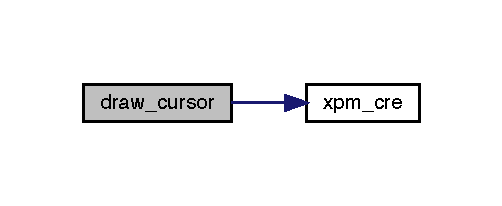
\includegraphics[width=241pt]{cursor_8c_a561698a52c09890eab87770d72706006_cgraph}
\end{center}
\end{figure}
\hypertarget{cursor_8c_ae657ac5649b0ed3caac3b9eeb26635ad}{}\label{cursor_8c_ae657ac5649b0ed3caac3b9eeb26635ad} 
\index{cursor.\+c@{cursor.\+c}!move\+\_\+cursor@{move\+\_\+cursor}}
\index{move\+\_\+cursor@{move\+\_\+cursor}!cursor.\+c@{cursor.\+c}}
\subsubsection{\texorpdfstring{move\+\_\+cursor()}{move\_cursor()}}
{\footnotesize\ttfamily void move\+\_\+cursor (\begin{DoxyParamCaption}\item[{\hyperlink{structcursor}{cursor} $\ast$}]{r1 }\end{DoxyParamCaption})}


\hypertarget{cursor_8h}{}\section{cursor.\+h File Reference}
\label{cursor_8h}\index{cursor.\+h@{cursor.\+h}}
{\ttfamily \#include \char`\"{}mouse.\+h\char`\"{}}\newline
{\ttfamily \#include \char`\"{}i8042.\+h\char`\"{}}\newline
\subsection*{Data Structures}
\begin{DoxyCompactItemize}
\item 
struct \hyperlink{structcursor}{cursor}
\end{DoxyCompactItemize}
\subsection*{Typedefs}
\begin{DoxyCompactItemize}
\item 
typedef struct \hyperlink{structcursor}{cursor} \hyperlink{cursor_8h_ac8c21e18c451143d5c49f411beb41d93}{cursor}
\end{DoxyCompactItemize}
\subsection*{Functions}
\begin{DoxyCompactItemize}
\item 
void \hyperlink{cursor_8h_a561698a52c09890eab87770d72706006}{draw\+\_\+cursor} (\hyperlink{structcursor}{cursor} r1)
\item 
void \hyperlink{cursor_8h_ae657ac5649b0ed3caac3b9eeb26635ad}{move\+\_\+cursor} (\hyperlink{structcursor}{cursor} $\ast$r1)
\end{DoxyCompactItemize}
\subsection*{Variables}
\begin{DoxyCompactItemize}
\item 
static char $\ast$ \hyperlink{cursor_8h_aa00ffb37b98a5e5e03f76299e16da73a}{cursor1} \mbox{[}$\,$\mbox{]}
\end{DoxyCompactItemize}


\subsection{Typedef Documentation}
\hypertarget{cursor_8h_ac8c21e18c451143d5c49f411beb41d93}{}\label{cursor_8h_ac8c21e18c451143d5c49f411beb41d93} 
\index{cursor.\+h@{cursor.\+h}!cursor@{cursor}}
\index{cursor@{cursor}!cursor.\+h@{cursor.\+h}}
\subsubsection{\texorpdfstring{cursor}{cursor}}
{\footnotesize\ttfamily typedef struct \hyperlink{structcursor}{cursor} \hyperlink{structcursor}{cursor}}



\subsection{Function Documentation}
\hypertarget{cursor_8h_a561698a52c09890eab87770d72706006}{}\label{cursor_8h_a561698a52c09890eab87770d72706006} 
\index{cursor.\+h@{cursor.\+h}!draw\+\_\+cursor@{draw\+\_\+cursor}}
\index{draw\+\_\+cursor@{draw\+\_\+cursor}!cursor.\+h@{cursor.\+h}}
\subsubsection{\texorpdfstring{draw\+\_\+cursor()}{draw\_cursor()}}
{\footnotesize\ttfamily void draw\+\_\+cursor (\begin{DoxyParamCaption}\item[{\hyperlink{structcursor}{cursor}}]{r1 }\end{DoxyParamCaption})}

Here is the call graph for this function\+:
\nopagebreak
\begin{figure}[H]
\begin{center}
\leavevmode
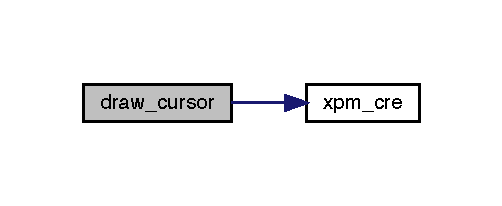
\includegraphics[width=241pt]{cursor_8h_a561698a52c09890eab87770d72706006_cgraph}
\end{center}
\end{figure}
\hypertarget{cursor_8h_ae657ac5649b0ed3caac3b9eeb26635ad}{}\label{cursor_8h_ae657ac5649b0ed3caac3b9eeb26635ad} 
\index{cursor.\+h@{cursor.\+h}!move\+\_\+cursor@{move\+\_\+cursor}}
\index{move\+\_\+cursor@{move\+\_\+cursor}!cursor.\+h@{cursor.\+h}}
\subsubsection{\texorpdfstring{move\+\_\+cursor()}{move\_cursor()}}
{\footnotesize\ttfamily void move\+\_\+cursor (\begin{DoxyParamCaption}\item[{\hyperlink{structcursor}{cursor} $\ast$}]{r1 }\end{DoxyParamCaption})}



\subsection{Variable Documentation}
\hypertarget{cursor_8h_aa00ffb37b98a5e5e03f76299e16da73a}{}\label{cursor_8h_aa00ffb37b98a5e5e03f76299e16da73a} 
\index{cursor.\+h@{cursor.\+h}!cursor1@{cursor1}}
\index{cursor1@{cursor1}!cursor.\+h@{cursor.\+h}}
\subsubsection{\texorpdfstring{cursor1}{cursor1}}
{\footnotesize\ttfamily char$\ast$ cursor1\mbox{[}$\,$\mbox{]}\hspace{0.3cm}{\ttfamily [static]}}


\hypertarget{galatic__war_8c}{}\section{galatic\+\_\+war.\+c File Reference}
\label{galatic__war_8c}\index{galatic\+\_\+war.\+c@{galatic\+\_\+war.\+c}}
{\ttfamily \#include \char`\"{}game.\+h\char`\"{}}\newline
{\ttfamily \#include \char`\"{}menu.\+h\char`\"{}}\newline
\subsection*{Functions}
\begin{DoxyCompactItemize}
\item 
int \hyperlink{galatic__war_8c_ae66f6b31b5ad750f1fe042a706a4e3d4}{main} ()
\end{DoxyCompactItemize}
\subsection*{Variables}
\begin{DoxyCompactItemize}
\item 
char \hyperlink{galatic__war_8c_aef1a4777a7043eb857234b484eb6b17b}{irq\+\_\+set}
\end{DoxyCompactItemize}


\subsection{Function Documentation}
\hypertarget{galatic__war_8c_ae66f6b31b5ad750f1fe042a706a4e3d4}{}\label{galatic__war_8c_ae66f6b31b5ad750f1fe042a706a4e3d4} 
\index{galatic\+\_\+war.\+c@{galatic\+\_\+war.\+c}!main@{main}}
\index{main@{main}!galatic\+\_\+war.\+c@{galatic\+\_\+war.\+c}}
\subsubsection{\texorpdfstring{main()}{main()}}
{\footnotesize\ttfamily int main (\begin{DoxyParamCaption}{ }\end{DoxyParamCaption})}

Here is the call graph for this function\+:
\nopagebreak
\begin{figure}[H]
\begin{center}
\leavevmode
\includegraphics[width=350pt]{galatic__war_8c_ae66f6b31b5ad750f1fe042a706a4e3d4_cgraph}
\end{center}
\end{figure}


\subsection{Variable Documentation}
\hypertarget{galatic__war_8c_aef1a4777a7043eb857234b484eb6b17b}{}\label{galatic__war_8c_aef1a4777a7043eb857234b484eb6b17b} 
\index{galatic\+\_\+war.\+c@{galatic\+\_\+war.\+c}!irq\+\_\+set@{irq\+\_\+set}}
\index{irq\+\_\+set@{irq\+\_\+set}!galatic\+\_\+war.\+c@{galatic\+\_\+war.\+c}}
\subsubsection{\texorpdfstring{irq\+\_\+set}{irq\_set}}
{\footnotesize\ttfamily char irq\+\_\+set}


\hypertarget{game_8c}{}\section{game.\+c File Reference}
\label{game_8c}\index{game.\+c@{game.\+c}}
{\ttfamily \#include \char`\"{}game.\+h\char`\"{}}\newline
\subsection*{Functions}
\begin{DoxyCompactItemize}
\item 
void \hyperlink{game_8c_ad04cb4e48ce8963b5fab5ed5fdaf29a2}{pontuation\+\_\+atual} ()
\begin{DoxyCompactList}\small\item\em draw the atual score \end{DoxyCompactList}\item 
void \hyperlink{game_8c_a4216283c98a496768ae81801c780e008}{draw} (\hyperlink{structspace__ship}{space\+\_\+ship} nv1, \hyperlink{structasteroid}{asteroid} ast1, \hyperlink{structasteroid}{asteroid} ast2)
\begin{DoxyCompactList}\small\item\em draws the objects that will be in the game \end{DoxyCompactList}\item 
int \hyperlink{game_8c_a231e4dd52378c7442957e86cb5547465}{game} ()
\begin{DoxyCompactList}\small\item\em the game \end{DoxyCompactList}\end{DoxyCompactItemize}
\subsection*{Variables}
\begin{DoxyCompactItemize}
\item 
char \hyperlink{game_8c_aef1a4777a7043eb857234b484eb6b17b}{irq\+\_\+set}
\item 
unsigned long \hyperlink{game_8c_a939081b37e8e15ed50ee75382da80da8}{global\+\_\+counter} = 0
\item 
unsigned long \hyperlink{game_8c_a3203973ba800b092636979c344e3347e}{points} = 0
\end{DoxyCompactItemize}


\subsection{Function Documentation}
\hypertarget{game_8c_a4216283c98a496768ae81801c780e008}{}\label{game_8c_a4216283c98a496768ae81801c780e008} 
\index{game.\+c@{game.\+c}!draw@{draw}}
\index{draw@{draw}!game.\+c@{game.\+c}}
\subsubsection{\texorpdfstring{draw()}{draw()}}
{\footnotesize\ttfamily void draw (\begin{DoxyParamCaption}\item[{\hyperlink{structspace__ship}{space\+\_\+ship}}]{nv1,  }\item[{\hyperlink{structasteroid}{asteroid}}]{ast1,  }\item[{\hyperlink{structasteroid}{asteroid}}]{ast2 }\end{DoxyParamCaption})}



draws the objects that will be in the game 


\begin{DoxyParams}{Parameters}
{\em nv1} & spaceship \\
\hline
{\em ast1} & one of the asteroids \\
\hline
{\em ast2} & one of the asteroids \\
\hline
\end{DoxyParams}
Here is the call graph for this function\+:
\nopagebreak
\begin{figure}[H]
\begin{center}
\leavevmode
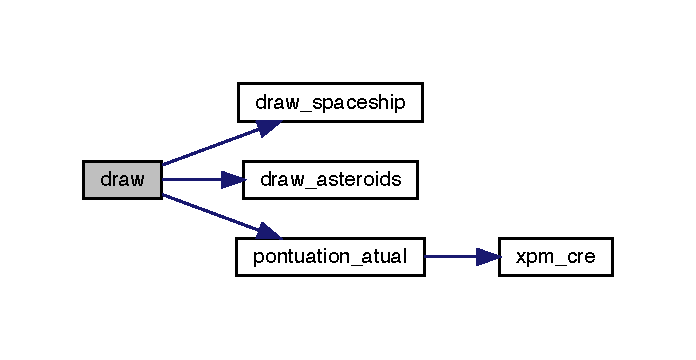
\includegraphics[width=334pt]{game_8c_a4216283c98a496768ae81801c780e008_cgraph}
\end{center}
\end{figure}
\hypertarget{game_8c_a231e4dd52378c7442957e86cb5547465}{}\label{game_8c_a231e4dd52378c7442957e86cb5547465} 
\index{game.\+c@{game.\+c}!game@{game}}
\index{game@{game}!game.\+c@{game.\+c}}
\subsubsection{\texorpdfstring{game()}{game()}}
{\footnotesize\ttfamily int game (\begin{DoxyParamCaption}{ }\end{DoxyParamCaption})}



the game 

\begin{DoxyReturn}{Returns}
0 on success or non-\/zero otherwise 
\end{DoxyReturn}
Here is the call graph for this function\+:
\nopagebreak
\begin{figure}[H]
\begin{center}
\leavevmode
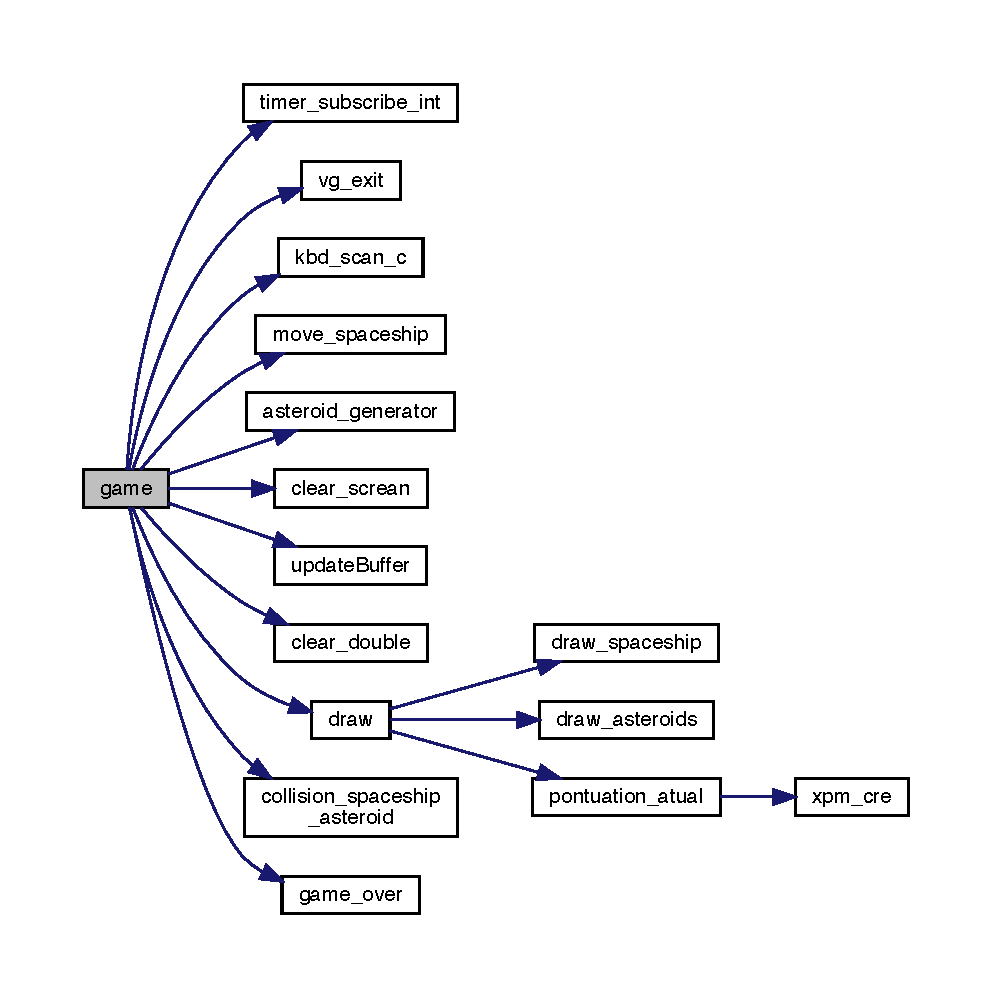
\includegraphics[width=350pt]{game_8c_a231e4dd52378c7442957e86cb5547465_cgraph}
\end{center}
\end{figure}
\hypertarget{game_8c_ad04cb4e48ce8963b5fab5ed5fdaf29a2}{}\label{game_8c_ad04cb4e48ce8963b5fab5ed5fdaf29a2} 
\index{game.\+c@{game.\+c}!pontuation\+\_\+atual@{pontuation\+\_\+atual}}
\index{pontuation\+\_\+atual@{pontuation\+\_\+atual}!game.\+c@{game.\+c}}
\subsubsection{\texorpdfstring{pontuation\+\_\+atual()}{pontuation\_atual()}}
{\footnotesize\ttfamily void pontuation\+\_\+atual (\begin{DoxyParamCaption}{ }\end{DoxyParamCaption})}



draw the atual score 

shows the player\textquotesingle{}s pontuation updated on every frame Here is the call graph for this function\+:
\nopagebreak
\begin{figure}[H]
\begin{center}
\leavevmode
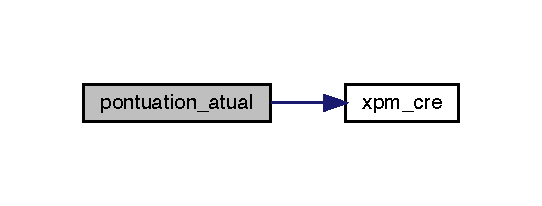
\includegraphics[width=260pt]{game_8c_ad04cb4e48ce8963b5fab5ed5fdaf29a2_cgraph}
\end{center}
\end{figure}


\subsection{Variable Documentation}
\hypertarget{game_8c_a939081b37e8e15ed50ee75382da80da8}{}\label{game_8c_a939081b37e8e15ed50ee75382da80da8} 
\index{game.\+c@{game.\+c}!global\+\_\+counter@{global\+\_\+counter}}
\index{global\+\_\+counter@{global\+\_\+counter}!game.\+c@{game.\+c}}
\subsubsection{\texorpdfstring{global\+\_\+counter}{global\_counter}}
{\footnotesize\ttfamily unsigned long global\+\_\+counter = 0}

\hypertarget{game_8c_aef1a4777a7043eb857234b484eb6b17b}{}\label{game_8c_aef1a4777a7043eb857234b484eb6b17b} 
\index{game.\+c@{game.\+c}!irq\+\_\+set@{irq\+\_\+set}}
\index{irq\+\_\+set@{irq\+\_\+set}!game.\+c@{game.\+c}}
\subsubsection{\texorpdfstring{irq\+\_\+set}{irq\_set}}
{\footnotesize\ttfamily char irq\+\_\+set}

\hypertarget{game_8c_a3203973ba800b092636979c344e3347e}{}\label{game_8c_a3203973ba800b092636979c344e3347e} 
\index{game.\+c@{game.\+c}!points@{points}}
\index{points@{points}!game.\+c@{game.\+c}}
\subsubsection{\texorpdfstring{points}{points}}
{\footnotesize\ttfamily unsigned long points = 0}


\hypertarget{game_8h}{}\section{game.\+h File Reference}
\label{game_8h}\index{game.\+h@{game.\+h}}
{\ttfamily \#include $<$minix/syslib.\+h$>$}\newline
{\ttfamily \#include $<$minix/drivers.\+h$>$}\newline
{\ttfamily \#include $<$machine/int86.\+h$>$}\newline
{\ttfamily \#include $<$minix/sysutil.\+h$>$}\newline
{\ttfamily \#include $<$minix/com.\+h$>$}\newline
{\ttfamily \#include $<$math.\+h$>$}\newline
{\ttfamily \#include $<$stdint.\+h$>$}\newline
{\ttfamily \#include \char`\"{}vbe.\+h\char`\"{}}\newline
{\ttfamily \#include \char`\"{}video\+\_\+gr.\+h\char`\"{}}\newline
{\ttfamily \#include \char`\"{}lmlib.\+h\char`\"{}}\newline
{\ttfamily \#include \char`\"{}timer.\+h\char`\"{}}\newline
{\ttfamily \#include \char`\"{}i8254.\+h\char`\"{}}\newline
{\ttfamily \#include \char`\"{}imgs.\+h\char`\"{}}\newline
{\ttfamily \#include \char`\"{}space\+\_\+ship.\+h\char`\"{}}\newline
{\ttfamily \#include \char`\"{}asteroid.\+h\char`\"{}}\newline
{\ttfamily \#include \char`\"{}collisions.\+h\char`\"{}}\newline
{\ttfamily \#include \char`\"{}game\+\_\+over.\+h\char`\"{}}\newline
{\ttfamily \#include \char`\"{}numbers.\+h\char`\"{}}\newline
\subsection*{Functions}
\begin{DoxyCompactItemize}
\item 
int \hyperlink{game_8h_a231e4dd52378c7442957e86cb5547465}{game} ()
\begin{DoxyCompactList}\small\item\em the game \end{DoxyCompactList}\item 
void \hyperlink{game_8h_a4216283c98a496768ae81801c780e008}{draw} (\hyperlink{structspace__ship}{space\+\_\+ship} nv1, \hyperlink{structasteroid}{asteroid} ast1, \hyperlink{structasteroid}{asteroid} ast2)
\begin{DoxyCompactList}\small\item\em draws the objects that will be in the game \end{DoxyCompactList}\item 
void \hyperlink{game_8h_ad04cb4e48ce8963b5fab5ed5fdaf29a2}{pontuation\+\_\+atual} ()
\begin{DoxyCompactList}\small\item\em shows the player\textquotesingle{}s pontuation updated on every frame \end{DoxyCompactList}\end{DoxyCompactItemize}


\subsection{Function Documentation}
\hypertarget{game_8h_a4216283c98a496768ae81801c780e008}{}\label{game_8h_a4216283c98a496768ae81801c780e008} 
\index{game.\+h@{game.\+h}!draw@{draw}}
\index{draw@{draw}!game.\+h@{game.\+h}}
\subsubsection{\texorpdfstring{draw()}{draw()}}
{\footnotesize\ttfamily void draw (\begin{DoxyParamCaption}\item[{\hyperlink{structspace__ship}{space\+\_\+ship}}]{nv1,  }\item[{\hyperlink{structasteroid}{asteroid}}]{ast1,  }\item[{\hyperlink{structasteroid}{asteroid}}]{ast2 }\end{DoxyParamCaption})}



draws the objects that will be in the game 


\begin{DoxyParams}{Parameters}
{\em nv1} & spaceship \\
\hline
{\em ast1} & one of the asteroids \\
\hline
{\em ast2} & one of the asteroids \\
\hline
\end{DoxyParams}
Here is the call graph for this function\+:
\nopagebreak
\begin{figure}[H]
\begin{center}
\leavevmode
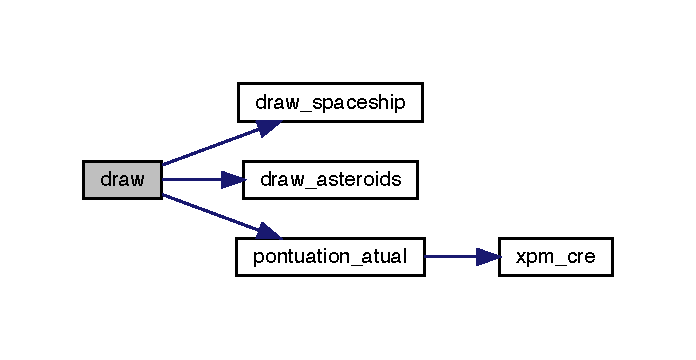
\includegraphics[width=334pt]{game_8h_a4216283c98a496768ae81801c780e008_cgraph}
\end{center}
\end{figure}
\hypertarget{game_8h_a231e4dd52378c7442957e86cb5547465}{}\label{game_8h_a231e4dd52378c7442957e86cb5547465} 
\index{game.\+h@{game.\+h}!game@{game}}
\index{game@{game}!game.\+h@{game.\+h}}
\subsubsection{\texorpdfstring{game()}{game()}}
{\footnotesize\ttfamily int game (\begin{DoxyParamCaption}{ }\end{DoxyParamCaption})}



the game 

\begin{DoxyReturn}{Returns}
0 on success or non-\/zero otherwise 
\end{DoxyReturn}
Here is the call graph for this function\+:
\nopagebreak
\begin{figure}[H]
\begin{center}
\leavevmode
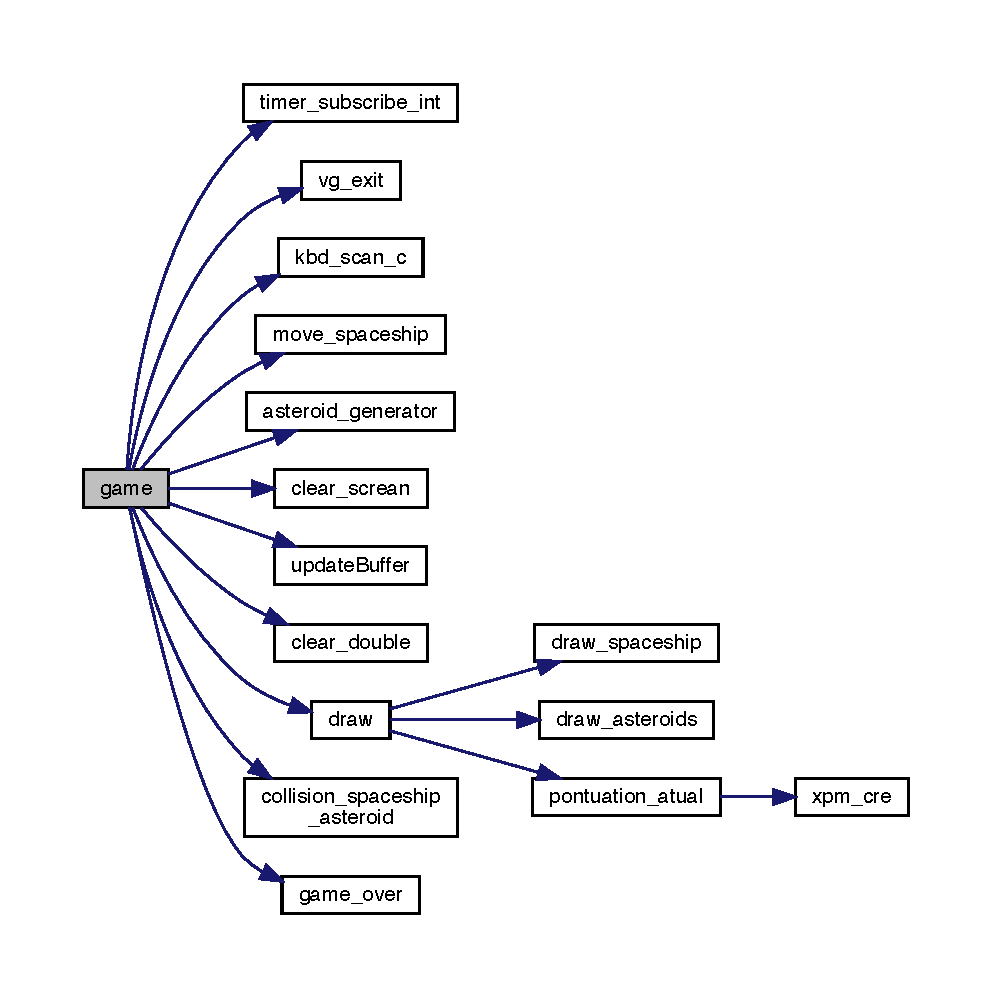
\includegraphics[width=350pt]{game_8h_a231e4dd52378c7442957e86cb5547465_cgraph}
\end{center}
\end{figure}
\hypertarget{game_8h_ad04cb4e48ce8963b5fab5ed5fdaf29a2}{}\label{game_8h_ad04cb4e48ce8963b5fab5ed5fdaf29a2} 
\index{game.\+h@{game.\+h}!pontuation\+\_\+atual@{pontuation\+\_\+atual}}
\index{pontuation\+\_\+atual@{pontuation\+\_\+atual}!game.\+h@{game.\+h}}
\subsubsection{\texorpdfstring{pontuation\+\_\+atual()}{pontuation\_atual()}}
{\footnotesize\ttfamily void pontuation\+\_\+atual (\begin{DoxyParamCaption}{ }\end{DoxyParamCaption})}



shows the player\textquotesingle{}s pontuation updated on every frame 

shows the player\textquotesingle{}s pontuation updated on every frame Here is the call graph for this function\+:
\nopagebreak
\begin{figure}[H]
\begin{center}
\leavevmode
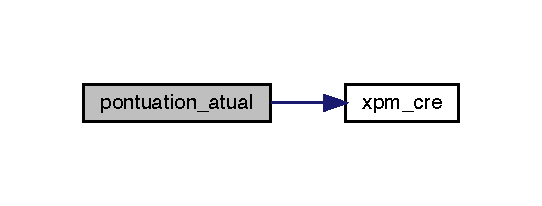
\includegraphics[width=260pt]{game_8h_ad04cb4e48ce8963b5fab5ed5fdaf29a2_cgraph}
\end{center}
\end{figure}

\hypertarget{game__over_8h}{}\section{game\+\_\+over.\+h File Reference}
\label{game__over_8h}\index{game\+\_\+over.\+h@{game\+\_\+over.\+h}}
{\ttfamily \#include \char`\"{}game.\+h\char`\"{}}\newline
{\ttfamily \#include \char`\"{}imgs\+\_\+game\+\_\+over.\+h\char`\"{}}\newline
{\ttfamily \#include \char`\"{}numbers.\+h\char`\"{}}\newline
{\ttfamily \#include \char`\"{}mouse.\+h\char`\"{}}\newline
{\ttfamily \#include \char`\"{}cursor.\+h\char`\"{}}\newline
{\ttfamily \#include \char`\"{}keyboard.\+h\char`\"{}}\newline
{\ttfamily \#include \char`\"{}math.\+h\char`\"{}}\newline
\subsection*{Data Structures}
\begin{DoxyCompactItemize}
\item 
struct \hyperlink{structimage}{image}
\end{DoxyCompactItemize}
\subsection*{Typedefs}
\begin{DoxyCompactItemize}
\item 
typedef struct \hyperlink{structimage}{image} \hyperlink{game__over_8h_a183300a528553b66677f173c07c7170e}{image}
\end{DoxyCompactItemize}
\subsection*{Functions}
\begin{DoxyCompactItemize}
\item 
int \hyperlink{game__over_8h_ae1a2e26afd9fddd52abd9795800fbfab}{game\+\_\+over} ()
\begin{DoxyCompactList}\small\item\em when a player loses the game\+\_\+over menu will appear \end{DoxyCompactList}\item 
void \hyperlink{game__over_8h_a86a18f8e6c99fff9f30c8bbc875516fc}{draw\+\_\+image} (\hyperlink{structimage}{image} t1)
\begin{DoxyCompactList}\small\item\em draws the image of the game\+\_\+over menu \end{DoxyCompactList}\item 
void \hyperlink{game__over_8h_a83353e5628621f3e651f8bcbd49efc02}{pontuation} ()
\begin{DoxyCompactList}\small\item\em shows the pontuation that the player achieve \end{DoxyCompactList}\item 
void \hyperlink{game__over_8h_a41942558c8edf2e425cbdef68805b5ee}{draw\+\_\+option} (\hyperlink{structimage}{image} ti, unsigned short option)
\begin{DoxyCompactList}\small\item\em draws the options on the Game-\/over menu \end{DoxyCompactList}\end{DoxyCompactItemize}


\subsection{Typedef Documentation}
\hypertarget{game__over_8h_a183300a528553b66677f173c07c7170e}{}\label{game__over_8h_a183300a528553b66677f173c07c7170e} 
\index{game\+\_\+over.\+h@{game\+\_\+over.\+h}!image@{image}}
\index{image@{image}!game\+\_\+over.\+h@{game\+\_\+over.\+h}}
\subsubsection{\texorpdfstring{image}{image}}
{\footnotesize\ttfamily typedef struct \hyperlink{structimage}{image} \hyperlink{structimage}{image}}



\subsection{Function Documentation}
\hypertarget{game__over_8h_a86a18f8e6c99fff9f30c8bbc875516fc}{}\label{game__over_8h_a86a18f8e6c99fff9f30c8bbc875516fc} 
\index{game\+\_\+over.\+h@{game\+\_\+over.\+h}!draw\+\_\+image@{draw\+\_\+image}}
\index{draw\+\_\+image@{draw\+\_\+image}!game\+\_\+over.\+h@{game\+\_\+over.\+h}}
\subsubsection{\texorpdfstring{draw\+\_\+image()}{draw\_image()}}
{\footnotesize\ttfamily void draw\+\_\+image (\begin{DoxyParamCaption}\item[{\hyperlink{structimage}{image}}]{t1 }\end{DoxyParamCaption})}



draws the image of the game\+\_\+over menu 


\begin{DoxyParams}{Parameters}
{\em t1} & image that will be draw \\
\hline
\end{DoxyParams}
\hypertarget{game__over_8h_a41942558c8edf2e425cbdef68805b5ee}{}\label{game__over_8h_a41942558c8edf2e425cbdef68805b5ee} 
\index{game\+\_\+over.\+h@{game\+\_\+over.\+h}!draw\+\_\+option@{draw\+\_\+option}}
\index{draw\+\_\+option@{draw\+\_\+option}!game\+\_\+over.\+h@{game\+\_\+over.\+h}}
\subsubsection{\texorpdfstring{draw\+\_\+option()}{draw\_option()}}
{\footnotesize\ttfamily void draw\+\_\+option (\begin{DoxyParamCaption}\item[{\hyperlink{structimage}{image}}]{ti,  }\item[{unsigned short}]{option }\end{DoxyParamCaption})}



draws the options on the Game-\/over menu 


\begin{DoxyParams}{Parameters}
{\em ti} & image of the option that will be draw \\
\hline
{\em option} & the number that identifies the options drawn \\
\hline
\end{DoxyParams}
\hypertarget{game__over_8h_ae1a2e26afd9fddd52abd9795800fbfab}{}\label{game__over_8h_ae1a2e26afd9fddd52abd9795800fbfab} 
\index{game\+\_\+over.\+h@{game\+\_\+over.\+h}!game\+\_\+over@{game\+\_\+over}}
\index{game\+\_\+over@{game\+\_\+over}!game\+\_\+over.\+h@{game\+\_\+over.\+h}}
\subsubsection{\texorpdfstring{game\+\_\+over()}{game\_over()}}
{\footnotesize\ttfamily int game\+\_\+over (\begin{DoxyParamCaption}{ }\end{DoxyParamCaption})}



when a player loses the game\+\_\+over menu will appear 

\begin{DoxyReturn}{Returns}
0 on success or 1 on non-\/success 
\end{DoxyReturn}
\hypertarget{game__over_8h_a83353e5628621f3e651f8bcbd49efc02}{}\label{game__over_8h_a83353e5628621f3e651f8bcbd49efc02} 
\index{game\+\_\+over.\+h@{game\+\_\+over.\+h}!pontuation@{pontuation}}
\index{pontuation@{pontuation}!game\+\_\+over.\+h@{game\+\_\+over.\+h}}
\subsubsection{\texorpdfstring{pontuation()}{pontuation()}}
{\footnotesize\ttfamily void pontuation (\begin{DoxyParamCaption}{ }\end{DoxyParamCaption})}



shows the pontuation that the player achieve 


\hypertarget{keyboard_8h}{}\section{keyboard.\+h File Reference}
\label{keyboard_8h}\index{keyboard.\+h@{keyboard.\+h}}
{\ttfamily \#include $<$minix/syslib.\+h$>$}\newline
{\ttfamily \#include $<$minix/drivers.\+h$>$}\newline
{\ttfamily \#include \char`\"{}i8042.\+h\char`\"{}}\newline
{\ttfamily \#include \char`\"{}i8254.\+h\char`\"{}}\newline
\subsection*{Functions}
\begin{DoxyCompactItemize}
\item 
int \hyperlink{keyboard_8h_a5bdf6cfb570c375192b0d87913b65c57}{kbd\+\_\+unsubscribe\+\_\+int} ()
\begin{DoxyCompactList}\small\item\em Subscribes and enables K\+BD\textquotesingle{}s interrupts. \end{DoxyCompactList}\item 
int \hyperlink{keyboard_8h_afba3a35bd6a79305e84ab4f33a5ffa7f}{kbd\+\_\+subscribe\+\_\+int} (void)
\begin{DoxyCompactList}\small\item\em Unsubscribes K\+BD\textquotesingle{}s interrupts. \end{DoxyCompactList}\item 
int \hyperlink{keyboard_8h_a5960c25178b81cfd546ba623815cfb22}{kbd\+\_\+scan\+\_\+c} (int $\ast$apt)
\begin{DoxyCompactList}\small\item\em reads the key that was pressed \end{DoxyCompactList}\item 
unsigned short \hyperlink{keyboard_8h_afc181e449b832143de81784e6e4a0bae}{read\+\_\+data\+\_\+\+O\+U\+T\+B\+U\+F\+\_\+from\+\_\+\+K\+BC} (unsigned long $\ast$data)
\begin{DoxyCompactList}\small\item\em Read K\+BC responses from Output Buffer. \end{DoxyCompactList}\item 
unsigned short \hyperlink{keyboard_8h_a5934bc1a6b9c6de87bf9f6d3b1d1f8d0}{K\+B\+C\+\_\+issue\+\_\+command\+\_\+mouse} (unsigned char command)
\begin{DoxyCompactList}\small\item\em Issues mouse command to K\+BC. \end{DoxyCompactList}\item 
unsigned short \hyperlink{keyboard_8h_a0f9b75d882918222873e81278ecfb991}{issue\+\_\+argument\+\_\+\+K\+BC} (unsigned char argument)
\begin{DoxyCompactList}\small\item\em Issues argument of any command to K\+BC. \end{DoxyCompactList}\end{DoxyCompactItemize}


\subsection{Function Documentation}
\hypertarget{keyboard_8h_a0f9b75d882918222873e81278ecfb991}{}\label{keyboard_8h_a0f9b75d882918222873e81278ecfb991} 
\index{keyboard.\+h@{keyboard.\+h}!issue\+\_\+argument\+\_\+\+K\+BC@{issue\+\_\+argument\+\_\+\+K\+BC}}
\index{issue\+\_\+argument\+\_\+\+K\+BC@{issue\+\_\+argument\+\_\+\+K\+BC}!keyboard.\+h@{keyboard.\+h}}
\subsubsection{\texorpdfstring{issue\+\_\+argument\+\_\+\+K\+B\+C()}{issue\_argument\_KBC()}}
{\footnotesize\ttfamily unsigned short issue\+\_\+argument\+\_\+\+K\+BC (\begin{DoxyParamCaption}\item[{unsigned char}]{argument }\end{DoxyParamCaption})}



Issues argument of any command to K\+BC. 


\begin{DoxyParams}{Parameters}
{\em argument} & Stores K\+BC argument from any command\\
\hline
\end{DoxyParams}
\begin{DoxyReturn}{Returns}
Return 0 upon success and non-\/zero otherwise 
\end{DoxyReturn}
\hypertarget{keyboard_8h_a5934bc1a6b9c6de87bf9f6d3b1d1f8d0}{}\label{keyboard_8h_a5934bc1a6b9c6de87bf9f6d3b1d1f8d0} 
\index{keyboard.\+h@{keyboard.\+h}!K\+B\+C\+\_\+issue\+\_\+command\+\_\+mouse@{K\+B\+C\+\_\+issue\+\_\+command\+\_\+mouse}}
\index{K\+B\+C\+\_\+issue\+\_\+command\+\_\+mouse@{K\+B\+C\+\_\+issue\+\_\+command\+\_\+mouse}!keyboard.\+h@{keyboard.\+h}}
\subsubsection{\texorpdfstring{K\+B\+C\+\_\+issue\+\_\+command\+\_\+mouse()}{KBC\_issue\_command\_mouse()}}
{\footnotesize\ttfamily unsigned short K\+B\+C\+\_\+issue\+\_\+command\+\_\+mouse (\begin{DoxyParamCaption}\item[{unsigned char}]{command }\end{DoxyParamCaption})}



Issues mouse command to K\+BC. 


\begin{DoxyParams}{Parameters}
{\em command} & Stores mouse command\\
\hline
\end{DoxyParams}
\begin{DoxyReturn}{Returns}
Return 0 upon success and non-\/zero otherwise 
\end{DoxyReturn}
\hypertarget{keyboard_8h_a5960c25178b81cfd546ba623815cfb22}{}\label{keyboard_8h_a5960c25178b81cfd546ba623815cfb22} 
\index{keyboard.\+h@{keyboard.\+h}!kbd\+\_\+scan\+\_\+c@{kbd\+\_\+scan\+\_\+c}}
\index{kbd\+\_\+scan\+\_\+c@{kbd\+\_\+scan\+\_\+c}!keyboard.\+h@{keyboard.\+h}}
\subsubsection{\texorpdfstring{kbd\+\_\+scan\+\_\+c()}{kbd\_scan\_c()}}
{\footnotesize\ttfamily int kbd\+\_\+scan\+\_\+c (\begin{DoxyParamCaption}\item[{int $\ast$}]{apt }\end{DoxyParamCaption})}



reads the key that was pressed 


\begin{DoxyParams}{Parameters}
{\em apt} & the key that was pressed\\
\hline
\end{DoxyParams}
\begin{DoxyReturn}{Returns}
0 on success or 1 on non-\/success 
\end{DoxyReturn}
\hypertarget{keyboard_8h_afba3a35bd6a79305e84ab4f33a5ffa7f}{}\label{keyboard_8h_afba3a35bd6a79305e84ab4f33a5ffa7f} 
\index{keyboard.\+h@{keyboard.\+h}!kbd\+\_\+subscribe\+\_\+int@{kbd\+\_\+subscribe\+\_\+int}}
\index{kbd\+\_\+subscribe\+\_\+int@{kbd\+\_\+subscribe\+\_\+int}!keyboard.\+h@{keyboard.\+h}}
\subsubsection{\texorpdfstring{kbd\+\_\+subscribe\+\_\+int()}{kbd\_subscribe\_int()}}
{\footnotesize\ttfamily int kbd\+\_\+subscribe\+\_\+int (\begin{DoxyParamCaption}\item[{void}]{ }\end{DoxyParamCaption})}



Unsubscribes K\+BD\textquotesingle{}s interrupts. 

\begin{DoxyReturn}{Returns}
Return 0 upon success and non-\/zero otherwise 
\end{DoxyReturn}
\hypertarget{keyboard_8h_a5bdf6cfb570c375192b0d87913b65c57}{}\label{keyboard_8h_a5bdf6cfb570c375192b0d87913b65c57} 
\index{keyboard.\+h@{keyboard.\+h}!kbd\+\_\+unsubscribe\+\_\+int@{kbd\+\_\+unsubscribe\+\_\+int}}
\index{kbd\+\_\+unsubscribe\+\_\+int@{kbd\+\_\+unsubscribe\+\_\+int}!keyboard.\+h@{keyboard.\+h}}
\subsubsection{\texorpdfstring{kbd\+\_\+unsubscribe\+\_\+int()}{kbd\_unsubscribe\_int()}}
{\footnotesize\ttfamily int kbd\+\_\+unsubscribe\+\_\+int (\begin{DoxyParamCaption}{ }\end{DoxyParamCaption})}



Subscribes and enables K\+BD\textquotesingle{}s interrupts. 

\begin{DoxyReturn}{Returns}
Returns bit order in interrupt mask; negative value on failure 
\end{DoxyReturn}
\hypertarget{keyboard_8h_afc181e449b832143de81784e6e4a0bae}{}\label{keyboard_8h_afc181e449b832143de81784e6e4a0bae} 
\index{keyboard.\+h@{keyboard.\+h}!read\+\_\+data\+\_\+\+O\+U\+T\+B\+U\+F\+\_\+from\+\_\+\+K\+BC@{read\+\_\+data\+\_\+\+O\+U\+T\+B\+U\+F\+\_\+from\+\_\+\+K\+BC}}
\index{read\+\_\+data\+\_\+\+O\+U\+T\+B\+U\+F\+\_\+from\+\_\+\+K\+BC@{read\+\_\+data\+\_\+\+O\+U\+T\+B\+U\+F\+\_\+from\+\_\+\+K\+BC}!keyboard.\+h@{keyboard.\+h}}
\subsubsection{\texorpdfstring{read\+\_\+data\+\_\+\+O\+U\+T\+B\+U\+F\+\_\+from\+\_\+\+K\+B\+C()}{read\_data\_OUTBUF\_from\_KBC()}}
{\footnotesize\ttfamily unsigned short read\+\_\+data\+\_\+\+O\+U\+T\+B\+U\+F\+\_\+from\+\_\+\+K\+BC (\begin{DoxyParamCaption}\item[{unsigned long $\ast$}]{data }\end{DoxyParamCaption})}



Read K\+BC responses from Output Buffer. 


\begin{DoxyParams}{Parameters}
{\em data} & Stores K\+BC Response (A\+CK, R\+E\+S\+E\+ND, E\+R\+R\+OR)\\
\hline
\end{DoxyParams}
\begin{DoxyReturn}{Returns}
Return 0 upon success or non-\/zero otherwise 
\end{DoxyReturn}

\hypertarget{lmlib_8h}{}\section{lmlib.\+h File Reference}
\label{lmlib_8h}\index{lmlib.\+h@{lmlib.\+h}}
\subsection*{Data Structures}
\begin{DoxyCompactItemize}
\item 
struct \hyperlink{structmmap__t}{mmap\+\_\+t}
\end{DoxyCompactItemize}
\subsection*{Functions}
\begin{DoxyCompactItemize}
\item 
void $\ast$ \hyperlink{group__lmlib_ga00a9c17c01e794a6bfc80fc5c6ab1ed1}{lm\+\_\+init} (void)
\begin{DoxyCompactList}\small\item\em Initializes the low memory area, the region up to the 1 M\+Byte physical address, by mapping it on the process\textquotesingle{} physical memory address. \end{DoxyCompactList}\item 
void $\ast$ \hyperlink{group__lmlib_gae45d971ce2ffcf4dc2677eba033a92cd}{lm\+\_\+alloc} (unsigned long size, \hyperlink{structmmap__t}{mmap\+\_\+t} $\ast$map)
\begin{DoxyCompactList}\small\item\em Allocates a memory block in low memory area with the specified size. \end{DoxyCompactList}\item 
void \hyperlink{group__lmlib_ga73e89d9c297b7390021fb545513579c6}{lm\+\_\+free} (\hyperlink{structmmap__t}{mmap\+\_\+t} $\ast$map)
\begin{DoxyCompactList}\small\item\em Frees a memory block in the low memory area, previously allocated using \hyperlink{group__lmlib_gae45d971ce2ffcf4dc2677eba033a92cd}{lm\+\_\+alloc()} \end{DoxyCompactList}\end{DoxyCompactItemize}

\hypertarget{menu_8h}{}\section{menu.\+h File Reference}
\label{menu_8h}\index{menu.\+h@{menu.\+h}}
{\ttfamily \#include \char`\"{}game.\+h\char`\"{}}\newline
{\ttfamily \#include \char`\"{}imgs\+\_\+menu.\+h\char`\"{}}\newline
{\ttfamily \#include \char`\"{}mouse.\+h\char`\"{}}\newline
{\ttfamily \#include \char`\"{}cursor.\+h\char`\"{}}\newline
{\ttfamily \#include \char`\"{}game\+\_\+over.\+h\char`\"{}}\newline
{\ttfamily \#include \char`\"{}R\+T\+C.\+h\char`\"{}}\newline
\subsection*{Data Structures}
\begin{DoxyCompactItemize}
\item 
struct \hyperlink{structimg}{img}
\end{DoxyCompactItemize}
\subsection*{Typedefs}
\begin{DoxyCompactItemize}
\item 
typedef struct \hyperlink{structimg}{img} \hyperlink{menu_8h_a9d0cf302c442de0fa71b8e3a56f70c24}{img}
\end{DoxyCompactItemize}
\subsection*{Functions}
\begin{DoxyCompactItemize}
\item 
void \hyperlink{menu_8h_ab74b5533cfd5daca9ed03628346c26d6}{data\+\_\+sistema} ()
\begin{DoxyCompactList}\small\item\em shows the date \end{DoxyCompactList}\item 
int \hyperlink{menu_8h_ae83fcdbeb2b6757fc741ae953b633ee1}{menu} ()
\begin{DoxyCompactList}\small\item\em the main menu \end{DoxyCompactList}\item 
void \hyperlink{menu_8h_a060d18aba3cc764133196b57f3bb7de9}{draw\+\_\+img} (\hyperlink{structimg}{img} ti)
\begin{DoxyCompactList}\small\item\em draw the backgroud of the menu \end{DoxyCompactList}\end{DoxyCompactItemize}


\subsection{Typedef Documentation}
\hypertarget{menu_8h_a9d0cf302c442de0fa71b8e3a56f70c24}{}\label{menu_8h_a9d0cf302c442de0fa71b8e3a56f70c24} 
\index{menu.\+h@{menu.\+h}!img@{img}}
\index{img@{img}!menu.\+h@{menu.\+h}}
\subsubsection{\texorpdfstring{img}{img}}
{\footnotesize\ttfamily typedef struct \hyperlink{structimg}{img} \hyperlink{structimg}{img}}



\subsection{Function Documentation}
\hypertarget{menu_8h_ab74b5533cfd5daca9ed03628346c26d6}{}\label{menu_8h_ab74b5533cfd5daca9ed03628346c26d6} 
\index{menu.\+h@{menu.\+h}!data\+\_\+sistema@{data\+\_\+sistema}}
\index{data\+\_\+sistema@{data\+\_\+sistema}!menu.\+h@{menu.\+h}}
\subsubsection{\texorpdfstring{data\+\_\+sistema()}{data\_sistema()}}
{\footnotesize\ttfamily void data\+\_\+sistema (\begin{DoxyParamCaption}{ }\end{DoxyParamCaption})}



shows the date 

\hypertarget{menu_8h_a060d18aba3cc764133196b57f3bb7de9}{}\label{menu_8h_a060d18aba3cc764133196b57f3bb7de9} 
\index{menu.\+h@{menu.\+h}!draw\+\_\+img@{draw\+\_\+img}}
\index{draw\+\_\+img@{draw\+\_\+img}!menu.\+h@{menu.\+h}}
\subsubsection{\texorpdfstring{draw\+\_\+img()}{draw\_img()}}
{\footnotesize\ttfamily void draw\+\_\+img (\begin{DoxyParamCaption}\item[{\hyperlink{structimg}{img}}]{ti }\end{DoxyParamCaption})}



draw the backgroud of the menu 


\begin{DoxyParams}{Parameters}
{\em ti} & the background image \\
\hline
\end{DoxyParams}
\hypertarget{menu_8h_ae83fcdbeb2b6757fc741ae953b633ee1}{}\label{menu_8h_ae83fcdbeb2b6757fc741ae953b633ee1} 
\index{menu.\+h@{menu.\+h}!menu@{menu}}
\index{menu@{menu}!menu.\+h@{menu.\+h}}
\subsubsection{\texorpdfstring{menu()}{menu()}}
{\footnotesize\ttfamily int menu (\begin{DoxyParamCaption}{ }\end{DoxyParamCaption})}



the main menu 

\begin{DoxyReturn}{Returns}
0 on success or non-\/zero otherwise 
\end{DoxyReturn}

\hypertarget{mouse_8c}{}\section{mouse.\+c File Reference}
\label{mouse_8c}\index{mouse.\+c@{mouse.\+c}}
{\ttfamily \#include \char`\"{}mouse.\+h\char`\"{}}\newline
{\ttfamily \#include \char`\"{}i8042.\+h\char`\"{}}\newline
{\ttfamily \#include \char`\"{}keyboard.\+h\char`\"{}}\newline
\subsection*{Functions}
\begin{DoxyCompactItemize}
\item 
int \hyperlink{mouse_8c_a99506573209b197b84ee22a228b89fbd}{mouse\+\_\+subscribe\+\_\+int} ()
\begin{DoxyCompactList}\small\item\em Subscribes and enables Mouse interrupts. \end{DoxyCompactList}\item 
int \hyperlink{mouse_8c_abb62339e13d96f9050f69a71428f8eb9}{mouse\+\_\+unsubscribe} ()
\begin{DoxyCompactList}\small\item\em Unsubscribes Mouse interrupts. \end{DoxyCompactList}\end{DoxyCompactItemize}


\subsection{Function Documentation}
\hypertarget{mouse_8c_a99506573209b197b84ee22a228b89fbd}{}\label{mouse_8c_a99506573209b197b84ee22a228b89fbd} 
\index{mouse.\+c@{mouse.\+c}!mouse\+\_\+subscribe\+\_\+int@{mouse\+\_\+subscribe\+\_\+int}}
\index{mouse\+\_\+subscribe\+\_\+int@{mouse\+\_\+subscribe\+\_\+int}!mouse.\+c@{mouse.\+c}}
\subsubsection{\texorpdfstring{mouse\+\_\+subscribe\+\_\+int()}{mouse\_subscribe\_int()}}
{\footnotesize\ttfamily int mouse\+\_\+subscribe\+\_\+int (\begin{DoxyParamCaption}{ }\end{DoxyParamCaption})}



Subscribes and enables Mouse interrupts. 

\begin{DoxyReturn}{Returns}
Returns bit order in interrupt mask; negative value on failure 
\end{DoxyReturn}
\hypertarget{mouse_8c_abb62339e13d96f9050f69a71428f8eb9}{}\label{mouse_8c_abb62339e13d96f9050f69a71428f8eb9} 
\index{mouse.\+c@{mouse.\+c}!mouse\+\_\+unsubscribe@{mouse\+\_\+unsubscribe}}
\index{mouse\+\_\+unsubscribe@{mouse\+\_\+unsubscribe}!mouse.\+c@{mouse.\+c}}
\subsubsection{\texorpdfstring{mouse\+\_\+unsubscribe()}{mouse\_unsubscribe()}}
{\footnotesize\ttfamily int mouse\+\_\+unsubscribe (\begin{DoxyParamCaption}{ }\end{DoxyParamCaption})}



Unsubscribes Mouse interrupts. 

\begin{DoxyReturn}{Returns}
Return 0 upon success and non-\/zero otherwise 
\end{DoxyReturn}

\hypertarget{mouse_8h}{}\section{mouse.\+h File Reference}
\label{mouse_8h}\index{mouse.\+h@{mouse.\+h}}
{\ttfamily \#include $<$minix/syslib.\+h$>$}\newline
{\ttfamily \#include $<$minix/drivers.\+h$>$}\newline
{\ttfamily \#include $<$minix/com.\+h$>$}\newline
{\ttfamily \#include $<$stdio.\+h$>$}\newline
{\ttfamily \#include $<$stdlib.\+h$>$}\newline
{\ttfamily \#include $<$minix/sysutil.\+h$>$}\newline
\subsection*{Functions}
\begin{DoxyCompactItemize}
\item 
int \hyperlink{mouse_8h_a99506573209b197b84ee22a228b89fbd}{mouse\+\_\+subscribe\+\_\+int} ()
\begin{DoxyCompactList}\small\item\em Subscribes and enables Mouse interrupts. \end{DoxyCompactList}\item 
int \hyperlink{mouse_8h_abb62339e13d96f9050f69a71428f8eb9}{mouse\+\_\+unsubscribe} ()
\begin{DoxyCompactList}\small\item\em Unsubscribes Mouse interrupts. \end{DoxyCompactList}\end{DoxyCompactItemize}
\subsection*{Variables}
\begin{DoxyCompactItemize}
\item 
static int \hyperlink{mouse_8h_a0b0da21bbdff62b7b28e9af7ec3d0d76}{hook\+\_\+id\+\_\+mouse} = 12
\item 
unsigned long \hyperlink{mouse_8h_adbf067b12d66e0b4c1afe05331fe4edb}{packet} \mbox{[}3\mbox{]}
\item 
static int \hyperlink{mouse_8h_a2e61911f80e72e76b6906f5044d86b76}{byte\+\_\+number} = 0
\end{DoxyCompactItemize}


\subsection{Function Documentation}
\hypertarget{mouse_8h_a99506573209b197b84ee22a228b89fbd}{}\label{mouse_8h_a99506573209b197b84ee22a228b89fbd} 
\index{mouse.\+h@{mouse.\+h}!mouse\+\_\+subscribe\+\_\+int@{mouse\+\_\+subscribe\+\_\+int}}
\index{mouse\+\_\+subscribe\+\_\+int@{mouse\+\_\+subscribe\+\_\+int}!mouse.\+h@{mouse.\+h}}
\subsubsection{\texorpdfstring{mouse\+\_\+subscribe\+\_\+int()}{mouse\_subscribe\_int()}}
{\footnotesize\ttfamily int mouse\+\_\+subscribe\+\_\+int (\begin{DoxyParamCaption}{ }\end{DoxyParamCaption})}



Subscribes and enables Mouse interrupts. 

\begin{DoxyReturn}{Returns}
Returns bit order in interrupt mask; negative value on failure 
\end{DoxyReturn}
\hypertarget{mouse_8h_abb62339e13d96f9050f69a71428f8eb9}{}\label{mouse_8h_abb62339e13d96f9050f69a71428f8eb9} 
\index{mouse.\+h@{mouse.\+h}!mouse\+\_\+unsubscribe@{mouse\+\_\+unsubscribe}}
\index{mouse\+\_\+unsubscribe@{mouse\+\_\+unsubscribe}!mouse.\+h@{mouse.\+h}}
\subsubsection{\texorpdfstring{mouse\+\_\+unsubscribe()}{mouse\_unsubscribe()}}
{\footnotesize\ttfamily int mouse\+\_\+unsubscribe (\begin{DoxyParamCaption}{ }\end{DoxyParamCaption})}



Unsubscribes Mouse interrupts. 

\begin{DoxyReturn}{Returns}
Return 0 upon success and non-\/zero otherwise 
\end{DoxyReturn}


\subsection{Variable Documentation}
\hypertarget{mouse_8h_a2e61911f80e72e76b6906f5044d86b76}{}\label{mouse_8h_a2e61911f80e72e76b6906f5044d86b76} 
\index{mouse.\+h@{mouse.\+h}!byte\+\_\+number@{byte\+\_\+number}}
\index{byte\+\_\+number@{byte\+\_\+number}!mouse.\+h@{mouse.\+h}}
\subsubsection{\texorpdfstring{byte\+\_\+number}{byte\_number}}
{\footnotesize\ttfamily int byte\+\_\+number = 0\hspace{0.3cm}{\ttfamily [static]}}

\hypertarget{mouse_8h_a0b0da21bbdff62b7b28e9af7ec3d0d76}{}\label{mouse_8h_a0b0da21bbdff62b7b28e9af7ec3d0d76} 
\index{mouse.\+h@{mouse.\+h}!hook\+\_\+id\+\_\+mouse@{hook\+\_\+id\+\_\+mouse}}
\index{hook\+\_\+id\+\_\+mouse@{hook\+\_\+id\+\_\+mouse}!mouse.\+h@{mouse.\+h}}
\subsubsection{\texorpdfstring{hook\+\_\+id\+\_\+mouse}{hook\_id\_mouse}}
{\footnotesize\ttfamily int hook\+\_\+id\+\_\+mouse = 12\hspace{0.3cm}{\ttfamily [static]}}

\hypertarget{mouse_8h_adbf067b12d66e0b4c1afe05331fe4edb}{}\label{mouse_8h_adbf067b12d66e0b4c1afe05331fe4edb} 
\index{mouse.\+h@{mouse.\+h}!packet@{packet}}
\index{packet@{packet}!mouse.\+h@{mouse.\+h}}
\subsubsection{\texorpdfstring{packet}{packet}}
{\footnotesize\ttfamily unsigned long packet\mbox{[}3\mbox{]}}


\hypertarget{space__ship_8h}{}\section{space\+\_\+ship.\+h File Reference}
\label{space__ship_8h}\index{space\+\_\+ship.\+h@{space\+\_\+ship.\+h}}
\subsection*{Data Structures}
\begin{DoxyCompactItemize}
\item 
struct \hyperlink{structspace__ship}{space\+\_\+ship}
\end{DoxyCompactItemize}
\subsection*{Typedefs}
\begin{DoxyCompactItemize}
\item 
typedef struct \hyperlink{structspace__ship}{space\+\_\+ship} \hyperlink{space__ship_8h_ae45b381859410b8de3363b4e200b47ea}{space\+\_\+ship}
\end{DoxyCompactItemize}
\subsection*{Functions}
\begin{DoxyCompactItemize}
\item 
int \hyperlink{space__ship_8h_ad01afb3a3ddb0ad991fb22d23bf0b0a6}{move\+\_\+spaceship} (\hyperlink{structspace__ship}{space\+\_\+ship} $\ast$nv1, short delta)
\begin{DoxyCompactList}\small\item\em moves the spaceship \end{DoxyCompactList}\item 
void \hyperlink{space__ship_8h_ae4d0cb9056d3e9ea3918ba7d9a6894fc}{draw\+\_\+spaceship} (\hyperlink{structspace__ship}{space\+\_\+ship} nv1)
\begin{DoxyCompactList}\small\item\em draws a spaceship \end{DoxyCompactList}\end{DoxyCompactItemize}


\subsection{Typedef Documentation}
\hypertarget{space__ship_8h_ae45b381859410b8de3363b4e200b47ea}{}\label{space__ship_8h_ae45b381859410b8de3363b4e200b47ea} 
\index{space\+\_\+ship.\+h@{space\+\_\+ship.\+h}!space\+\_\+ship@{space\+\_\+ship}}
\index{space\+\_\+ship@{space\+\_\+ship}!space\+\_\+ship.\+h@{space\+\_\+ship.\+h}}
\subsubsection{\texorpdfstring{space\+\_\+ship}{space\_ship}}
{\footnotesize\ttfamily typedef struct \hyperlink{structspace__ship}{space\+\_\+ship} \hyperlink{structspace__ship}{space\+\_\+ship}}



\subsection{Function Documentation}
\hypertarget{space__ship_8h_ae4d0cb9056d3e9ea3918ba7d9a6894fc}{}\label{space__ship_8h_ae4d0cb9056d3e9ea3918ba7d9a6894fc} 
\index{space\+\_\+ship.\+h@{space\+\_\+ship.\+h}!draw\+\_\+spaceship@{draw\+\_\+spaceship}}
\index{draw\+\_\+spaceship@{draw\+\_\+spaceship}!space\+\_\+ship.\+h@{space\+\_\+ship.\+h}}
\subsubsection{\texorpdfstring{draw\+\_\+spaceship()}{draw\_spaceship()}}
{\footnotesize\ttfamily void draw\+\_\+spaceship (\begin{DoxyParamCaption}\item[{\hyperlink{structspace__ship}{space\+\_\+ship}}]{nv1 }\end{DoxyParamCaption})}



draws a spaceship 


\begin{DoxyParams}{Parameters}
{\em nv1} & the spaceship that will be draw \\
\hline
\end{DoxyParams}
\hypertarget{space__ship_8h_ad01afb3a3ddb0ad991fb22d23bf0b0a6}{}\label{space__ship_8h_ad01afb3a3ddb0ad991fb22d23bf0b0a6} 
\index{space\+\_\+ship.\+h@{space\+\_\+ship.\+h}!move\+\_\+spaceship@{move\+\_\+spaceship}}
\index{move\+\_\+spaceship@{move\+\_\+spaceship}!space\+\_\+ship.\+h@{space\+\_\+ship.\+h}}
\subsubsection{\texorpdfstring{move\+\_\+spaceship()}{move\_spaceship()}}
{\footnotesize\ttfamily int move\+\_\+spaceship (\begin{DoxyParamCaption}\item[{\hyperlink{structspace__ship}{space\+\_\+ship} $\ast$}]{nv1,  }\item[{short}]{delta }\end{DoxyParamCaption})}



moves the spaceship 


\begin{DoxyParams}{Parameters}
{\em nv1} & the spaceship that will be moved \\
\hline
{\em delta} & the number of pixels that the spaceship will be moved \\
\hline
\end{DoxyParams}
\begin{DoxyReturn}{Returns}
0 on success or non-\/zero otherwise 
\end{DoxyReturn}

\hypertarget{timer_8h}{}\section{timer.\+h File Reference}
\label{timer_8h}\index{timer.\+h@{timer.\+h}}
{\ttfamily \#include $<$minix/syslib.\+h$>$}\newline
{\ttfamily \#include $<$minix/drivers.\+h$>$}\newline
{\ttfamily \#include \char`\"{}i8254.\+h\char`\"{}}\newline
\subsection*{Functions}
\begin{DoxyCompactItemize}
\item 
int \hyperlink{timer_8h_a4c5d9f47323eda494cfd826f6d62eec9}{timer\+\_\+subscribe\+\_\+int} (void)
\begin{DoxyCompactList}\small\item\em Subscribes and enables Timer 0 interrupts. \end{DoxyCompactList}\item 
int \hyperlink{timer_8h_ab9eea51549744bca5c5c923b388bb4ee}{timer\+\_\+unsubscribe\+\_\+int} ()
\begin{DoxyCompactList}\small\item\em Unsubscribes Timer 0 interrupts. \end{DoxyCompactList}\end{DoxyCompactItemize}


\subsection{Function Documentation}
\hypertarget{timer_8h_a4c5d9f47323eda494cfd826f6d62eec9}{}\label{timer_8h_a4c5d9f47323eda494cfd826f6d62eec9} 
\index{timer.\+h@{timer.\+h}!timer\+\_\+subscribe\+\_\+int@{timer\+\_\+subscribe\+\_\+int}}
\index{timer\+\_\+subscribe\+\_\+int@{timer\+\_\+subscribe\+\_\+int}!timer.\+h@{timer.\+h}}
\subsubsection{\texorpdfstring{timer\+\_\+subscribe\+\_\+int()}{timer\_subscribe\_int()}}
{\footnotesize\ttfamily int timer\+\_\+subscribe\+\_\+int (\begin{DoxyParamCaption}\item[{void}]{ }\end{DoxyParamCaption})}



Subscribes and enables Timer 0 interrupts. 

\begin{DoxyReturn}{Returns}
Returns bit order in interrupt mask; negative value on failure 
\end{DoxyReturn}
\hypertarget{timer_8h_ab9eea51549744bca5c5c923b388bb4ee}{}\label{timer_8h_ab9eea51549744bca5c5c923b388bb4ee} 
\index{timer.\+h@{timer.\+h}!timer\+\_\+unsubscribe\+\_\+int@{timer\+\_\+unsubscribe\+\_\+int}}
\index{timer\+\_\+unsubscribe\+\_\+int@{timer\+\_\+unsubscribe\+\_\+int}!timer.\+h@{timer.\+h}}
\subsubsection{\texorpdfstring{timer\+\_\+unsubscribe\+\_\+int()}{timer\_unsubscribe\_int()}}
{\footnotesize\ttfamily int timer\+\_\+unsubscribe\+\_\+int (\begin{DoxyParamCaption}{ }\end{DoxyParamCaption})}



Unsubscribes Timer 0 interrupts. 

\begin{DoxyReturn}{Returns}
Return 0 upon success and non-\/zero otherwise 
\end{DoxyReturn}

\hypertarget{vbe_8h}{}\section{vbe.\+h File Reference}
\label{vbe_8h}\index{vbe.\+h@{vbe.\+h}}
{\ttfamily \#include $<$stdint.\+h$>$}\newline
\subsection*{Data Structures}
\begin{DoxyCompactItemize}
\item 
struct \hyperlink{struct____attribute____}{\+\_\+\+\_\+attribute\+\_\+\+\_\+}
\end{DoxyCompactItemize}
\subsection*{Macros}
\begin{DoxyCompactItemize}
\item 
\#define \hyperlink{vbe_8h_ab208dc4bc0e43eff7f62a8841dcf6cb5}{V\+B\+E\+\_\+\+M\+O\+DE}~0x4\+F02
\item 
\#define \hyperlink{vbe_8h_aba209728590d097395cf004cb397e160}{V\+B\+E\+\_\+\+G\+E\+T\+\_\+\+M\+O\+DE}~0x4\+F01
\item 
\#define \hyperlink{vbe_8h_a58367b07d97797b17b41dd76e3d087c3}{V\+B\+E\+\_\+\+C\+O\+N\+T\+R\+O\+L\+\_\+\+I\+N\+FO}~0x4\+F00
\item 
\#define \hyperlink{vbe_8h_a717c0759fff3411820f5b372b8d07db4}{I\+N\+T\+E\+R\+R\+U\+P\+T\+\_\+\+V\+BE}~0x10
\item 
\#define \hyperlink{vbe_8h_a0aae61f24e1156f489dfda729685fa9c}{G\+R\+A\+P\+H\+I\+C\+\_\+\+M\+O\+DE}~0x105
\item 
\#define \hyperlink{vbe_8h_a6b5d73667b04f2f103f3ee6bea21cf23}{V\+B\+E\+\_\+\+M\+O\+D\+E\+\_\+\+S\+I\+ZE}~256
\item 
\#define \hyperlink{vbe_8h_a3a8ea58898cb58fc96013383d39f482c}{B\+IT}(n)~(0x01$<$$<$(n))
\item 
\#define \hyperlink{vbe_8h_a30bf84c312af248cb81bb224e09f9ba8}{T\+I\+M\+E\+R0\+\_\+\+I\+RQ}~0
\item 
\#define \hyperlink{vbe_8h_a1a522aa19bcb695a9df30032a893bee3}{D\+E\+L\+A\+Y\+\_\+\+US}~20000
\item 
\#define \hyperlink{vbe_8h_a89c4d098b53809674457b1660b1af780}{S\+T\+A\+T\+\_\+\+R\+EG}~0\+X64
\item 
\#define \hyperlink{vbe_8h_a6d57c7927a10f638c83046b52c8caac9}{K\+B\+C\+\_\+\+C\+M\+D\+\_\+\+R\+EG}~0x64
\item 
\#define \hyperlink{vbe_8h_acfb42dde389e8ca36ab267002fbf5c6a}{O\+U\+T\+\_\+\+B\+UF}~0x60
\item 
\#define \hyperlink{vbe_8h_a307ab71673e26ec42b28a3bca05d4cb5}{P\+A\+R\+\_\+\+E\+RR}~0x80
\item 
\#define \hyperlink{vbe_8h_ad16f61e2bf70f6c7685e826224ed177f}{T\+O\+\_\+\+E\+RR}~0x40
\item 
\#define \hyperlink{vbe_8h_ac16d7b9842f2c912281317f31786c31f}{C\+B\+U\+F\+F\+E\+R\+\_\+\+E\+K\+BD}~0x\+F4
\item 
\#define \hyperlink{vbe_8h_a61686d33603491344883775b9b31e172}{L\+E\+DS}~0x\+ED
\item 
\#define \hyperlink{vbe_8h_a6f6489887e08bff4887d0bc5dcf214d8}{A\+CK}~0x00\+FA
\item 
\#define \hyperlink{vbe_8h_a92f67631ef5a97e4a266c15bc710776d}{R\+E\+S\+E\+ND}~0x\+FE
\item 
\#define \hyperlink{vbe_8h_a8fe83ac76edc595f6b98cd4a4127aed5}{E\+R\+R\+OR}~0x\+FC
\item 
\#define \hyperlink{vbe_8h_aa6addd819c1594c0f9285169048db5ab}{K\+B\+D\+\_\+\+E\+S\+C\+\_\+\+K\+EY}~0x81
\item 
\#define \hyperlink{vbe_8h_a1cc261de4fdcbf43464428947a52ce32}{R\+I\+G\+H\+T\+\_\+\+K\+EY}~0x\+CD
\item 
\#define \hyperlink{vbe_8h_a3cd87a710fd069baf487e7b44d01e1b9}{L\+E\+F\+T\+\_\+\+K\+EY}~0x\+CB
\item 
\#define \hyperlink{vbe_8h_a1c34fc6f48366ae6334736730fd9b0e7}{U\+P\+\_\+\+K\+EY}~0x\+C8
\item 
\#define \hyperlink{vbe_8h_a687b69f632086f6e1a03279964257c24}{D\+O\+W\+N\+\_\+\+K\+EY}~0x\+D0
\item 
\#define \hyperlink{vbe_8h_af4bced5cf8ed55746d4b5d34f9a0fe39}{E\+N\+T\+ER}~0x9C
\end{DoxyCompactItemize}
\subsection*{Functions}
\begin{Indent}{\bf V\+BE Mode Info Block}\par
\begin{DoxyCompactItemize}
\item 
int \hyperlink{group__vbe_ga6434e88ed32e7458f821d28c25a3ef48}{vbe\+\_\+set\+\_\+mode} (unsigned short function, unsigned short mode)
\begin{DoxyCompactList}\small\item\em sets the V\+BE mode \end{DoxyCompactList}\item 
int \hyperlink{group__vbe_ga4ef3234e41f2050bc094a22049b69e45}{vbe\+\_\+get\+\_\+mode\+\_\+info} (unsigned short mode, vbe\+\_\+mode\+\_\+info\+\_\+t $\ast$vmi\+\_\+p)
\begin{DoxyCompactList}\small\item\em Returns information on the input V\+BE mode, including screen dimensions, color depth and V\+R\+AM physical address. \end{DoxyCompactList}\item 
char $\ast$ \hyperlink{group__vbe_ga87bd140b1b1b28386f37ebac5c9b9d2e}{read\+\_\+xpm} (char $\ast$map\mbox{[}$\,$\mbox{]}, int $\ast$width, int $\ast$height)
\begin{DoxyCompactList}\small\item\em reads a xpm with a width and a height \end{DoxyCompactList}\item 
int \hyperlink{group__vbe_ga4977ce5be211025d9fd499e2f849f684}{xpm\+\_\+cre} (int $\ast$altura, int $\ast$largura, unsigned short x, unsigned short y, char $\ast$xpm\mbox{[}$\,$\mbox{]})
\item 
int \hyperlink{group__vbe_ga045215cbe9b4eaf41f594066d77dcaf4}{xpm\+\_\+del} (int $\ast$altura, int $\ast$largura, unsigned short x, unsigned short y)
\begin{DoxyCompactList}\small\item\em deletes a xpm \end{DoxyCompactList}\end{DoxyCompactItemize}
\end{Indent}
\subsection*{Variables}
\begin{DoxyCompactItemize}
\item 
int \hyperlink{vbe_8h_a96f78a87d064e47d627d222f67a8d012}{hook\+\_\+id}
\item 
int \hyperlink{vbe_8h_a5505b5dc8d9e5d894a7ac2626a106e13}{khook\+\_\+id}
\end{DoxyCompactItemize}


\subsection{Macro Definition Documentation}
\hypertarget{vbe_8h_a6f6489887e08bff4887d0bc5dcf214d8}{}\label{vbe_8h_a6f6489887e08bff4887d0bc5dcf214d8} 
\index{vbe.\+h@{vbe.\+h}!A\+CK@{A\+CK}}
\index{A\+CK@{A\+CK}!vbe.\+h@{vbe.\+h}}
\subsubsection{\texorpdfstring{A\+CK}{ACK}}
{\footnotesize\ttfamily \#define A\+CK~0x00\+FA}

\hypertarget{vbe_8h_a3a8ea58898cb58fc96013383d39f482c}{}\label{vbe_8h_a3a8ea58898cb58fc96013383d39f482c} 
\index{vbe.\+h@{vbe.\+h}!B\+IT@{B\+IT}}
\index{B\+IT@{B\+IT}!vbe.\+h@{vbe.\+h}}
\subsubsection{\texorpdfstring{B\+IT}{BIT}}
{\footnotesize\ttfamily \#define B\+IT(\begin{DoxyParamCaption}\item[{}]{n }\end{DoxyParamCaption})~(0x01$<$$<$(n))}

\hypertarget{vbe_8h_ac16d7b9842f2c912281317f31786c31f}{}\label{vbe_8h_ac16d7b9842f2c912281317f31786c31f} 
\index{vbe.\+h@{vbe.\+h}!C\+B\+U\+F\+F\+E\+R\+\_\+\+E\+K\+BD@{C\+B\+U\+F\+F\+E\+R\+\_\+\+E\+K\+BD}}
\index{C\+B\+U\+F\+F\+E\+R\+\_\+\+E\+K\+BD@{C\+B\+U\+F\+F\+E\+R\+\_\+\+E\+K\+BD}!vbe.\+h@{vbe.\+h}}
\subsubsection{\texorpdfstring{C\+B\+U\+F\+F\+E\+R\+\_\+\+E\+K\+BD}{CBUFFER\_EKBD}}
{\footnotesize\ttfamily \#define C\+B\+U\+F\+F\+E\+R\+\_\+\+E\+K\+BD~0x\+F4}

\hypertarget{vbe_8h_a1a522aa19bcb695a9df30032a893bee3}{}\label{vbe_8h_a1a522aa19bcb695a9df30032a893bee3} 
\index{vbe.\+h@{vbe.\+h}!D\+E\+L\+A\+Y\+\_\+\+US@{D\+E\+L\+A\+Y\+\_\+\+US}}
\index{D\+E\+L\+A\+Y\+\_\+\+US@{D\+E\+L\+A\+Y\+\_\+\+US}!vbe.\+h@{vbe.\+h}}
\subsubsection{\texorpdfstring{D\+E\+L\+A\+Y\+\_\+\+US}{DELAY\_US}}
{\footnotesize\ttfamily \#define D\+E\+L\+A\+Y\+\_\+\+US~20000}

\hypertarget{vbe_8h_a687b69f632086f6e1a03279964257c24}{}\label{vbe_8h_a687b69f632086f6e1a03279964257c24} 
\index{vbe.\+h@{vbe.\+h}!D\+O\+W\+N\+\_\+\+K\+EY@{D\+O\+W\+N\+\_\+\+K\+EY}}
\index{D\+O\+W\+N\+\_\+\+K\+EY@{D\+O\+W\+N\+\_\+\+K\+EY}!vbe.\+h@{vbe.\+h}}
\subsubsection{\texorpdfstring{D\+O\+W\+N\+\_\+\+K\+EY}{DOWN\_KEY}}
{\footnotesize\ttfamily \#define D\+O\+W\+N\+\_\+\+K\+EY~0x\+D0}

\hypertarget{vbe_8h_af4bced5cf8ed55746d4b5d34f9a0fe39}{}\label{vbe_8h_af4bced5cf8ed55746d4b5d34f9a0fe39} 
\index{vbe.\+h@{vbe.\+h}!E\+N\+T\+ER@{E\+N\+T\+ER}}
\index{E\+N\+T\+ER@{E\+N\+T\+ER}!vbe.\+h@{vbe.\+h}}
\subsubsection{\texorpdfstring{E\+N\+T\+ER}{ENTER}}
{\footnotesize\ttfamily \#define E\+N\+T\+ER~0x9C}

\hypertarget{vbe_8h_a8fe83ac76edc595f6b98cd4a4127aed5}{}\label{vbe_8h_a8fe83ac76edc595f6b98cd4a4127aed5} 
\index{vbe.\+h@{vbe.\+h}!E\+R\+R\+OR@{E\+R\+R\+OR}}
\index{E\+R\+R\+OR@{E\+R\+R\+OR}!vbe.\+h@{vbe.\+h}}
\subsubsection{\texorpdfstring{E\+R\+R\+OR}{ERROR}}
{\footnotesize\ttfamily \#define E\+R\+R\+OR~0x\+FC}

\hypertarget{vbe_8h_a0aae61f24e1156f489dfda729685fa9c}{}\label{vbe_8h_a0aae61f24e1156f489dfda729685fa9c} 
\index{vbe.\+h@{vbe.\+h}!G\+R\+A\+P\+H\+I\+C\+\_\+\+M\+O\+DE@{G\+R\+A\+P\+H\+I\+C\+\_\+\+M\+O\+DE}}
\index{G\+R\+A\+P\+H\+I\+C\+\_\+\+M\+O\+DE@{G\+R\+A\+P\+H\+I\+C\+\_\+\+M\+O\+DE}!vbe.\+h@{vbe.\+h}}
\subsubsection{\texorpdfstring{G\+R\+A\+P\+H\+I\+C\+\_\+\+M\+O\+DE}{GRAPHIC\_MODE}}
{\footnotesize\ttfamily \#define G\+R\+A\+P\+H\+I\+C\+\_\+\+M\+O\+DE~0x105}

\hypertarget{vbe_8h_a717c0759fff3411820f5b372b8d07db4}{}\label{vbe_8h_a717c0759fff3411820f5b372b8d07db4} 
\index{vbe.\+h@{vbe.\+h}!I\+N\+T\+E\+R\+R\+U\+P\+T\+\_\+\+V\+BE@{I\+N\+T\+E\+R\+R\+U\+P\+T\+\_\+\+V\+BE}}
\index{I\+N\+T\+E\+R\+R\+U\+P\+T\+\_\+\+V\+BE@{I\+N\+T\+E\+R\+R\+U\+P\+T\+\_\+\+V\+BE}!vbe.\+h@{vbe.\+h}}
\subsubsection{\texorpdfstring{I\+N\+T\+E\+R\+R\+U\+P\+T\+\_\+\+V\+BE}{INTERRUPT\_VBE}}
{\footnotesize\ttfamily \#define I\+N\+T\+E\+R\+R\+U\+P\+T\+\_\+\+V\+BE~0x10}

\hypertarget{vbe_8h_a6d57c7927a10f638c83046b52c8caac9}{}\label{vbe_8h_a6d57c7927a10f638c83046b52c8caac9} 
\index{vbe.\+h@{vbe.\+h}!K\+B\+C\+\_\+\+C\+M\+D\+\_\+\+R\+EG@{K\+B\+C\+\_\+\+C\+M\+D\+\_\+\+R\+EG}}
\index{K\+B\+C\+\_\+\+C\+M\+D\+\_\+\+R\+EG@{K\+B\+C\+\_\+\+C\+M\+D\+\_\+\+R\+EG}!vbe.\+h@{vbe.\+h}}
\subsubsection{\texorpdfstring{K\+B\+C\+\_\+\+C\+M\+D\+\_\+\+R\+EG}{KBC\_CMD\_REG}}
{\footnotesize\ttfamily \#define K\+B\+C\+\_\+\+C\+M\+D\+\_\+\+R\+EG~0x64}

\hypertarget{vbe_8h_aa6addd819c1594c0f9285169048db5ab}{}\label{vbe_8h_aa6addd819c1594c0f9285169048db5ab} 
\index{vbe.\+h@{vbe.\+h}!K\+B\+D\+\_\+\+E\+S\+C\+\_\+\+K\+EY@{K\+B\+D\+\_\+\+E\+S\+C\+\_\+\+K\+EY}}
\index{K\+B\+D\+\_\+\+E\+S\+C\+\_\+\+K\+EY@{K\+B\+D\+\_\+\+E\+S\+C\+\_\+\+K\+EY}!vbe.\+h@{vbe.\+h}}
\subsubsection{\texorpdfstring{K\+B\+D\+\_\+\+E\+S\+C\+\_\+\+K\+EY}{KBD\_ESC\_KEY}}
{\footnotesize\ttfamily \#define K\+B\+D\+\_\+\+E\+S\+C\+\_\+\+K\+EY~0x81}

\hypertarget{vbe_8h_a61686d33603491344883775b9b31e172}{}\label{vbe_8h_a61686d33603491344883775b9b31e172} 
\index{vbe.\+h@{vbe.\+h}!L\+E\+DS@{L\+E\+DS}}
\index{L\+E\+DS@{L\+E\+DS}!vbe.\+h@{vbe.\+h}}
\subsubsection{\texorpdfstring{L\+E\+DS}{LEDS}}
{\footnotesize\ttfamily \#define L\+E\+DS~0x\+ED}

\hypertarget{vbe_8h_a3cd87a710fd069baf487e7b44d01e1b9}{}\label{vbe_8h_a3cd87a710fd069baf487e7b44d01e1b9} 
\index{vbe.\+h@{vbe.\+h}!L\+E\+F\+T\+\_\+\+K\+EY@{L\+E\+F\+T\+\_\+\+K\+EY}}
\index{L\+E\+F\+T\+\_\+\+K\+EY@{L\+E\+F\+T\+\_\+\+K\+EY}!vbe.\+h@{vbe.\+h}}
\subsubsection{\texorpdfstring{L\+E\+F\+T\+\_\+\+K\+EY}{LEFT\_KEY}}
{\footnotesize\ttfamily \#define L\+E\+F\+T\+\_\+\+K\+EY~0x\+CB}

\hypertarget{vbe_8h_acfb42dde389e8ca36ab267002fbf5c6a}{}\label{vbe_8h_acfb42dde389e8ca36ab267002fbf5c6a} 
\index{vbe.\+h@{vbe.\+h}!O\+U\+T\+\_\+\+B\+UF@{O\+U\+T\+\_\+\+B\+UF}}
\index{O\+U\+T\+\_\+\+B\+UF@{O\+U\+T\+\_\+\+B\+UF}!vbe.\+h@{vbe.\+h}}
\subsubsection{\texorpdfstring{O\+U\+T\+\_\+\+B\+UF}{OUT\_BUF}}
{\footnotesize\ttfamily \#define O\+U\+T\+\_\+\+B\+UF~0x60}

\hypertarget{vbe_8h_a307ab71673e26ec42b28a3bca05d4cb5}{}\label{vbe_8h_a307ab71673e26ec42b28a3bca05d4cb5} 
\index{vbe.\+h@{vbe.\+h}!P\+A\+R\+\_\+\+E\+RR@{P\+A\+R\+\_\+\+E\+RR}}
\index{P\+A\+R\+\_\+\+E\+RR@{P\+A\+R\+\_\+\+E\+RR}!vbe.\+h@{vbe.\+h}}
\subsubsection{\texorpdfstring{P\+A\+R\+\_\+\+E\+RR}{PAR\_ERR}}
{\footnotesize\ttfamily \#define P\+A\+R\+\_\+\+E\+RR~0x80}

\hypertarget{vbe_8h_a92f67631ef5a97e4a266c15bc710776d}{}\label{vbe_8h_a92f67631ef5a97e4a266c15bc710776d} 
\index{vbe.\+h@{vbe.\+h}!R\+E\+S\+E\+ND@{R\+E\+S\+E\+ND}}
\index{R\+E\+S\+E\+ND@{R\+E\+S\+E\+ND}!vbe.\+h@{vbe.\+h}}
\subsubsection{\texorpdfstring{R\+E\+S\+E\+ND}{RESEND}}
{\footnotesize\ttfamily \#define R\+E\+S\+E\+ND~0x\+FE}

\hypertarget{vbe_8h_a1cc261de4fdcbf43464428947a52ce32}{}\label{vbe_8h_a1cc261de4fdcbf43464428947a52ce32} 
\index{vbe.\+h@{vbe.\+h}!R\+I\+G\+H\+T\+\_\+\+K\+EY@{R\+I\+G\+H\+T\+\_\+\+K\+EY}}
\index{R\+I\+G\+H\+T\+\_\+\+K\+EY@{R\+I\+G\+H\+T\+\_\+\+K\+EY}!vbe.\+h@{vbe.\+h}}
\subsubsection{\texorpdfstring{R\+I\+G\+H\+T\+\_\+\+K\+EY}{RIGHT\_KEY}}
{\footnotesize\ttfamily \#define R\+I\+G\+H\+T\+\_\+\+K\+EY~0x\+CD}

\hypertarget{vbe_8h_a89c4d098b53809674457b1660b1af780}{}\label{vbe_8h_a89c4d098b53809674457b1660b1af780} 
\index{vbe.\+h@{vbe.\+h}!S\+T\+A\+T\+\_\+\+R\+EG@{S\+T\+A\+T\+\_\+\+R\+EG}}
\index{S\+T\+A\+T\+\_\+\+R\+EG@{S\+T\+A\+T\+\_\+\+R\+EG}!vbe.\+h@{vbe.\+h}}
\subsubsection{\texorpdfstring{S\+T\+A\+T\+\_\+\+R\+EG}{STAT\_REG}}
{\footnotesize\ttfamily \#define S\+T\+A\+T\+\_\+\+R\+EG~0\+X64}

\hypertarget{vbe_8h_a30bf84c312af248cb81bb224e09f9ba8}{}\label{vbe_8h_a30bf84c312af248cb81bb224e09f9ba8} 
\index{vbe.\+h@{vbe.\+h}!T\+I\+M\+E\+R0\+\_\+\+I\+RQ@{T\+I\+M\+E\+R0\+\_\+\+I\+RQ}}
\index{T\+I\+M\+E\+R0\+\_\+\+I\+RQ@{T\+I\+M\+E\+R0\+\_\+\+I\+RQ}!vbe.\+h@{vbe.\+h}}
\subsubsection{\texorpdfstring{T\+I\+M\+E\+R0\+\_\+\+I\+RQ}{TIMER0\_IRQ}}
{\footnotesize\ttfamily \#define T\+I\+M\+E\+R0\+\_\+\+I\+RQ~0}

\hypertarget{vbe_8h_ad16f61e2bf70f6c7685e826224ed177f}{}\label{vbe_8h_ad16f61e2bf70f6c7685e826224ed177f} 
\index{vbe.\+h@{vbe.\+h}!T\+O\+\_\+\+E\+RR@{T\+O\+\_\+\+E\+RR}}
\index{T\+O\+\_\+\+E\+RR@{T\+O\+\_\+\+E\+RR}!vbe.\+h@{vbe.\+h}}
\subsubsection{\texorpdfstring{T\+O\+\_\+\+E\+RR}{TO\_ERR}}
{\footnotesize\ttfamily \#define T\+O\+\_\+\+E\+RR~0x40}

\hypertarget{vbe_8h_a1c34fc6f48366ae6334736730fd9b0e7}{}\label{vbe_8h_a1c34fc6f48366ae6334736730fd9b0e7} 
\index{vbe.\+h@{vbe.\+h}!U\+P\+\_\+\+K\+EY@{U\+P\+\_\+\+K\+EY}}
\index{U\+P\+\_\+\+K\+EY@{U\+P\+\_\+\+K\+EY}!vbe.\+h@{vbe.\+h}}
\subsubsection{\texorpdfstring{U\+P\+\_\+\+K\+EY}{UP\_KEY}}
{\footnotesize\ttfamily \#define U\+P\+\_\+\+K\+EY~0x\+C8}

\hypertarget{vbe_8h_a58367b07d97797b17b41dd76e3d087c3}{}\label{vbe_8h_a58367b07d97797b17b41dd76e3d087c3} 
\index{vbe.\+h@{vbe.\+h}!V\+B\+E\+\_\+\+C\+O\+N\+T\+R\+O\+L\+\_\+\+I\+N\+FO@{V\+B\+E\+\_\+\+C\+O\+N\+T\+R\+O\+L\+\_\+\+I\+N\+FO}}
\index{V\+B\+E\+\_\+\+C\+O\+N\+T\+R\+O\+L\+\_\+\+I\+N\+FO@{V\+B\+E\+\_\+\+C\+O\+N\+T\+R\+O\+L\+\_\+\+I\+N\+FO}!vbe.\+h@{vbe.\+h}}
\subsubsection{\texorpdfstring{V\+B\+E\+\_\+\+C\+O\+N\+T\+R\+O\+L\+\_\+\+I\+N\+FO}{VBE\_CONTROL\_INFO}}
{\footnotesize\ttfamily \#define V\+B\+E\+\_\+\+C\+O\+N\+T\+R\+O\+L\+\_\+\+I\+N\+FO~0x4\+F00}

\hypertarget{vbe_8h_aba209728590d097395cf004cb397e160}{}\label{vbe_8h_aba209728590d097395cf004cb397e160} 
\index{vbe.\+h@{vbe.\+h}!V\+B\+E\+\_\+\+G\+E\+T\+\_\+\+M\+O\+DE@{V\+B\+E\+\_\+\+G\+E\+T\+\_\+\+M\+O\+DE}}
\index{V\+B\+E\+\_\+\+G\+E\+T\+\_\+\+M\+O\+DE@{V\+B\+E\+\_\+\+G\+E\+T\+\_\+\+M\+O\+DE}!vbe.\+h@{vbe.\+h}}
\subsubsection{\texorpdfstring{V\+B\+E\+\_\+\+G\+E\+T\+\_\+\+M\+O\+DE}{VBE\_GET\_MODE}}
{\footnotesize\ttfamily \#define V\+B\+E\+\_\+\+G\+E\+T\+\_\+\+M\+O\+DE~0x4\+F01}

\hypertarget{vbe_8h_ab208dc4bc0e43eff7f62a8841dcf6cb5}{}\label{vbe_8h_ab208dc4bc0e43eff7f62a8841dcf6cb5} 
\index{vbe.\+h@{vbe.\+h}!V\+B\+E\+\_\+\+M\+O\+DE@{V\+B\+E\+\_\+\+M\+O\+DE}}
\index{V\+B\+E\+\_\+\+M\+O\+DE@{V\+B\+E\+\_\+\+M\+O\+DE}!vbe.\+h@{vbe.\+h}}
\subsubsection{\texorpdfstring{V\+B\+E\+\_\+\+M\+O\+DE}{VBE\_MODE}}
{\footnotesize\ttfamily \#define V\+B\+E\+\_\+\+M\+O\+DE~0x4\+F02}

\hypertarget{vbe_8h_a6b5d73667b04f2f103f3ee6bea21cf23}{}\label{vbe_8h_a6b5d73667b04f2f103f3ee6bea21cf23} 
\index{vbe.\+h@{vbe.\+h}!V\+B\+E\+\_\+\+M\+O\+D\+E\+\_\+\+S\+I\+ZE@{V\+B\+E\+\_\+\+M\+O\+D\+E\+\_\+\+S\+I\+ZE}}
\index{V\+B\+E\+\_\+\+M\+O\+D\+E\+\_\+\+S\+I\+ZE@{V\+B\+E\+\_\+\+M\+O\+D\+E\+\_\+\+S\+I\+ZE}!vbe.\+h@{vbe.\+h}}
\subsubsection{\texorpdfstring{V\+B\+E\+\_\+\+M\+O\+D\+E\+\_\+\+S\+I\+ZE}{VBE\_MODE\_SIZE}}
{\footnotesize\ttfamily \#define V\+B\+E\+\_\+\+M\+O\+D\+E\+\_\+\+S\+I\+ZE~256}



\subsection{Variable Documentation}
\hypertarget{vbe_8h_a96f78a87d064e47d627d222f67a8d012}{}\label{vbe_8h_a96f78a87d064e47d627d222f67a8d012} 
\index{vbe.\+h@{vbe.\+h}!hook\+\_\+id@{hook\+\_\+id}}
\index{hook\+\_\+id@{hook\+\_\+id}!vbe.\+h@{vbe.\+h}}
\subsubsection{\texorpdfstring{hook\+\_\+id}{hook\_id}}
{\footnotesize\ttfamily int hook\+\_\+id}

\hypertarget{vbe_8h_a5505b5dc8d9e5d894a7ac2626a106e13}{}\label{vbe_8h_a5505b5dc8d9e5d894a7ac2626a106e13} 
\index{vbe.\+h@{vbe.\+h}!khook\+\_\+id@{khook\+\_\+id}}
\index{khook\+\_\+id@{khook\+\_\+id}!vbe.\+h@{vbe.\+h}}
\subsubsection{\texorpdfstring{khook\+\_\+id}{khook\_id}}
{\footnotesize\ttfamily int khook\+\_\+id}


\hypertarget{video__gr_8h}{}\section{video\+\_\+gr.\+h File Reference}
\label{video__gr_8h}\index{video\+\_\+gr.\+h@{video\+\_\+gr.\+h}}
\subsection*{Functions}
\begin{DoxyCompactItemize}
\item 
void $\ast$ \hyperlink{video__gr_8h_acef21667c79365d57a084bed994c2189}{vg\+\_\+init} (unsigned short mode)
\begin{DoxyCompactList}\small\item\em Initializes the video module in graphics mode. \end{DoxyCompactList}\item 
int \hyperlink{video__gr_8h_a42f593e6656f1a978315aff02b1bcebf}{vg\+\_\+exit} (void)
\begin{DoxyCompactList}\small\item\em Returns to default Minix 3 text mode (0x03\+: 25 x 80, 16 colors) \end{DoxyCompactList}\item 
char $\ast$ \hyperlink{video__gr_8h_a225d3021cc002418d0191c705c9f7def}{get\+Video\+Mem} ()
\item 
char $\ast$ \hyperlink{video__gr_8h_a0809a80cedd5dbd19d47429549651ba9}{get\+S\+Buffer} ()
\item 
unsigned \hyperlink{video__gr_8h_aa55320d571dc2cb8179422a9d8114de0}{get\+H\+Res} ()
\item 
unsigned \hyperlink{video__gr_8h_a36218c155eade74951ce7ffd60711a9e}{get\+V\+Res} ()
\item 
void \hyperlink{video__gr_8h_aa22c464ab92089455ca7ae2ab454a1d2}{clear\+\_\+screan} ()
\begin{DoxyCompactList}\small\item\em cleans the main buffer \end{DoxyCompactList}\item 
void \hyperlink{video__gr_8h_af0bec1d6d4c17d805ec02b73e89f3e66}{update\+Buffer} ()
\begin{DoxyCompactList}\small\item\em updates the main buffer with the information that was on the secondary \end{DoxyCompactList}\item 
void \hyperlink{video__gr_8h_a1a7bc0c3ae7c763db780a0523c7d7afb}{clear\+\_\+double} ()
\begin{DoxyCompactList}\small\item\em cleans the secondary buffer \end{DoxyCompactList}\end{DoxyCompactItemize}


\subsection{Function Documentation}
\hypertarget{video__gr_8h_a1a7bc0c3ae7c763db780a0523c7d7afb}{}\label{video__gr_8h_a1a7bc0c3ae7c763db780a0523c7d7afb} 
\index{video\+\_\+gr.\+h@{video\+\_\+gr.\+h}!clear\+\_\+double@{clear\+\_\+double}}
\index{clear\+\_\+double@{clear\+\_\+double}!video\+\_\+gr.\+h@{video\+\_\+gr.\+h}}
\subsubsection{\texorpdfstring{clear\+\_\+double()}{clear\_double()}}
{\footnotesize\ttfamily void clear\+\_\+double (\begin{DoxyParamCaption}{ }\end{DoxyParamCaption})}



cleans the secondary buffer 

\hypertarget{video__gr_8h_aa22c464ab92089455ca7ae2ab454a1d2}{}\label{video__gr_8h_aa22c464ab92089455ca7ae2ab454a1d2} 
\index{video\+\_\+gr.\+h@{video\+\_\+gr.\+h}!clear\+\_\+screan@{clear\+\_\+screan}}
\index{clear\+\_\+screan@{clear\+\_\+screan}!video\+\_\+gr.\+h@{video\+\_\+gr.\+h}}
\subsubsection{\texorpdfstring{clear\+\_\+screan()}{clear\_screan()}}
{\footnotesize\ttfamily void clear\+\_\+screan (\begin{DoxyParamCaption}{ }\end{DoxyParamCaption})}



cleans the main buffer 

\hypertarget{video__gr_8h_aa55320d571dc2cb8179422a9d8114de0}{}\label{video__gr_8h_aa55320d571dc2cb8179422a9d8114de0} 
\index{video\+\_\+gr.\+h@{video\+\_\+gr.\+h}!get\+H\+Res@{get\+H\+Res}}
\index{get\+H\+Res@{get\+H\+Res}!video\+\_\+gr.\+h@{video\+\_\+gr.\+h}}
\subsubsection{\texorpdfstring{get\+H\+Res()}{getHRes()}}
{\footnotesize\ttfamily unsigned get\+H\+Res (\begin{DoxyParamCaption}{ }\end{DoxyParamCaption})}

\begin{DoxyReturn}{Returns}
the horizontal resolution 
\end{DoxyReturn}
\hypertarget{video__gr_8h_a0809a80cedd5dbd19d47429549651ba9}{}\label{video__gr_8h_a0809a80cedd5dbd19d47429549651ba9} 
\index{video\+\_\+gr.\+h@{video\+\_\+gr.\+h}!get\+S\+Buffer@{get\+S\+Buffer}}
\index{get\+S\+Buffer@{get\+S\+Buffer}!video\+\_\+gr.\+h@{video\+\_\+gr.\+h}}
\subsubsection{\texorpdfstring{get\+S\+Buffer()}{getSBuffer()}}
{\footnotesize\ttfamily char$\ast$ get\+S\+Buffer (\begin{DoxyParamCaption}{ }\end{DoxyParamCaption})}

\begin{DoxyReturn}{Returns}
a pointer to the secondary buffer 
\end{DoxyReturn}
\hypertarget{video__gr_8h_a225d3021cc002418d0191c705c9f7def}{}\label{video__gr_8h_a225d3021cc002418d0191c705c9f7def} 
\index{video\+\_\+gr.\+h@{video\+\_\+gr.\+h}!get\+Video\+Mem@{get\+Video\+Mem}}
\index{get\+Video\+Mem@{get\+Video\+Mem}!video\+\_\+gr.\+h@{video\+\_\+gr.\+h}}
\subsubsection{\texorpdfstring{get\+Video\+Mem()}{getVideoMem()}}
{\footnotesize\ttfamily char$\ast$ get\+Video\+Mem (\begin{DoxyParamCaption}{ }\end{DoxyParamCaption})}

\begin{DoxyReturn}{Returns}
a pointer to the primary buffer 
\end{DoxyReturn}
\hypertarget{video__gr_8h_a36218c155eade74951ce7ffd60711a9e}{}\label{video__gr_8h_a36218c155eade74951ce7ffd60711a9e} 
\index{video\+\_\+gr.\+h@{video\+\_\+gr.\+h}!get\+V\+Res@{get\+V\+Res}}
\index{get\+V\+Res@{get\+V\+Res}!video\+\_\+gr.\+h@{video\+\_\+gr.\+h}}
\subsubsection{\texorpdfstring{get\+V\+Res()}{getVRes()}}
{\footnotesize\ttfamily unsigned get\+V\+Res (\begin{DoxyParamCaption}{ }\end{DoxyParamCaption})}

\begin{DoxyReturn}{Returns}
the vertical resolution 
\end{DoxyReturn}
\hypertarget{video__gr_8h_af0bec1d6d4c17d805ec02b73e89f3e66}{}\label{video__gr_8h_af0bec1d6d4c17d805ec02b73e89f3e66} 
\index{video\+\_\+gr.\+h@{video\+\_\+gr.\+h}!update\+Buffer@{update\+Buffer}}
\index{update\+Buffer@{update\+Buffer}!video\+\_\+gr.\+h@{video\+\_\+gr.\+h}}
\subsubsection{\texorpdfstring{update\+Buffer()}{updateBuffer()}}
{\footnotesize\ttfamily void update\+Buffer (\begin{DoxyParamCaption}{ }\end{DoxyParamCaption})}



updates the main buffer with the information that was on the secondary 

\hypertarget{video__gr_8h_a42f593e6656f1a978315aff02b1bcebf}{}\label{video__gr_8h_a42f593e6656f1a978315aff02b1bcebf} 
\index{video\+\_\+gr.\+h@{video\+\_\+gr.\+h}!vg\+\_\+exit@{vg\+\_\+exit}}
\index{vg\+\_\+exit@{vg\+\_\+exit}!video\+\_\+gr.\+h@{video\+\_\+gr.\+h}}
\subsubsection{\texorpdfstring{vg\+\_\+exit()}{vg\_exit()}}
{\footnotesize\ttfamily int vg\+\_\+exit (\begin{DoxyParamCaption}\item[{void}]{ }\end{DoxyParamCaption})}



Returns to default Minix 3 text mode (0x03\+: 25 x 80, 16 colors) 

\begin{DoxyReturn}{Returns}
0 upon success, non-\/zero upon failure 
\end{DoxyReturn}
\hypertarget{video__gr_8h_acef21667c79365d57a084bed994c2189}{}\label{video__gr_8h_acef21667c79365d57a084bed994c2189} 
\index{video\+\_\+gr.\+h@{video\+\_\+gr.\+h}!vg\+\_\+init@{vg\+\_\+init}}
\index{vg\+\_\+init@{vg\+\_\+init}!video\+\_\+gr.\+h@{video\+\_\+gr.\+h}}
\subsubsection{\texorpdfstring{vg\+\_\+init()}{vg\_init()}}
{\footnotesize\ttfamily void$\ast$ vg\+\_\+init (\begin{DoxyParamCaption}\item[{unsigned short}]{mode }\end{DoxyParamCaption})}



Initializes the video module in graphics mode. 

Uses the V\+BE I\+NT 0x10 interface to set the desired graphics mode, maps V\+R\+AM to the process\textquotesingle{} address space and initializes static global variables with the resolution of the screen, and the number of colors


\begin{DoxyParams}{Parameters}
{\em mode} & 16-\/bit V\+BE mode to set \\
\hline
\end{DoxyParams}
\begin{DoxyReturn}{Returns}
Virtual address V\+R\+AM was mapped to. N\+U\+LL, upon failure. 
\end{DoxyReturn}

%--- End generated contents ---

% Index
\backmatter
\newpage
\phantomsection
\clearemptydoublepage
\addcontentsline{toc}{chapter}{Index}
\printindex

\end{document}
